% Options for packages loaded elsewhere
\PassOptionsToPackage{unicode}{hyperref}
\PassOptionsToPackage{hyphens}{url}
%
\documentclass[
  11pt,
  a4paper,
]{report}
\usepackage{amsmath,amssymb}
\usepackage{iftex}
\ifPDFTeX
  \usepackage[T1]{fontenc}
  \usepackage[utf8]{inputenc}
  \usepackage{textcomp} % provide euro and other symbols
\else % if luatex or xetex
  \usepackage{unicode-math} % this also loads fontspec
  \defaultfontfeatures{Scale=MatchLowercase}
  \defaultfontfeatures[\rmfamily]{Ligatures=TeX,Scale=1}
\fi
\usepackage{lmodern}
\ifPDFTeX\else
  % xetex/luatex font selection
  \setmainfont[]{DejaVu Serif}
  \setsansfont[]{DejaVu Sans}
  \setmonofont[]{DejaVu Sans Mono}
\fi
% Use upquote if available, for straight quotes in verbatim environments
\IfFileExists{upquote.sty}{\usepackage{upquote}}{}
\IfFileExists{microtype.sty}{% use microtype if available
  \usepackage[]{microtype}
  \UseMicrotypeSet[protrusion]{basicmath} % disable protrusion for tt fonts
}{}
\makeatletter
\@ifundefined{KOMAClassName}{% if non-KOMA class
  \IfFileExists{parskip.sty}{%
    \usepackage{parskip}
  }{% else
    \setlength{\parindent}{0pt}
    \setlength{\parskip}{6pt plus 2pt minus 1pt}}
}{% if KOMA class
  \KOMAoptions{parskip=half}}
\makeatother
\usepackage{xcolor}
\usepackage[margin=22mm]{geometry}
\usepackage{longtable,booktabs,array}
\usepackage{calc} % for calculating minipage widths
% Correct order of tables after \paragraph or \subparagraph
\usepackage{etoolbox}
\makeatletter
\patchcmd\longtable{\par}{\if@noskipsec\mbox{}\fi\par}{}{}
\makeatother
% Allow footnotes in longtable head/foot
\IfFileExists{footnotehyper.sty}{\usepackage{footnotehyper}}{\usepackage{footnote}}
\makesavenoteenv{longtable}
\usepackage{graphicx}
\makeatletter
\def\maxwidth{\ifdim\Gin@nat@width>\linewidth\linewidth\else\Gin@nat@width\fi}
\def\maxheight{\ifdim\Gin@nat@height>\textheight\textheight\else\Gin@nat@height\fi}
\makeatother
% Scale images if necessary, so that they will not overflow the page
% margins by default, and it is still possible to overwrite the defaults
% using explicit options in \includegraphics[width, height, ...]{}
\setkeys{Gin}{width=\maxwidth,height=\maxheight,keepaspectratio}
% Set default figure placement to htbp
\makeatletter
\def\fps@figure{htbp}
\makeatother
\setlength{\emergencystretch}{3em} % prevent overfull lines
\providecommand{\tightlist}{%
  \setlength{\itemsep}{0pt}\setlength{\parskip}{0pt}}
\setcounter{secnumdepth}{5}

\usepackage{amsmath,amssymb,booktabs,longtable,array,etoolbox,xurl,fvextra,graphicx}
\graphicspath{{docs/}}
\usepackage{fancyhdr}
\pagestyle{fancy}
\fancyhf{}
\fancyhead[L]{\small Singularity: Relational Heights and Arithmetic Visibility}
\fancyfoot[C]{\thepage}
\setlength{\headheight}{15pt}
\setlength{\emergencystretch}{3em}
\setlength{\tabcolsep}{3pt}
\renewcommand{\arraystretch}{1.12}
\AtBeginEnvironment{longtable}{\footnotesize\everymath{\scriptstyle}}
\fvset{breaklines=true,breakanywhere=true}
\allowdisplaybreaks
\makeatletter
\renewcommand*\l@section{\@dottedtocline{1}{1.5em}{3.6em}}
\renewcommand*\l@subsection{\@dottedtocline{2}{3.8em}{4em}}
\renewcommand*\@pnumwidth{2.5em}
\renewcommand*\@tocrmarg{3.5em}
\makeatother
\AtBeginDocument{\hypersetup{colorlinks=true,linkcolor=teal,urlcolor=teal}}
\ifLuaTeX
  \usepackage{selnolig}  % disable illegal ligatures
\fi
\IfFileExists{bookmark.sty}{\usepackage{bookmark}}{\usepackage{hyperref}}
\IfFileExists{xurl.sty}{\usepackage{xurl}}{} % add URL line breaks if available
\urlstyle{same}
\hypersetup{
  pdftitle={Singularity},
  pdfauthor={Singularity project contributors},
  hidelinks,
  pdfcreator={LaTeX via pandoc}}

\title{Singularity}
\usepackage{etoolbox}
\makeatletter
\providecommand{\subtitle}[1]{% add subtitle to \maketitle
  \apptocmd{\@title}{\par {\large #1 \par}}{}{}
}
\makeatother
\subtitle{Relational Heights and Arithmetic Visibility - Research
Monograph}
\author{Singularity project contributors}
\date{17 October 2026}

\begin{document}
\maketitle

{
\setcounter{tocdepth}{1}
\tableofcontents
}
\hypertarget{reading-guide}{%
\chapter*{Reading guide}\label{reading-guide}}
\addcontentsline{toc}{chapter}{Reading guide}

This monograph develops a precise question: how much of a relation
structure can be recovered from integer-height populations, and where
does its first hidden difference appear in arithmetic? Chapters 1-4
establish the objects and finite observation hierarchy. Chapters 5-8
develop primewise assembly, local analytic comparison and singular
synchronization. Chapters 9-11 give exact examples, inverse questions
and the bridges to earlier work. Chapters 12-14 develop computational
methodology, the research program and the literature. The implementation
appendix states what version 0.1.0 actually executes. The final roadmap
defines thirty-six subsequent development pushes.

The central distinction is between an observation and the correspondence
it forgets. A binary census can agree for every subset size and boundary
size while a nested-height census differs. The arithmetic lift retains
these local distinctions and turns the first discrepancy into a
controlled ratio singularity. It adds analytic structure rather than new
graph information. The full marked hierarchy explicitly contains the
binary sector; complete graph reconstruction remains a research
question.

Definitions and theorems are supplied with hypotheses and proofs. Finite
graph calculations have explicit inputs and independently replayable
outputs. Established antecedents are attributed in the literature
chapter and bibliography. The book is a research foundation and
executable companion, not a claim of a completed priority search or
unrestricted reconstruction.

\begin{figure}
\centering
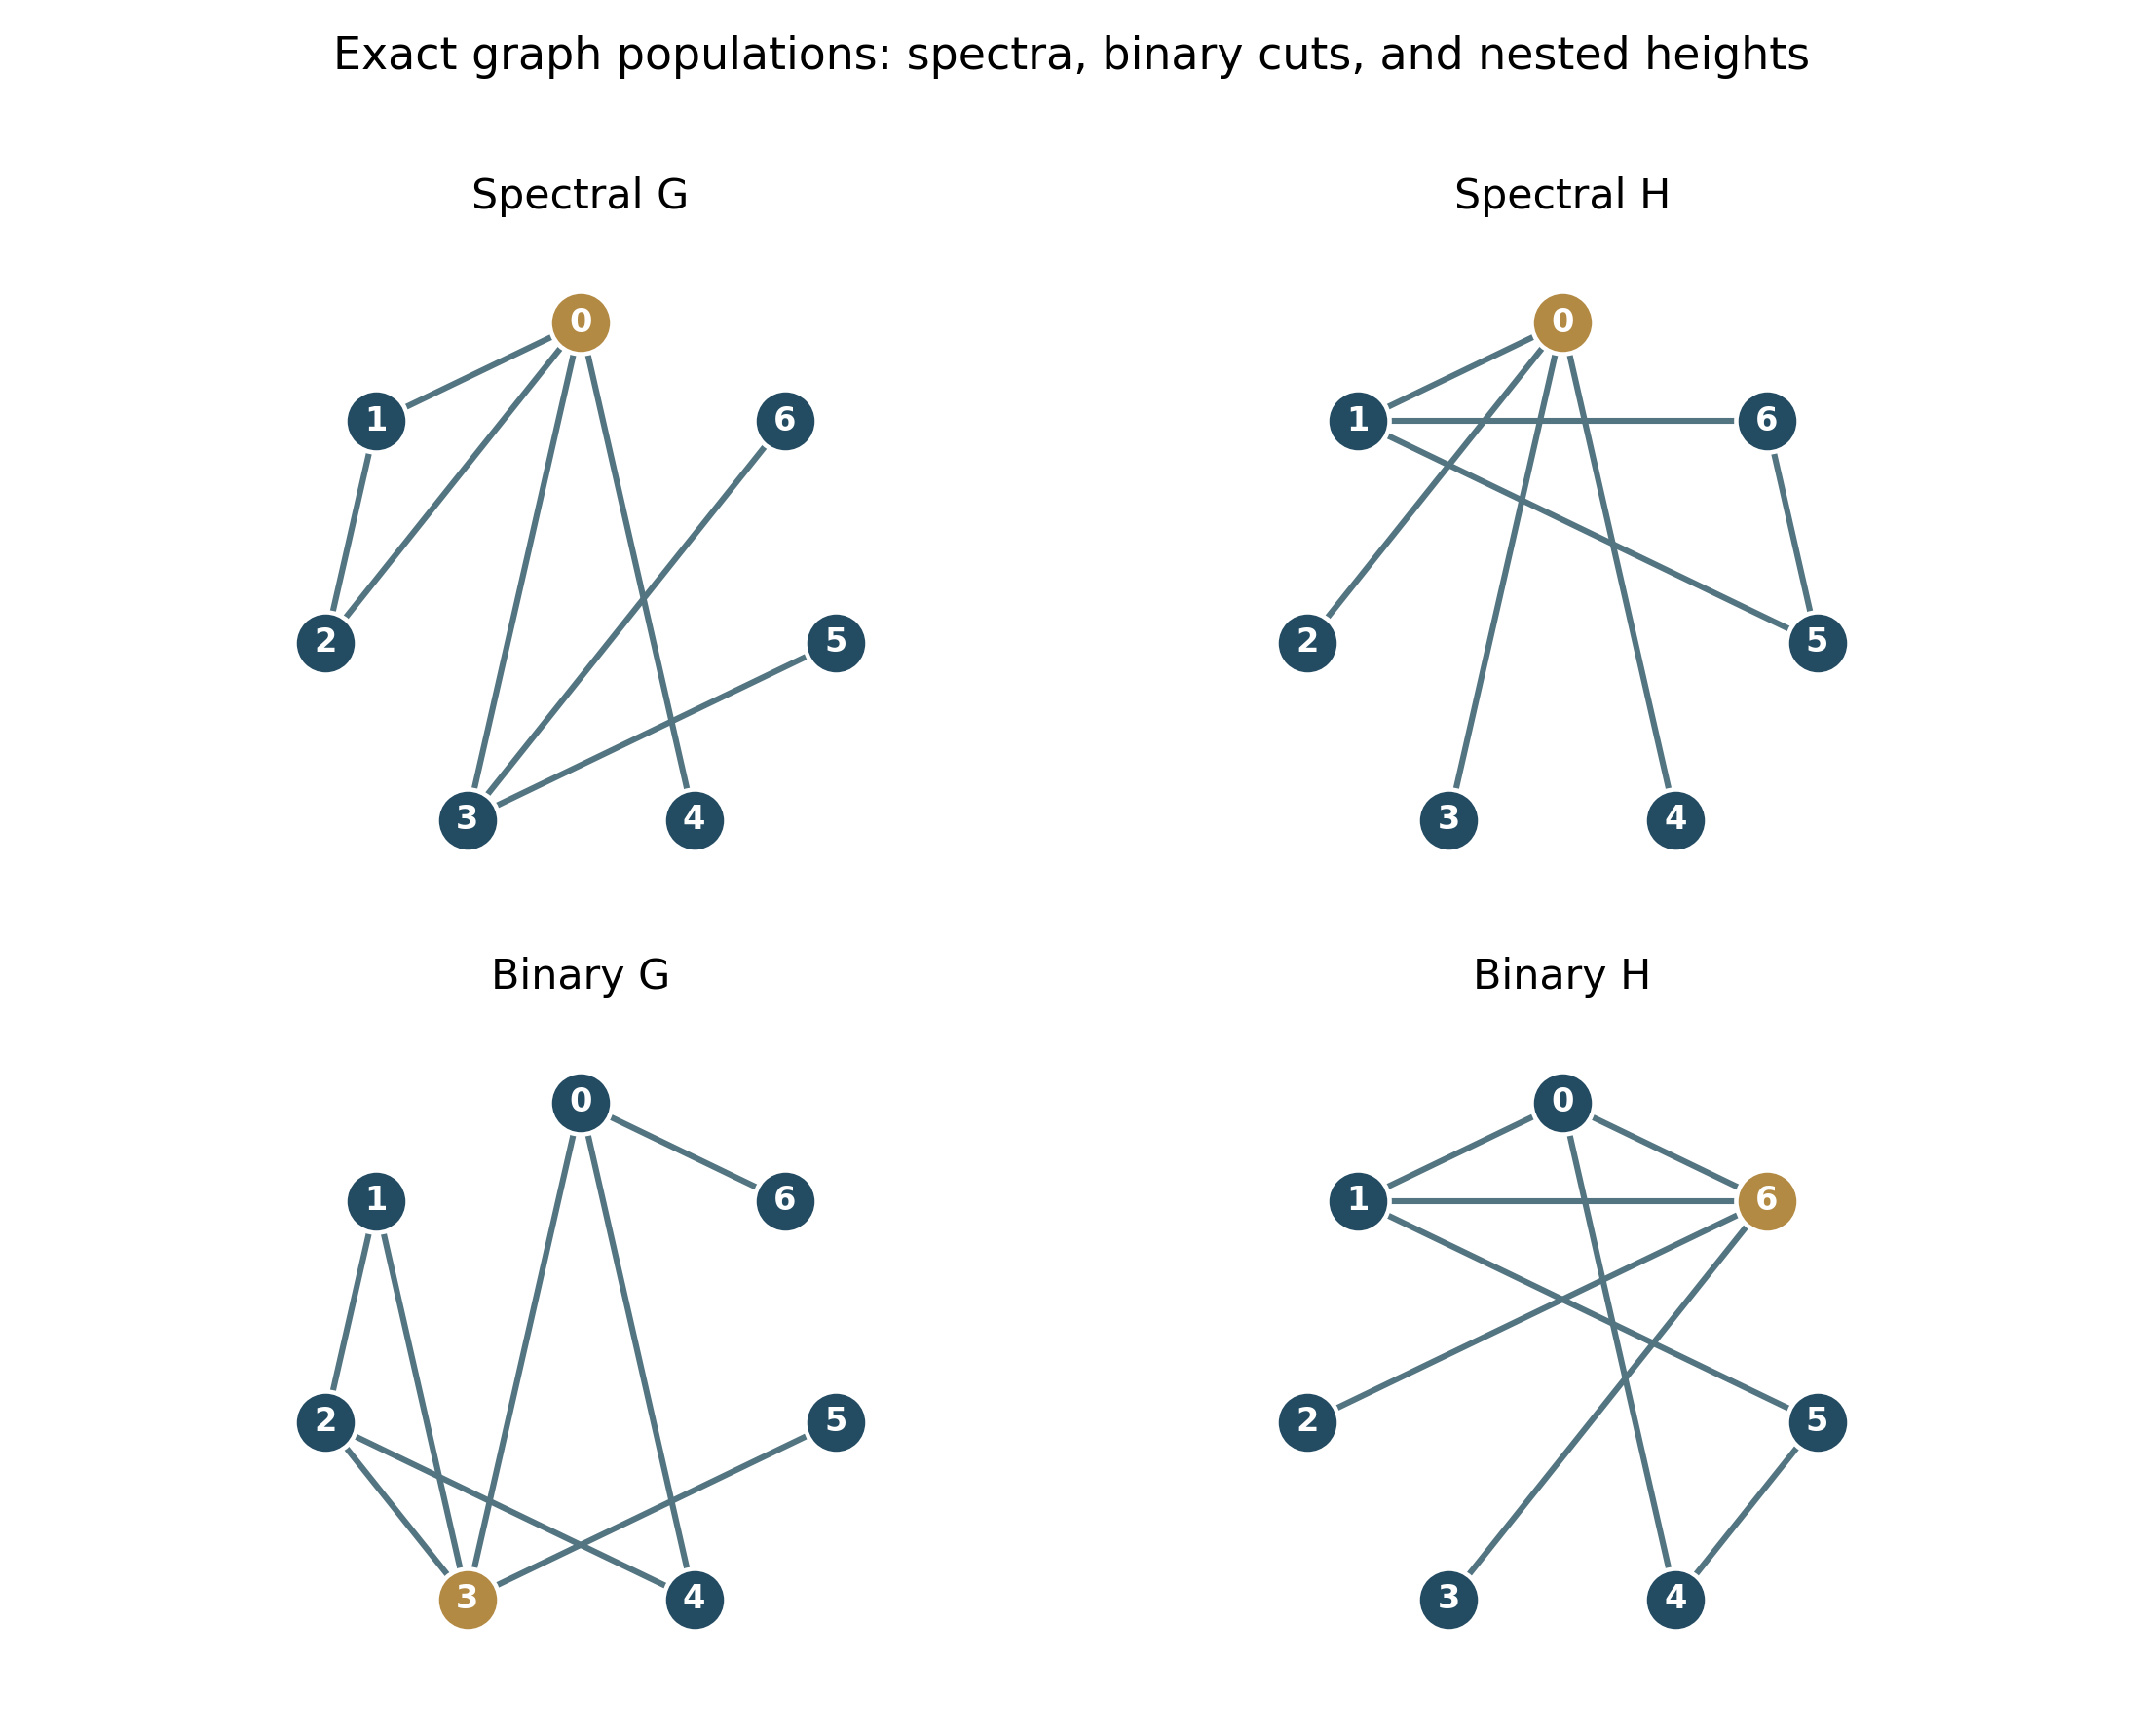
\includegraphics{assets/graph_pairs.png}
\caption{Exact reference graphs. Top: equal Laplacian spectra. Bottom:
equal complete binary cut-volume census. Vertex labels remain original.}
\end{figure}

\hypertarget{what-the-population-observes}{%
\chapter{What the population
observes}\label{what-the-population-observes}}

\hypertarget{a-relation-before-a-prediction}{%
\section{A relation before a
prediction}\label{a-relation-before-a-prediction}}

This book begins with a finite graph and a deliberately restricted
experiment. Each vertex receives a nonnegative integer height. An edge
pays the square of the difference between its endpoint heights. We count
all height assignments having a specified total height and a specified
energy. We then ask how much of the original relation between vertices
survives in those counts. The question concerns the information
contained in an exact mathematical observation. It does not require
interpreting vertices as people, particles, assets, or physical
locations.

The restriction is essential. If an experiment reports every vertex
height and every labeled edge contribution, the graph can be read
directly from the report. The interesting problem begins after that
correspondence is removed. A histogram may tell us how many assignments
have a certain energy without telling us which assignments they were.
The resulting observation can preserve information that a familiar
spectrum loses, while still losing information of its own. Establishing
either possibility requires a proof or a concrete exact comparison.

There are consequently two distinct tasks. The forward task computes the
population produced by a supplied graph. The inverse task decides what a
population determines about its source. An efficient and correct forward
computation does not settle the inverse question. Nor does a pair of
distinguishable examples establish that every pair is distinguishable.
Throughout the manuscript, reconstruction is a question to investigate,
not an advertised theorem.

\hypertarget{objects-assignments-and-the-meaning-of-a-coefficient}{%
\section{Objects, assignments, and the meaning of a
coefficient}\label{objects-assignments-and-the-meaning-of-a-coefficient}}

Let \(G=(V,E)\) be a finite simple undirected graph with labeled vertex
set \[
V=\{0,1,\ldots,k-1\},\qquad k\ge1.
\] An edge is an unordered pair of distinct vertices, and each unordered
pair occurs at most once. Write \(d_i\) for the degree of vertex \(i\),
and \(A_{ij}\in\{0,1\}\) for the adjacency matrix. Connectedness will be
required explicitly when needed. The basic formal counting series itself
is defined for disconnected graphs as well.

A height profile is a vector
\(a=(a_0,\ldots,a_{k-1})\in\mathbb Z_{\ge0}^k\). Its volume, energy, and
span are \[
|a|=\sum_i a_i,\qquad
E_G(a)=\sum_{\{i,j\}\in E}(a_i-a_j)^2,\qquad
h(a)=\max_i a_i-\min_i a_i.
\] The word \textbf{volume} always means total integer height. It is not
a Euclidean volume, a determinant, the number of occupied vertices, or
the number of nonzero levels. A profile of volume four might put height
four at one vertex, height two at two vertices, or height one at four
vertices. These assignments generally have different energies.

Define the local series \[
L_G(x,q)=\sum_{a\in\mathbb Z_{\ge0}^k}x^{|a|}q^{E_G(a)}
=\sum_{m\ge0}C_{G,m}(q)x^m.
\] The coefficient \([x^m q^e]L_G\) is the number of original labeled
assignments of volume \(m\) and energy \(e\). It does not count graph
automorphism orbits. If a symmetry exchanges two assignments, both
remain in the population. This convention makes coefficients directly
comparable to enumeration and avoids inserting unannounced symmetry
factors.

\textbf{Theorem SNG-F01 (finite local coefficients).} For every finite
graph on \(k\ge1\) vertices and every \(m\ge0\), \(C_{G,m}(q)\) is a
polynomial in \(q\) with nonnegative integer coefficients. Its
coefficient sum is \[
C_{G,m}(1)=\binom{m+k-1}{k-1}.
\] If \(\Delta=\max_i d_i\), its degree is at most \(\Delta m^2\).

\emph{Proof.} The nonnegative integer solutions of
\(a_0+\cdots+a_{k-1}=m\) are the weak compositions of \(m\) into \(k\)
parts. The usual separator construction gives their number as the
displayed binomial coefficient. In particular, there are finitely many
terms in \(C_{G,m}\). Every energy is a nonnegative integer. Moreover,
\[
E_G(a)=\sum_i d_i a_i^2-2\sum_{\{i,j\}\in E}a_i a_j
\le\Delta\sum_i a_i^2\le\Delta\Bigl(\sum_i a_i\Bigr)^2.
\] The first inequality uses nonnegativity of all heights; the second
follows by expanding the square. This proves all assertions. \(\square\)

Thus \(L_G\) is well defined as an element of \(\mathbb Z[q][[x]]\).
This assertion is formal: no choice of numerical \(x\) or \(q\), and no
convergence argument, is required. Later analytic interpretations must
separately state the region in which a formal identity can be evaluated.

\hypertarget{removing-a-repetition-that-carries-no-relational-information}{%
\section{Removing a repetition that carries no relational
information}\label{removing-a-repetition-that-carries-no-relational-information}}

Adding the same integer to every height leaves every edge difference
unchanged: \[
E_G(a+t\mathbf1)=E_G(a),\qquad |a+t\mathbf1|=|a|+kt.
\] Every nonnegative profile has a unique decomposition \[
a=b+t\mathbf1,\qquad t=\min_i a_i,\qquad \min_i b_i=0.
\] We therefore retain the normalized series \[
B_G(x,q)=\sum_{\substack{b\ge0\\\min b=0}}x^{|b|}q^{E_G(b)}.
\] The normalization removes the common-height tower, not an
assignment-specific ambiguity. It retains one explicitly specified
representative of each integer profile modulo common translation.

To distinguish assignments with one nonzero level from assignments with
several levels, introduce the full marked series \[
\mathcal B_G(x,q,z)
=\sum_{\substack{b\ge0\\\min b=0}}
x^{|b|}q^{E_G(b)}z^{\max b}.
\] The symbol \(B_G(x,q,z)\) may be used for this same three-variable
object when its arguments are displayed. In these foundational chapters,
\(\mathcal B_G\) makes the extra mark visually explicit, while
\(B_G(x,q)=\mathcal B_G(x,q,1)\). On normalized profiles, maximum height
equals span. Consequently \(z\) records a property that common
translation does not change.

\textbf{Theorem SNG-F02 (normalization and span marking).} For every
finite graph on \(k\ge1\) vertices, \[
B_G(x,q)=(1-x^k)L_G(x,q).
\] More generally, if \[
\widetilde L_G(x,q,z)=\sum_{a\ge0}x^{|a|}q^{E_G(a)}z^{h(a)},
\] then \[
\mathcal B_G(x,q,z)=(1-x^k)\widetilde L_G(x,q,z).
\] Both normalized series have nonnegative integer coefficients despite
the subtraction in these formulas.

\emph{Proof.} Use the unique decomposition \(a=b+t\mathbf1\). Energy and
span are unchanged, whereas volume increases by \(kt\). Hence
\(\widetilde L_G=\mathcal B_G\sum_{t\ge0}x^{kt}=\mathcal B_G/(1-x^k)\).
Specializing \(z=1\) gives the first identity. Each coefficient of
\(\mathcal B_G\) counts an explicitly defined finite set, proving
nonnegativity without relying on cancellation. \(\square\)

Keeping \(k\) fixed, \(B_G\) and \(L_G\) contain exactly the same formal
information: either is recovered from the other by multiplication or
division by \(1-x^k\). The span mark is a different matter. Specializing
\(z=1\) merges populations of different spans. We do not assume that
this merging can be inverted.

\begin{longtable}[]{@{}
  >{\raggedright\arraybackslash}p{(\columnwidth - 4\tabcolsep) * \real{0.3333}}
  >{\raggedright\arraybackslash}p{(\columnwidth - 4\tabcolsep) * \real{0.3333}}
  >{\raggedright\arraybackslash}p{(\columnwidth - 4\tabcolsep) * \real{0.3333}}@{}}
\toprule\noalign{}
\begin{minipage}[b]{\linewidth}\raggedright
Observation
\end{minipage} & \begin{minipage}[b]{\linewidth}\raggedright
Coefficient meaning
\end{minipage} & \begin{minipage}[b]{\linewidth}\raggedright
Correspondence deliberately removed
\end{minipage} \\
\midrule\noalign{}
\endhead
\bottomrule\noalign{}
\endlastfoot
\(L_G(x,q)\) & All profiles by total height and energy & Identity of
each profile \\
\(B_G(x,q)\) & Translation-normalized profiles by total height and
energy & Identity of each normalized profile \\
\(\mathcal B_G(x,q,z)\) & Normalized profiles by total height, energy,
and span & Identity of each profile within a marked cell \\
\([z]\mathcal B_G\) & Binary profiles, excluding the two constant
profiles & Identity of the vertex subset \\
\(B_G(1,q)\), when defined & Translation classes by energy alone & Total
height and span \\
\end{longtable}

\hypertarget{labeled-populations-can-define-unlabeled-observations}{%
\section{Labeled populations can define unlabeled
observations}\label{labeled-populations-can-define-unlabeled-observations}}

Labels specify the population being counted, but the aggregate series
does not privilege a particular labeling. Let \(\sigma:V(G)\to V(H)\) be
a graph isomorphism. Transport a profile by \(a'_{\sigma(i)}=a_i\). This
operation permutes the coordinates; it does not merge assignments.

\textbf{Theorem SNG-F03 (isomorphism invariance with original
multiplicity).} Graph isomorphisms preserve \(L_G\), \(B_G\), and
\(\mathcal B_G\).

\emph{Proof.} Coordinate permutation is a bijection on profiles and on
normalized profiles. It preserves the sum, minimum, and maximum of their
coordinates. Since it is a bijection on edges, it preserves the sum of
squared differences. Each coefficient population is therefore carried
bijectively to the corresponding population for \(H\). \(\square\)

The theorem proves one implication: isomorphic graphs have equal
observations. It does not prove the converse. An invariant is allowed to
identify nonisomorphic graphs. The inverse program investigates whether
this particular invariant does so, and, if it does, which features
remain recoverable despite that blindness.

For example, a single edge has energy \((a_0-a_1)^2\). A normalized
nonzero profile is either \((h,0)\) or \((0,h)\), so \[
\mathcal B_{K_2}(x,q,z)=1+2\sum_{h\ge1}x^h q^{h^2}z^h.
\] The coefficient two records the two original assignments. It is not
replaced by one because the edge has an endpoint-exchanging symmetry.
This elementary example is a useful check on every later convention.

For a slightly richer example, take the three-vertex path \(0-1-2\). Its
degrees are \((1,2,1)\), and direct enumeration gives \[
[x]B_G=2q+q^2,
\qquad
[x^2]B_G=2q+q^2+2q^4+q^8.
\] At volume two, placing both units at an endpoint contributes \(q^4\),
placing both at the middle contributes \(q^8\), and placing one unit at
each of two vertices contributes the remaining terms. The full mark
separates the two mechanisms: \[
[x^2]\mathcal B_G
=z(2q+q^2)+z^2(2q^4+q^8).
\] The span-one term consists of three binary subsets. The span-two term
consists of three profiles concentrated at one vertex. Setting \(z=1\)
adds these two populations without recording which mechanism produced
each contribution.

At volume three, the unnormalized count contains the all-one profile,
whose energy is zero. The normalized coefficient removes that one
translation of the zero profile: \[
[x^3]B_G=2q^2+4q^5+2q^9+q^{18}.
\] Its coefficient sum is nine, compared with ten weak compositions of
three into three parts. Thus normalization changes an original
population by a precisely specified quotient rule; it does not
arbitrarily discard an inconvenient solution. A useful calculation
record should make this distinction visible whenever normalized and
unnormalized outputs appear together.

For comparison, the triangle has \[
[x]B_{K_3}=3q^2,
\qquad [x^2]B_{K_3}=3q^2+3q^8.
\] Already the first coefficient distinguishes the two graphs because
their degree histograms differ. Such an example checks conventions but
is not a demanding test of an inverse method. Later comparisons should
deliberately match the simpler observations before attributing a
discrepancy to a deeper mechanism.

\hypertarget{what-a-result-in-this-book-means}{%
\section{What a result in this book
means}\label{what-a-result-in-this-book-means}}

Several mathematical activities appear together, and their conclusions
should not be conflated. A proved identity between formal series applies
coefficientwise to every allowed input. An exact finite computation
establishes the cells actually enumerated. A comparison through volume
\(M\) establishes equality or discrepancy through that volume. A
numerical graph search may suggest a pattern without proving that no
later counterexample exists. An analytic theorem requires its own
convergence and continuation hypotheses even when its starting Euler
factors have exact coefficients.

The book therefore separates mathematical propositions, software
behavior, finite examples, and research targets. The numbered
foundational statements below are proved from their displayed
hypotheses. They are mathematical statements, not assertions that a
proof assistant checked the implementation. Software validation supplies
another kind of evidence: it tests whether a program realizes the stated
mathematics on the cases examined.

\begin{longtable}[]{@{}
  >{\raggedright\arraybackslash}p{(\columnwidth - 4\tabcolsep) * \real{0.3333}}
  >{\raggedright\arraybackslash}p{(\columnwidth - 4\tabcolsep) * \real{0.3333}}
  >{\raggedright\arraybackslash}p{(\columnwidth - 4\tabcolsep) * \real{0.3333}}@{}}
\toprule\noalign{}
\begin{minipage}[b]{\linewidth}\raggedright
Type of statement
\end{minipage} & \begin{minipage}[b]{\linewidth}\raggedright
Appropriate evidence
\end{minipage} & \begin{minipage}[b]{\linewidth}\raggedright
Scope of conclusion
\end{minipage} \\
\midrule\noalign{}
\endhead
\bottomrule\noalign{}
\endlastfoot
Exact forward coefficient & Enumeration, recurrence, or an exact
algebraic identity & The stated coefficient or family \\
Prefix agreement & Equal coefficient dictionaries through a declared
volume & That finite prefix \\
Strict separation & One exact unequal coefficient & The two observations
differ \\
Reconstruction theorem & A proof recovering isomorphism from equality &
Every graph in the proved class \\
Reconstruction conjecture & A precise proposed implication & A question,
not an established result \\
Analytic continuation & A convergent factorization on a stated domain &
That domain and chosen branches \\
\end{longtable}

There is also a useful distinction between a new question for this
project and a historically new mathematical construction. Integer graph
lattices, Ising-type observations, graph partition functions, and
inverse problems all have substantial literatures. The graph cut-lattice
viewpoint belongs to established background, including {[}BHN1997{]}.
Binary energy populations overlap directly with graph Ising polynomials
with an external field; {[}AM2009{]} is relevant background. General
graph reconstruction from families of observations must be compared
carefully with the much richer families studied in {[}Lovasz2012{]}. No
historical priority claim is needed to make the present calculations
worthwhile.

The particular program here is to track exactly which relational
information survives a succession of increasingly marked arithmetic
height observations. Its central difficulty is \textbf{lost
correspondence}. Counts can be exact while the identities responsible
for them are absent. An inverse theorem must recover what that loss
hides; an impossibility theorem must demonstrate that the lost
information cannot be recovered from the declared observation. Both are
substantive mathematical outcomes.

The next chapter puts the translation quotient on an integral lattice.
The third chapter explains why multiple nested boundaries retain more
information than a single binary cut and why repeated levels cannot be
omitted. The fourth chapter turns coefficient order into a precise
hierarchy of visibility, beginning with degrees and degree mixing and
ending with the open reconstruction question.

\hypertarget{graphs-integral-cut-lattices-and-the-height-mark}{%
\chapter{Graphs, integral cut lattices, and the height
mark}\label{graphs-integral-cut-lattices-and-the-height-mark}}

\hypertarget{the-quadratic-form-and-its-kernel}{%
\section{The quadratic form and its
kernel}\label{the-quadratic-form-and-its-kernel}}

Let \(G\) have adjacency matrix \(A\), degree matrix
\(D=\operatorname{diag}(d_i)\), and combinatorial Laplacian
\(\Delta_G=D-A\). Expanding each square in the definition of energy
gives \[
E_G(a)=a^\top\Delta_Ga
=\sum_i d_i a_i^2-2\sum_{\{i,j\}\in E}a_i a_j.
\] The Laplacian is symmetric and positive semidefinite. This is
stronger than a numerical spectral observation: the displayed edge-sum
expression proves positivity for every real vector.

\textbf{Theorem SNG-F04 (zero energy and component constants).} For
\(a\in\mathbb R^k\), \(E_G(a)=0\) if and only if \(a\) is constant on
each connected component. In particular, for connected \(G\),
\(\ker\Delta_G=\mathbb R\mathbf1\).

\emph{Proof.} A finite sum of nonnegative squares vanishes precisely
when every summand vanishes. Thus adjacent vertices must have equal
coordinates. Equality propagates along paths, proving constancy on every
component. The converse follows because every edge lies within a
component. Finally, \(\Delta_Ga=0\) implies \(a^\top\Delta_Ga=0\);
component constancy also directly implies \(\Delta_Ga=0\). \(\square\)

For connected graphs, the zero direction is common translation. For
disconnected graphs there are additional zero directions: different
components can be shifted independently. This difference matters when a
formal series is evaluated without its height mark. Quotienting only by
global translation does not remove all zero modes of a disconnected
graph.

\hypertarget{an-orientation-is-a-bookkeeping-choice}{%
\section{An orientation is a bookkeeping
choice}\label{an-orientation-is-a-bookkeeping-choice}}

Choose an arbitrary orientation of every edge. Let \(\partial\) be the
\(|E|\)-by-\(k\) matrix whose row for an oriented edge \(i\to j\) has
\(-1\) in column \(i\), \(+1\) in column \(j\), and zero elsewhere. Then
\[
(\partial a)_{i\to j}=a_j-a_i,
\qquad \partial^\top\partial=\Delta_G.
\] The image \[
\mathcal C(G)=\partial\mathbb Z^k\subseteq\mathbb Z^E
\] is the integral cut, or tension, lattice in this convention. It
consists of edge differences produced by integer vertex potentials. An
arbitrary integer edge vector need not lie in this image: differences
around every oriented cycle must sum to zero.

Reversing an edge orientation multiplies the corresponding coordinate by
\(-1\). This is an integral orthogonal transformation of
\(\mathbb Z^E\). It preserves inner products, squared lengths, and every
energy count. An orientation is therefore needed to write vectors, but
none of the observations depends on it.

\textbf{Theorem SNG-F05 (integer quotient and cut-lattice coordinates).}
If \(G\) is connected, \(a\mapsto\partial a\) induces an isomorphism of
abelian groups \[
\mathbb Z^k/\mathbb Z\mathbf1\ \cong\ \mathcal C(G).
\] Under this isomorphism, squared lattice length is \(E_G(a)\). If a
root vertex \(r\) is fixed and \(\Delta_G^{(r)}\) is obtained by
deleting row and column \(r\), the energy in rooted coordinates is the
positive-definite integral form \[
u^\top\Delta_G^{(r)}u,\qquad u\in\mathbb Z^{k-1}.
\]

\emph{Proof.} The map is surjective onto its stated image. Its integer
kernel consists of constant integer vectors by Theorem SNG-F04. The
first isomorphism theorem gives the quotient description. The equality
of squared length and energy follows from
\(\partial^\top\partial=\Delta_G\). Every integer translation class has
a unique representative with coordinate \(a_r=0\), obtained by
subtracting \(a_r\mathbf1\). Substitution gives the reduced quadratic
form. If that form vanishes, its full representative is constant and has
root coordinate zero, so it is zero. The form is therefore positive
definite. \(\square\)

The root-zero representative is particularly convenient for linear
algebra. It may have negative coordinates. The minimum-zero
representative used by \(B_G\) is particularly convenient for a
nonnegative height mark. These are two coordinate choices on the same
quotient, not two different populations of translation classes.

\hypertarget{a-determinant-that-counts-trees}{%
\section{A determinant that counts
trees}\label{a-determinant-that-counts-trees}}

The determinant of the reduced Laplacian gives a useful consistency
check connecting the integer form with ordinary graph structure. We
include a proof because it makes clear which combinatorial data enter
the lattice and because no floating-point eigenvalue calculation is
needed.

\textbf{Theorem SNG-F06 (matrix-tree determinant).} For connected \(G\)
on \(k\ge2\) vertices and any root \(r\), \[
\det\Delta_G^{(r)}=\tau(G),
\] where \(\tau(G)\) is the number of spanning trees of \(G\).

\emph{Proof.} Delete column \(r\) of \(\partial\), obtaining \(M\). Then
\(\Delta_G^{(r)}=M^\top M\). The Cauchy--Binet formula gives \[
\det(M^\top M)
=\sum_{F\subseteq E,\ |F|=k-1}\det(M_F)^2,
\] where \(M_F\) restricts \(M\) to the selected edge rows. If \((V,F)\)
is disconnected, choose a component not containing \(r\). Its indicator
vector, restricted to nonroot coordinates, is a nonzero vector killed by
\(M_F\), so the determinant is zero. A connected graph with \(k\)
vertices and \(k-1\) edges is a tree. For a tree, the determinant is
\(\pm1\): repeatedly choose a nonroot leaf, expand in its column, and
delete the leaf and its incident edge. Each expansion contributes a sign
and an entry \(\pm1\); the final empty determinant is one. Thus exactly
the spanning-tree subsets contribute one to the sum. \(\square\)

The theorem identifies a lattice determinant. It does not say that this
determinant determines the lattice or the graph. Many nonisomorphic
graphs have the same number of spanning trees. Even a complete list of
real Laplacian eigenvalues describes the quadratic form only up to real
orthogonal change of coordinates, whereas an integer height population
depends on where the integer lattice sits inside that real space.

This distinction is elementary but decisive. A real orthogonal matrix
preserves lengths of all real vectors. It need not map
\(\mathbb Z^{k-1}\) to itself. An integral change of lattice basis must
lie in \(\mathrm{GL}_{k-1}(\mathbb Z)\), a much more restrictive group.
Consequently equal real spectra alone do not supply a bijection between
integer height profiles.

\hypertarget{unmarked-theta-and-the-extra-information-in-a-mark}{%
\section{Unmarked theta and the extra information in a
mark}\label{unmarked-theta-and-the-extra-information-in-a-mark}}

For connected \(G\), the unmarked cut-lattice theta series is \[
\Theta_G(q)=\sum_{u\in\mathbb Z^{k-1}}
q^{u^\top\Delta_G^{(r)}u}.
\] Changing the root changes the integral coordinates but not the
translation classes being counted. Likewise, an integral isometry of cut
lattices preserves this series. Graph cut lattices and their
relationship with graph structure have a substantial established theory;
{[}BHN1997{]} provides relevant background. No converse classification
from theta-series equality is assumed here.

\textbf{Theorem SNG-F07 (finite energy shells and convergence).} If
\(G\) is connected and \(k\ge2\), every energy coefficient of
\(\Theta_G\) is finite, and the series converges absolutely for
\(|q|<1\). Moreover, \[
\Theta_G(q)=B_G(1,q)
\] as a coefficientwise formal energy series and, for \(|q|<1\), as a
convergent sum.

\emph{Proof.} In root-zero coordinates, join \(r\) to each vertex \(i\)
by a simple path of length at most \(k-1\). The telescoping sum of edge
differences and Cauchy--Schwarz give \[
u_i^2\le(k-1)E_G(u),\qquad
\sum_{i\ne r}u_i^2\le(k-1)^2E_G(u).
\] An energy shell \(E_G(u)=e\) therefore lies in a finite integer box.
If \(0<\rho<1\), then \[
\rho^{E_G(u)}
\le\rho^{\|u\|_2^2/(k-1)^2},
\] and the sum of the right side is a product of convergent
one-dimensional Gaussian sums. The case \(q=0\) is immediate. Finally,
root-zero and minimum-zero profiles each select exactly one
representative of every translation class and preserve energy. Their
energy sums coincide. \(\square\)

For a disconnected graph with at least two nonempty components,
\(B_G(1,q)\) generally diverges, even for \(0<q<1\): set one component
to height zero and another to arbitrary common height. These are
distinct normalized zero-energy profiles. The true cut lattice quotients
by componentwise constants, while our normalization quotients by one
global constant. Those constructions must not be silently identified.

The total-height mark retains a feature that the lattice norm alone does
not name. For an arbitrary integer representative \(a\), define \[
\mu([a])=\sum_i a_i-k\min_i a_i,
\qquad
\eta([a])=\max_i a_i-\min_i a_i.
\] Both are well defined on translation classes. They equal volume and
span on the minimum-zero representative. The marked theta population is
therefore a lattice together with extra functions on its elements. An
abstract norm-preserving lattice bijection need not preserve those
functions.

\hypertarget{the-height-mark-is-an-asymmetric-gauge}{%
\section{The height mark is an asymmetric
gauge}\label{the-height-mark-is-an-asymmetric-gauge}}

The function \(\mu\) is not a linear functional on the quotient. A
change in which vertex attains the minimum changes its formula. This
nonlinearity is part of what the mark observes, rather than a defect in
the normalization.

\textbf{Theorem SNG-F08 (gauge identities and complement reciprocity).}
On \(\mathbb Z^k/\mathbb Z\mathbf1\), the functions \(\mu\) and \(\eta\)
satisfy \[
\mu(\alpha+\beta)\le\mu(\alpha)+\mu(\beta),
\qquad \mu(t\alpha)=t\mu(\alpha)\quad(t\in\mathbb Z_{\ge0}),
\] \[
\mu(\alpha)+\mu(-\alpha)=k\eta(\alpha).
\] For fixed span \(h\), put \(B_{G,h}(x,q)=[z^h]\mathcal B_G(x,q,z)\).
This is a polynomial and obeys \[
B_{G,h}(x,q)=x^{kh}B_{G,h}(x^{-1},q).
\]

\emph{Proof.} For representatives \(a,b\),
\(\min_i(a_i+b_i)\ge\min_i a_i+\min_i b_i\); subtracting \(k\) times
this inequality from the coordinate sum proves subadditivity.
Nonnegative integer homogeneity is immediate. Also
\(\min(-a)=-\max(a)\), so adding the formulas for \(\mu([a])\) and
\(\mu([-a])\) gives \(k(\max a-\min a)\). For reciprocity, every
normalized span-\(h\) profile has coordinates in \(\{0,\ldots,h\}\), so
the set is finite. The involution \(a\mapsto h\mathbf1-a\) preserves
energy, exchanges minimum and maximum, and changes volume from \(m\) to
\(kh-m\). Summing over the involution proves the identity. \(\square\)

The reciprocity is spanwise. After setting \(z=1\), profiles with many
different \(h\) are merged, and there is no single factor \(x^{kh}\)
applying to their sum. This is a concrete example of a relation visible
with the full mark but not immediately expressible after that mark is
forgotten.

\begin{longtable}[]{@{}
  >{\raggedright\arraybackslash}p{(\columnwidth - 4\tabcolsep) * \real{0.3333}}
  >{\raggedright\arraybackslash}p{(\columnwidth - 4\tabcolsep) * \real{0.3333}}
  >{\raggedright\arraybackslash}p{(\columnwidth - 4\tabcolsep) * \real{0.3333}}@{}}
\toprule\noalign{}
\begin{minipage}[b]{\linewidth}\raggedright
Structure retained
\end{minipage} & \begin{minipage}[b]{\linewidth}\raggedright
Natural coordinate change
\end{minipage} & \begin{minipage}[b]{\linewidth}\raggedright
Quantity necessarily preserved
\end{minipage} \\
\midrule\noalign{}
\endhead
\bottomrule\noalign{}
\endlastfoot
Real quadratic space & Real orthogonal isometry & Real energy \\
Integral cut lattice & Integral lattice isometry & Integer energy
shells \\
Height-marked lattice population & Bijection preserving energy and
\(\mu\) & Joint volume-energy counts \\
Fully marked population & Bijection preserving energy, \(\mu\), and
\(\eta\) & Joint volume-energy-span counts \\
\end{longtable}

These rows are preservation requirements, not a claim that every
bijection in a lower row arises from graph relabeling. The inverse
problem asks precisely how much of the source graph is forced by
increasingly restrictive observations.

\hypertarget{two-endpoint-calculations}{%
\section{Two endpoint calculations}\label{two-endpoint-calculations}}

At \(q=1\), energy is forgotten completely. Every coordinate contributes
its own geometric series, so \[
L_G(x,1)=\frac1{(1-x)^k},\qquad
B_G(x,1)=\frac{1-x^k}{(1-x)^k}.
\] No edge appears in these expressions. At \(q=0\), only zero-energy
assignments remain. If the connected components have sizes
\(k_1,\ldots,k_c\), Theorem SNG-F04 gives \[
L_G(x,0)=\prod_{j=1}^c\frac1{1-x^{k_j}},
\qquad
B_G(x,0)=(1-x^k)\prod_{j=1}^c\frac1{1-x^{k_j}}.
\] For connected graphs this reduces to \(L_G(x,0)=1/(1-x^k)\) and
\(B_G(x,0)=1\). Thus both endpoints erase most graph structure: one
ignores every edge energy, and the other retains only exact agreement
within components. An inverse experiment must retain intermediate energy
information rather than relying on these endpoint values alone.

\hypertarget{disjoint-unions-and-recoverable-component-sizes}{%
\section{Disjoint unions and recoverable component
sizes}\label{disjoint-unions-and-recoverable-component-sizes}}

The unnormalized series factors naturally over independent components.
Normalization by one global minimum does not factor in the same way,
because choosing the minimum of the combined profile couples the choice
of representatives in its components. This is a useful instance in which
an exact quotient must be carried through an otherwise simple product
rule.

\textbf{Theorem SNG-F19 (component factorization and its endpoint
inverse).} For graphs \(G,H\) on \(k,\ell\ge1\) vertices, \[
L_{G\sqcup H}(x,q)=L_G(x,q)L_H(x,q),
\] \[
B_{G\sqcup H}(x,q)
=\frac{1-x^{k+\ell}}{(1-x^k)(1-x^\ell)}B_G(x,q)B_H(x,q).
\] Moreover, the zero-energy series \(L_G(x,0)\) determines the multiset
of connected-component sizes.

\emph{Proof.} A profile on a disjoint union is uniquely a pair of
profiles on its components. Both volume and energy add, proving the
first identity. Substituting \(L_G=B_G/(1-x^k)\), and the corresponding
formulas for \(H\) and the union, proves the second identity in formal
series. For the final assertion, let \(c_j\) be the number of components
of size \(j\). Then \[
L_G(x,0)=\prod_{j\ge1}(1-x^j)^{-c_j}.
\] Formal logarithms are legitimate because the constant term is one.
Expanding \(-\log(1-x^j)=\sum_{r\ge1}x^{jr}/r\), put
\(b_n=n[x^n]\log L_G(x,0)\). Then \[
b_n=\sum_{j\mid n}j c_j.
\] Recover \(c_1=b_1\) and recursively \[
c_n=\frac1n\left(b_n-\sum_{\substack{j\mid n\\j<n}}j c_j\right).
\] This uniquely determines every component-size multiplicity. Only
finitely many are nonzero. \(\square\)

The inverse statement is deliberately modest. Zero energy knows
component sizes but not the edges within a component. A path and a
complete graph on the same connected vertex set have identical
zero-energy series. The formal logarithm extracts exactly the available
component information without pretending that it contains finer internal
structure.

There is a related warning about the full span mark. The span of a
concatenated pair of arbitrary profiles depends on their relative
vertical placement, not just on the two individual spans. Consequently
one should not multiply \(\mathcal B_G\) and \(\mathcal B_H\) and
declare the result to be \(\mathcal B_{G\sqcup H}\). A correct marked
factorization would need enough additional data to retain minima,
maxima, and their relative shifts. The scalar unnormalized product
avoids that missing correspondence because it sums actual coordinates
before applying a quotient.

The cut-lattice description clarifies why integer heights are a useful
meeting point. They retain the arithmetic placement of a quadratic form,
while their minimum-zero representatives supply a nonlinear order mark.
The next chapter expresses that order mark through nested threshold
sets. This reveals precisely what lies beyond a single binary cut.

\hypertarget{nested-heights-and-the-interaction-of-boundaries}{%
\chapter{Nested heights and the interaction of
boundaries}\label{nested-heights-and-the-interaction-of-boundaries}}

\hypertarget{a-height-profile-is-a-stack-of-threshold-sets}{%
\section{A height profile is a stack of threshold
sets}\label{a-height-profile-is-a-stack-of-threshold-sets}}

A binary profile chooses a subset of vertices: height one on the subset
and zero outside. A general integer profile chooses several nested
subsets. This description is exact, but only if consecutive threshold
sets are allowed to be equal. A jump of three at one vertex crosses
three integer levels even if the set of vertices above those levels
never changes.

For a normalized profile \(a\ge0\) with \(\min a=0\) and \(\max a=h\),
define \[
S_t(a)=\{i\in V:a_i\ge t\},\qquad 1\le t\le h.
\] Then \[
\varnothing\ne S_h\subseteq S_{h-1}\subseteq\cdots\subseteq S_1\subsetneq V,
\qquad
a=\sum_{t=1}^h\mathbf1_{S_t}.
\] The inclusions are weak. Replacing them by strict inclusions changes
the population by discarding legitimate profiles.

\textbf{Theorem SNG-F09 (threshold-chain bijection).} Normalized
profiles of span \(h\ge1\) are in bijection with weakly nested chains of
\(h\) nonempty proper vertex subsets. The inverse map is
\(a_i=\#\{t:i\in S_t\}\), and \[
|a|=\sum_{t=1}^h|S_t|.
\]

\emph{Proof.} Threshold sets of a profile have the stated nesting.
Because some coordinate is zero, \(S_1\) is proper; because some
coordinate is \(h\), \(S_h\) is nonempty. Conversely, nesting implies
that, for each vertex, membership occurs at an initial segment of the
thresholds. Thus the formula for \(a_i\) gives exactly the original
membership sets when thresholds are taken again. A vertex outside
\(S_1\) has height zero and a vertex in \(S_h\) has height \(h\),
proving normalization and span. The volume identity follows by counting
all incidences \((i,t)\) with \(i\in S_t\) in two orders. \(\square\)

The chain is not an auxiliary encoding with multiple extensions. It is
uniquely determined by the original profile, and it reconstructs that
profile uniquely. Consequently a chain-based counting algorithm
preserves original assignment multiplicity without an additional
correction factor.

\hypertarget{squared-differences-do-not-add-level-by-level}{%
\section{Squared differences do not add level by
level}\label{squared-differences-do-not-add-level-by-level}}

Write \(c_G(S)=|\partial S|\) for the number of edges with one endpoint
in \(S\) and one outside. For disjoint vertex sets \(U,W\), write
\(e_G(U,W)\) for the number of edges joining them. The ordinary integer
coarea identity says \[
\sum_{\{i,j\}\in E}|a_i-a_j|=\sum_{t=1}^h c_G(S_t).
\] Our energy uses squares, so this identity alone is insufficient. An
edge crossing two levels contributes four, not two. Cross terms record
which nested boundaries are crossed by the same edge.

\textbf{Theorem SNG-F10 (nested-boundary energy formula).} For the
threshold chain of a normalized profile, \[
E_G(a)=\sum_{t=1}^h c_G(S_t)
+2\sum_{1\le r<t\le h}e_G(S_t,V\setminus S_r).
\] Equivalently, \[
E_G(a)=\sum_{r,t=1}^h
e_G\bigl(S_{\max(r,t)},V\setminus S_{\min(r,t)}\bigr).
\]

\emph{Proof.} Use the oriented edge-difference matrix \(\partial\) from
Chapter 2 and substitute \(a=\sum_t\mathbf1_{S_t}\) into
\(E_G(a)=\|\partial a\|_2^2\). Diagonal inner products equal
\(c_G(S_t)\). If \(S_t\subseteq S_r\), an edge contributes to both
gradients exactly when it joins \(S_t\) to \(V\setminus S_r\). On such
an edge the two gradient signs agree, irrespective of the chosen
orientation; otherwise at least one gradient is zero. Their inner
product is therefore \(e_G(S_t,V\setminus S_r)\). Expanding the squared
norm proves the first formula, and pairing the two orders of each
off-diagonal term proves the second. \(\square\)

An edgewise proof gives the same mechanism. If endpoint heights are
\(u<v\), the edge crosses exactly \(v-u\) thresholds. The ordered pairs
of crossed thresholds number \((v-u)^2\). The double sum counts those
pairs edge by edge. This argument also explains why repeated threshold
sets must remain: an edge can cross several numerically different
thresholds whose vertex subsets happen to coincide.

The formula concerns pairwise edge energies throughout. The cross terms
are interactions between observations of nested boundaries; they do not
turn the graph Hamiltonian into a new three-body or higher-body edge
law. Several boundaries can jointly reveal information that isolated
boundary histograms lose, even though the underlying energy remains a
sum over edges.

\hypertarget{two-examples-where-repetition-matters}{%
\section{Two examples where repetition
matters}\label{two-examples-where-repetition-matters}}

Consider the path \(0-1-2\). For \(a=(0,2,2)\), the threshold chain is
\[
S_1=S_2=\{1,2\}.
\] Each set has cut size one. The sum of the two cut sizes is two, but
the actual energy is \((0-2)^2+(2-2)^2=4\). The cross term contributes
the missing two, because one edge joins \(S_2\) to \(V\setminus S_1\). A
strict-chain enumeration would omit this profile entirely.

For \(a=(0,1,3)\), the same path gives \[
S_1=\{1,2\},\qquad S_2=S_3=\{2\}.
\] The diagonal cut sum is three. The boundaries of \(S_1\) and \(S_2\)
lie on different edges, so their overlap term is zero; the same holds
for \(S_1,S_3\). The repeated pair \(S_2,S_3\) contributes two. The
total is five, agreeing with \(1^2+2^2\).

\begin{longtable}[]{@{}
  >{\raggedright\arraybackslash}p{(\columnwidth - 10\tabcolsep) * \real{0.1304}}
  >{\raggedleft\arraybackslash}p{(\columnwidth - 10\tabcolsep) * \real{0.1739}}
  >{\raggedleft\arraybackslash}p{(\columnwidth - 10\tabcolsep) * \real{0.1739}}
  >{\raggedleft\arraybackslash}p{(\columnwidth - 10\tabcolsep) * \real{0.1739}}
  >{\raggedleft\arraybackslash}p{(\columnwidth - 10\tabcolsep) * \real{0.1739}}
  >{\raggedleft\arraybackslash}p{(\columnwidth - 10\tabcolsep) * \real{0.1739}}@{}}
\toprule\noalign{}
\begin{minipage}[b]{\linewidth}\raggedright
Path profile
\end{minipage} & \begin{minipage}[b]{\linewidth}\raggedleft
Volume
\end{minipage} & \begin{minipage}[b]{\linewidth}\raggedleft
Span
\end{minipage} & \begin{minipage}[b]{\linewidth}\raggedleft
Diagonal cut sum
\end{minipage} & \begin{minipage}[b]{\linewidth}\raggedleft
Cross-term contribution
\end{minipage} & \begin{minipage}[b]{\linewidth}\raggedleft
Energy
\end{minipage} \\
\midrule\noalign{}
\endhead
\bottomrule\noalign{}
\endlastfoot
\((0,1,1)\) & 2 & 1 & 1 & 0 & 1 \\
\((0,2,2)\) & 4 & 2 & 2 & 2 & 4 \\
\((0,1,3)\) & 4 & 3 & 3 & 2 & 5 \\
\((0,1,2)\) & 3 & 2 & 2 & 0 & 2 \\
\end{longtable}

The last row is also useful. Distinct boundaries can have no overlap,
making the squared energy equal the coarea sum. There is no universal
rule replacing the cross terms by a fixed function of the individual cut
sizes. Their value depends on how the boundaries sit together in the
same graph.

A four-cycle makes this failure especially explicit while holding both
individual sizes and individual cut counts fixed. Let the cycle be
\(0-1-2-3-0\), and let \(S=\{0,1,2\}\). Consider either \(T=\{0\}\) or
\(T'=\{1\}\) as the inner threshold set. Both chains have outer size
three, inner size one, and cut counts two and two. However, \[
e_G(T,V\setminus S)=1,
\qquad e_G(T',V\setminus S)=0.
\] The two profiles are \((2,1,1,0)\) and \((1,2,1,0)\); both have
volume four and span two. Their energies are respectively six and four.
Thus even the ordered list of threshold sizes and cut counts does not
determine the height energy. One must also retain which boundary edges
are shared.

This example does not prove that two graphs with equal complete binary
cut polynomials must have different height series. Both profiles occur
in the same graph, and a global inverse implication could in principle
use information unavailable in this two-boundary summary. What the
example proves is the narrower and useful fact that the displayed chain
energy cannot be computed from its separate boundary marginals alone.

\hypertarget{an-exact-chain-expansion-of-the-marked-series}{%
\section{An exact chain expansion of the marked
series}\label{an-exact-chain-expansion-of-the-marked-series}}

Combining the bijection and energy formula gives \[
\mathcal B_G(x,q,z)=1+
\sum_{h\ge1}z^h
\sum_{\varnothing\ne S_h\subseteq\cdots\subseteq S_1\subsetneq V}
x^{\sum_t|S_t|}
q^{\sum_t c_G(S_t)+2\sum_{r<t}e_G(S_t,V\setminus S_r)}.
\] This is an identity of formal series. At a specified total volume
\(m\), only chains of length at most \(m\) can contribute, so the
coefficient remains a finite sum. The expression is also a useful
specification for an independent implementation: direct weak-composition
enumeration and threshold-chain enumeration must return the same marked
cells.

\textbf{Proposition SNG-F21 (volume-pruned chain enumeration).} Fix
\(M\ge0\). The following search visits every normalized profile of
volume at most \(M\) exactly once: emit the empty chain; for every
nonempty proper \(S_1\subsetneq V\) with \(|S_1|\le M\), emit \((S_1)\)
and recursively extend a chain \((S_1,\ldots,S_t)\) by every nonempty
\(S_{t+1}\subseteq S_t\), equal sets included, with
\(\sum_{r\le t+1}|S_r|\le M\). If each appended level is charged
\(c_G(S_{t+1})+2\sum_{r\le t}e_G(S_{t+1},V\setminus S_r)\), the
accumulated charge is the energy of the profile, the accumulated size is
its volume and the chain length is its span.

\emph{Proof.} Every emitted sequence is a weakly nested chain of
nonempty sets with proper first set, so SNG-F09 maps it to a normalized
profile of span equal to its length and volume equal to its total size.
Conversely the threshold chain of a normalized profile of volume at most
\(M\) satisfies these constraints, and each of its prefixes has total
size at most \(M\), because sizes are positive; the search therefore
reaches it through its prefixes. Distinct emitted chains differ in some
level and hence give distinct profiles, since SNG-F09 is a bijection;
and the search emits each chain once, because the chain determines the
sequence of choices that produced it. Termination follows because each
level has size at least one, so the length is at most \(M\). The charge
identity is SNG-F10 grouped by the later index \(t\) of each pair
\(r<t\): appending \(S_{t+1}\) adds its own cut and twice its overlap
with every earlier level, and with no other pair. \(\square\)

Repetitions are essential. Forbidding \(S_{t+1}=S_t\) removes exactly
the profiles in which some height between \(0\) and the span is unused,
for instance \((0,2,2)\) and \((0,1,3)\) on the path. The search is
implemented in \texttt{src/singularity/chains.py}. It shares neither its
generator nor its energy evaluation with the weak-composition engine, so
agreement of the two on complete marked histograms is a genuine
cross-check. For every labeled simple graph on at most five vertices and
every volume at most six, the two engines agree on all 142,416 marked
cells and 479,963 profiles (\texttt{results/chain\_agreement.json}).
This is a finite computation on that declared population, not a proof
beyond it.

The expansion shows exactly what a binary observation omits. The binary
sector reports one subset at a time, through its size and cut. A chain
term refers to several nested subsets in the same graph and additionally
uses their boundary-overlap counts. Separate histograms of subset sizes
and cuts do not retain the correspondence needed to form these overlaps.

This statement is directional. The full marked series certainly contains
the binary histogram because its span-one coefficient extracts it. It
does not follow that the two-variable specialization
\(B_G(x,q)=\mathcal B_G(x,q,1)\) permits that same extraction. After
span is forgotten, a cell of given volume and energy can receive both
binary and nonbinary contributions. No inversion of that mixture is
proved here.

\hypertarget{the-binary-sector-and-its-reciprocity}{%
\section{The binary sector and its
reciprocity}\label{the-binary-sector-and-its-reciprocity}}

Define the binary cut polynomial \[
I_G(x,q)=\sum_{S\subseteq V}x^{|S|}q^{c_G(S)}.
\] Its height interpretation overlaps the external-field Ising
polynomial studied in {[}AM2009{]}, subject to the stated normalization
of the energy and spin variables. The present definition is explicit, so
no external convention is needed to compute it.

\textbf{Theorem SNG-F11 (binary sector extraction).} For \(k\ge2\), \[
[z]\mathcal B_G(x,q,z)=I_G(x,q)-1-x^k.
\] Also \(I_G(x,q)=x^kI_G(x^{-1},q)\).

\emph{Proof.} A minimum-zero span-one profile takes values zero and one
and contains both values. It is uniquely the indicator of a nonempty
proper subset. Its volume is subset size and its energy is cut size. The
omitted empty and full subsets give \(1\) and \(x^k\). Complementation
preserves cut size and sends subset size to \(k-|S|\), proving
reciprocity. \(\square\)

The symmetry pairs the two sides of a cut. We count both sides as
different profiles. A side of size \(r\) and its complement of size
\(k-r\) appear at their respective powers of \(x\); when the sizes are
equal they still contribute two unless other multiplicities happen to
coincide.

\hypertarget{minimum-cuts-are-the-first-positive-energy-shell}{%
\section{Minimum cuts are the first positive energy
shell}\label{minimum-cuts-are-the-first-positive-energy-shell}}

For a connected graph on \(k\ge2\) vertices, define edge connectivity by
\[
\lambda(G)=\min_{\varnothing\ne S\subsetneq V}c_G(S)>0.
\] This definition suffices here; no equivalence with a disjoint-path
formulation is needed.

\textbf{Theorem SNG-F12 (minimum-energy shell).} Every nonzero
normalized profile of span \(h\) obeys \[
E_G(a)\ge\lambda(G)h.
\] The smallest positive energy is \(\lambda(G)\), and its full marked
population is \[
[q^{\lambda(G)}]\mathcal B_G(x,q,z)
=z\sum_{\substack{\varnothing\ne S\subsetneq V\\c_G(S)=\lambda(G)}}x^{|S|}.
\]

\emph{Proof.} For every nonnegative integer \(d\), \(d^2\ge d\). Hence
the energy is at least the absolute-difference sum, which by coarea is
\(\sum_t c_G(S_t)\). Every threshold set is nonempty and proper, so each
cut is at least \(\lambda(G)\). This gives the bound. An indicator of a
minimum cut has energy \(\lambda(G)\), so the bound is attained. If a
nonzero profile has that energy, the bound forces \(h=1\), and then its
subset must be a minimum cut. \(\square\)

For a path, \(\lambda=1\), so the first positive shell consists of the
two orientations of every bridge cut. For a triangle, \(\lambda=2\), and
its six nonempty proper subsets give \[
[q^2]\mathcal B_{K_3}(x,q,z)=3z(x+x^2).
\] These formulas identify the very first nonconstant energy sector.
They do not recover arbitrary boundary overlaps at higher energy.

\hypertarget{support-restrictions-useful-for-exact-computation}{%
\section{Support restrictions useful for exact
computation}\label{support-restrictions-useful-for-exact-computation}}

Several finite bounds follow directly from the profile interpretation.
They identify impossible marked cells before any enumeration and provide
consistency checks afterward.

\textbf{Theorem SNG-F13 (volume, span, and extreme energy).} Let
\(k\ge2\), and let \(a\) be a nonzero normalized profile of volume \(m\)
and span \(h\). Then \[
h\le m\le(k-1)h.
\] If \(G\) is connected, \[
E_G(a)\ge\max\left\{\lambda(G)h,
\left\lceil\frac{h^2}{\operatorname{diam}(G)}\right\rceil\right\}.
\] For any graph with maximum degree \(\Delta>0\), the largest energy
among normalized volume-\(m\) profiles is \(\Delta m^2\), attained
exactly by \(a=m e_i\) at maximum-degree vertices.

\emph{Proof.} Some coordinate equals \(h\), so the sum is at least
\(h\). At least one coordinate is zero and every other coordinate is at
most \(h\), giving the upper bound. The minimum-cut bound was proved
above. Choose a shortest path between a minimum-height and a
maximum-height vertex. If its length is \(\ell\), telescoping and
Cauchy--Schwarz give
\(h^2\le\ell\sum_{e\text{ on path}}(\partial a)_e^2\le\operatorname{diam}(G)E_G(a)\).
Energy is integral, giving the ceiling. Finally, the bound
\(E_G(a)\le\Delta\sum_i a_i^2\le\Delta m^2\) was proved in Chapter 1.
The profile \(m e_i\) at a maximum-degree vertex attains it. If equality
holds and \(\Delta>0\), then \(\sum_i a_i^2=m^2\). Expanding \(m^2\)
shows that all products \(a_i a_j\), \(i\ne j\), vanish; exactly one
coordinate is nonzero. Its degree must be \(\Delta\). \(\square\)

Thus only \[
\left\lceil\frac{m}{k-1}\right\rceil\le h\le m
\] can occur in a nonzero volume-\(m\) normalized population. For fixed
\(h\), complementation from Chapter 2 pairs volumes \(m\) and \(kh-m\).
A computation violating either restriction has lost a normalization
condition or a multiplicity.

Nested thresholds provide the human explanation for the hierarchy
studied next. One occupied unit reveals a degree. Two units reveal
degree mixing. Several units can occupy different heights and thereby
test several linked boundaries. The information comes from their shared
placement in one relation, not from replacing the original edge law with
an unrelated interaction.

\hypertarget{primitive-height-scale-and-exact-dilation}{%
\section{Primitive height scale and exact
dilation}\label{primitive-height-scale-and-exact-dilation}}

Repeated sets also encode a common integer scale. If every nonzero
coordinate of a normalized profile is divisible by \(d\), division by
\(d\) gives another normalized profile. Volumes and spans divide by
\(d\), while energy divides by \(d^2\). This is an exact quadratic
scaling law, not an approximation valid only at large height.

Call a nonzero normalized profile primitive when the greatest common
divisor of its coordinates is one; zeros do not change that greatest
common divisor. Let \[
\mathcal P_G(x,q,z)
=\sum_{\substack{a\ge0,\ \min a=0\\a\ne0,\ \gcd(a_0,\ldots,a_{k-1})=1}}
x^{|a|}q^{E_G(a)}z^{\max a}.
\] The zero profile is excluded because its common divisor is not a
positive scale.

\textbf{Theorem SNG-F20 (primitive-height decomposition).} For every
graph on \(k\ge2\) vertices, \[
\mathcal B_G(x,q,z)-1
=\sum_{d\ge1}\mathcal P_G(x^d,q^{d^2},z^d).
\] If \(\mu\) is the arithmetic Möbius function, characterized by
\(\sum_{d\mid n}\mu(d)=1\) for \(n=1\) and zero otherwise, then \[
\mathcal P_G(x,q,z)
=\sum_{d\ge1}\mu(d)
\bigl(\mathcal B_G(x^d,q^{d^2},z^d)-1\bigr).
\] Both identities are coefficientwise finite in every positive volume.

\emph{Proof.} Every nonzero integer profile has a unique positive
greatest common divisor \(d\), and a unique primitive quotient
\(b=a/d\). Normalization is preserved. Direct substitution gives
\(|a|=d|b|\), \(E_G(a)=d^2E_G(b)\), and \(\max a=d\max b\), proving the
first identity. For inversion, write \(T_dF=F(x^d,q^{d^2},z^d)\); then
\(T_dT_e=T_{de}\). Substitute the first identity in the proposed
inverse. The coefficient multiplying \(T_n\mathcal P_G\) is
\(\sum_{d\mid n}\mu(d)\), leaving only \(n=1\). At volume \(m>0\), only
\(d\mid m\) can contribute, so the rearrangement is finite
coefficientwise. \(\square\)

For the path example \((0,2,2)\), the primitive quotient is \((0,1,1)\):
volume two becomes four, energy one becomes four, and span one becomes
two. This decomposition distinguishes a genuinely new shape of height
profile from an integral dilation of an earlier shape. It provides
another exact observation hierarchy that can be implemented
independently of threshold-chain enumeration.

Primitive height here refers only to common divisibility of integer
coordinates. It does not mean a primitive graph, a primitive conductor
phase, or an element primitive in a different lattice. Those notions may
interact in later calculations, but their definitions must not be merged
because they share a word. The decomposition itself uses no
connectedness assumption, so it also applies when nonconstant
componentwise profiles have zero energy.

\hypertarget{visibility-depth-and-the-loss-of-correspondence}{%
\chapter{Visibility depth and the loss of
correspondence}\label{visibility-depth-and-the-loss-of-correspondence}}

\hypertarget{increasing-volume-as-an-observation-hierarchy}{%
\section{Increasing volume as an observation
hierarchy}\label{increasing-volume-as-an-observation-hierarchy}}

The coefficient \(C_{G,m}(q)=[x^m]L_G(x,q)\) reports every energy
attainable with exactly \(m\) units of nonnegative integer height,
together with original assignment multiplicities. Increasing \(m\)
enlarges the set of placements that can be tested. It does not simply
increase numerical precision in an unchanged observation. New occupancy
patterns become available: repeated occupation of one vertex, occupation
of several vertices, and different heights on linked supports.

For equal-order graphs, normalization does not change the first place at
which their scalar-height observations differ. If \(k\) is fixed,
multiplication by \(1-x^k\) has constant term one. A first nonzero
coefficient cannot be removed by that multiplication because no earlier
nonzero coefficient exists to cancel it.

The hierarchy must be specified before it is interpreted. A volume
prefix of the two-variable series is one hierarchy; a span prefix of the
fully marked series is another. The binary sector is one span layer, not
one volume layer: a binary subset of size ten has volume ten and span
one. Conversely, a one-vertex profile of height ten has the same volume
and span ten. Keeping those distinctions prevents an observation about a
binary cut polynomial from being silently transferred to an unmarked
height specialization.

\hypertarget{the-first-coefficients-can-be-read-by-hand}{%
\section{The first coefficients can be read by
hand}\label{the-first-coefficients-can-be-read-by-hand}}

Write \(e_i\) for the unit profile at vertex \(i\). At volume one the
only profiles are \(e_i\), and \[
E_G(e_i)=d_i.
\] At volume two the profiles are \(2e_i\) and \(e_i+e_j\), \(i<j\). The
latter subtracts two from the sum of endpoint degrees precisely when the
endpoints are adjacent. This is the first layer that couples local
degrees to a relation between vertices.

\textbf{Theorem SNG-F14 (coefficients through volume three).} For every
simple graph, \[
C_{G,0}(q)=1,
\qquad C_{G,1}(q)=\sum_iq^{d_i},
\] \[
C_{G,2}(q)=\sum_iq^{4d_i}
+\sum_{i<j}q^{d_i+d_j-2A_{ij}},
\] and \[
\begin{aligned}
C_{G,3}(q)={}&\sum_iq^{9d_i}
+\sum_{i\ne j}q^{4d_i+d_j-4A_{ij}}\\
&+\sum_{i<j<\ell}q^{d_i+d_j+d_\ell-2e_G(\{i,j,\ell\})}.
\end{aligned}
\] Here \(e_G(S)\) denotes the number of edges induced by \(S\). Empty
index sums are zero. For normalized coefficients, \[
[x^m]B_G=C_{G,m}-C_{G,m-k},
\] where \(C_{G,t}=0\) for \(t<0\).

\emph{Proof.} Partition the weak compositions of one, two, and three by
their positive parts. The possibilities are respectively \(1\); \(2\) or
\(1+1\); and \(3\), \(2+1\), or \(1+1+1\). Substitute each profile in \[
E_G(a)=\sum_i d_i a_i^2-2\sum_{\{i,j\}\in E}a_i a_j.
\] The pattern \(2e_i+e_j\) is indexed by ordered distinct vertices
because the heights distinguish the two positions. The three-unit
pattern is indexed by unordered triples. These are disjoint exhaustive
cases, giving the formulas without missing multiplicities. The
normalized identity is coefficient extraction from Theorem SNG-F02.
\(\square\)

The classification can be read as a table. Write \(N_d\) for the number
of vertices of degree \(d\), \(P_{a,b}^{\epsilon}\) for the number of
\textbf{ordered} pairs \((i,j)\), \(i\ne j\), with \(d_i=a\), \(d_j=b\),
\(A_{ij}=\epsilon\), and \(T_{s,t}\) for the number of unordered triples
with degree sum \(s\) spanning \(t\) edges. These statistics are defined
from degrees and adjacency alone.

\begin{longtable}[]{@{}
  >{\raggedleft\arraybackslash}p{(\columnwidth - 12\tabcolsep) * \real{0.1667}}
  >{\raggedright\arraybackslash}p{(\columnwidth - 12\tabcolsep) * \real{0.1250}}
  >{\raggedright\arraybackslash}p{(\columnwidth - 12\tabcolsep) * \real{0.1250}}
  >{\raggedleft\arraybackslash}p{(\columnwidth - 12\tabcolsep) * \real{0.1667}}
  >{\raggedleft\arraybackslash}p{(\columnwidth - 12\tabcolsep) * \real{0.1667}}
  >{\raggedright\arraybackslash}p{(\columnwidth - 12\tabcolsep) * \real{0.1250}}
  >{\raggedright\arraybackslash}p{(\columnwidth - 12\tabcolsep) * \real{0.1250}}@{}}
\toprule\noalign{}
\begin{minipage}[b]{\linewidth}\raggedleft
Volume
\end{minipage} & \begin{minipage}[b]{\linewidth}\raggedright
Pattern
\end{minipage} & \begin{minipage}[b]{\linewidth}\raggedright
Index set
\end{minipage} & \begin{minipage}[b]{\linewidth}\raggedleft
Support
\end{minipage} & \begin{minipage}[b]{\linewidth}\raggedleft
Span
\end{minipage} & \begin{minipage}[b]{\linewidth}\raggedright
Energy
\end{minipage} & \begin{minipage}[b]{\linewidth}\raggedright
Contribution
\end{minipage} \\
\midrule\noalign{}
\endhead
\bottomrule\noalign{}
\endlastfoot
1 & \(e_i\) & vertices & 1 & 1 & \(d_i\) & \(\sum_dN_dq^d\) \\
2 & \(2e_i\) & vertices & 1 & 2 & \(4d_i\) & \(\sum_dN_dq^{4d}\) \\
2 & \(e_i+e_j\) & unordered pairs & 2 & 1 & \(d_i+d_j-2A_{ij}\) &
\(\tfrac12\sum P_{a,b}^{\epsilon}q^{a+b-2\epsilon}\) \\
3 & \(3e_i\) & vertices & 1 & 3 & \(9d_i\) & \(\sum_dN_dq^{9d}\) \\
3 & \(2e_i+e_j\) & ordered pairs & 2 & 2 & \(4d_i+d_j-4A_{ij}\) &
\(\sum P_{a,b}^{\epsilon}q^{4a+b-4\epsilon}\) \\
3 & \(e_i+e_j+e_k\) & unordered triples & 3 & 1 &
\(d_i+d_j+d_k-2e_G(\{i,j,k\})\) & \(\sum T_{s,t}q^{s-2t}\) \\
\end{longtable}

A pattern lies in the normalized population exactly when its support is
smaller than \(k\); then its span is the displayed value. For \(k\le3\)
some patterns cover every vertex and are translations instead: the
profile \((1,1)\) on two vertices, \((2,1)\) and \((1,2)\) on two
vertices, and \((1,1,1)\) on three. The normalized identity removes
exactly these. The table is implemented without profile enumeration in
\texttt{src/singularity/lowvolume.py}.
\texttt{tests/test\_low\_volume.py} compares its local, normalized and
marked outputs with both the weak-composition and the level-chain
enumerators on all 75 labeled graphs with at most four vertices, on the
fixed pairs, and on regular graphs including the cube, the Möbius
ladder, the Petersen graph, \(K_4\), \(K_{3,3}\), \(C_5\) and two
disjoint triangles, where the closed form in terms of order, degree and
triangle count (Proposition SNG-I008) is also checked.

For example, \(C_{G,1}\) determines the degree histogram exactly: its
coefficient of \(q^d\) is the number of vertices of degree \(d\). It
does not identify which vertex has each degree, because coordinate
labels have been summed out. That missing assignment of degrees to
positions is already a small instance of lost correspondence.

Normalization matters at low volume in small graphs. For \(k=2\),
\([x^2]B_G=C_{G,2}-1\), removing the constant profile \((1,1)\). For
\(k=3\), the corresponding first subtraction occurs at volume three. The
uniform formula is safer than assuming that normalized and unnormalized
coefficients agree at every displayed low order.

\hypertarget{what-the-second-coefficient-adds}{%
\section{What the second coefficient
adds}\label{what-the-second-coefficient-adds}}

Define the edge degree-sum polynomial \[
J_G(q)=\sum_{\{i,j\}\in E}q^{d_i+d_j}.
\] This is one measure of how degrees mix across edges. It is coarser
than the full joint degree matrix because different degree pairs can
have the same sum, but it is already more relational than the degree
histogram alone.

\textbf{Theorem SNG-F15 (second-layer degree mixing).} For every graph,
\[
C_{G,2}(q)=\sum_iq^{4d_i}
+\sum_{i<j}q^{d_i+d_j}
+(q^{-2}-1)J_G(q).
\] The expression is a polynomial: every edge has \(d_i+d_j\ge2\). For
graphs \(G,H\) with the same degree histogram, \[
C_{G,2}=C_{H,2}\quad\Longleftrightarrow\quad J_G=J_H.
\]

\emph{Proof.} Separate the pair sum in Theorem SNG-F14 into edges and
nonedges. Start by assigning \(q^{d_i+d_j}\) to every pair; on an edge
replace it by \(q^{d_i+d_j-2}\). The change is the displayed correction.
If degree histograms agree, both of the first two sums agree, so the
difference of second coefficients is \((q^{-2}-1)(J_G-J_H)\). A nonzero
Laurent polynomial cannot annihilate another nonzero Laurent polynomial
over the integers. Thus the difference vanishes exactly when \(J_G-J_H\)
does. \(\square\)

This proposition prevents overinterpreting an attractive example.
Suppose an exact comparison gives \[
C_{G,2}-C_{H,2}=2q^2(1-q)^3(1+q).
\] If the graphs have the same degree histogram, then \[
J_G-J_H=2q^4(1-q)^2.
\] The observation has detected a difference in degree mixing. That is a
valid strict separation from any matched invariants, but it is not
evidence that a genuinely high-order height interaction was needed. A
stronger next example should first match \(J_G\), then look for a later
discrepancy.

\begin{longtable}[]{@{}
  >{\raggedleft\arraybackslash}p{(\columnwidth - 4\tabcolsep) * \real{0.4000}}
  >{\raggedright\arraybackslash}p{(\columnwidth - 4\tabcolsep) * \real{0.3000}}
  >{\raggedright\arraybackslash}p{(\columnwidth - 4\tabcolsep) * \real{0.3000}}@{}}
\toprule\noalign{}
\begin{minipage}[b]{\linewidth}\raggedleft
Volume
\end{minipage} & \begin{minipage}[b]{\linewidth}\raggedright
Allowed positive height patterns
\end{minipage} & \begin{minipage}[b]{\linewidth}\raggedright
Direct information visible in the formula
\end{minipage} \\
\midrule\noalign{}
\endhead
\bottomrule\noalign{}
\endlastfoot
0 & Empty support & One zero profile \\
1 & \(1\) & Degree histogram \\
2 & \(2\), \(1+1\) & Degree data and edge degree-sum mixing \\
3 & \(3\), \(2+1\), \(1+1+1\) & Ordered degree-adjacency weights and
degree-decorated triple edge counts \\
\(m\) & Integer partitions of \(m\) placed on vertices & Aggregated
degree-decorated supports of size at most \(m\) \\
\end{longtable}

The final row deliberately says ``aggregated.'' It is not a claim that
every decorated induced-subgraph count can be independently recovered
from one coefficient polynomial. Different patterns can contribute the
same power of \(q\), and their multiplicities are then added.

\hypertarget{a-precise-finite-depth-comparison}{%
\section{A precise finite-depth
comparison}\label{a-precise-finite-depth-comparison}}

For graphs \(G,H\) of the same order, define their scalar-height
visibility depth by \[
r(G,H)=\min\{m\ge0:C_{G,m}(q)\ne C_{H,m}(q)\},
\] with \(r=\infty\) when no discrepancy exists. The same definition
using \([x^m]B_G\) gives the same value. A depth records how much total
height is required to separate the two exact observations. It is not a
claim about computation time, and it is not automatically a
graph-theoretic reconstruction radius.

\textbf{Theorem SNG-F16 (prefix equivalence and an ultrapseudometric).}
For each \(M\ge0\), agreement of \(C_{G,m}\) for all \(m\le M\) is an
equivalence relation on graphs of fixed order. Visibility depths satisfy
\[
r(G,H)\ge\min\{r(G,K),r(K,H)\}.
\] Consequently \(d(G,H)=2^{-r(G,H)}\), with \(2^{-\infty}=0\), is an
ultrapseudometric. It is a metric on the quotient obtained by
identifying graphs with identical full scalar-height series.

\emph{Proof.} Equality of finite coefficient lists is reflexive,
symmetric, and transitive. If both pairs \((G,K)\) and \((K,H)\) agree
below an index \(r_0\), then \(G,H\) agree below that index as well.
This gives the displayed inequality, including infinite depths.
Exponentiating reverses the inequality and gives
\(d(G,H)\le\max\{d(G,K),d(K,H)\}\). Zero distance means equality of the
full series, which is exactly the relation used in the stated quotient.
\(\square\)

Calling this a pseudometric is substantive caution. If nonisomorphic
graphs share the entire series, their distance is zero. Proving that
this cannot happen in a graph class would be a reconstruction theorem
for that class. The present definitions do not assume it.

\hypertarget{what-an-occupancy-coefficient-can-depend-on}{%
\section{What an occupancy coefficient can depend
on}\label{what-an-occupancy-coefficient-can-depend-on}}

A profile of volume \(m\) has at most \(m\) occupied vertices. Its
energy depends on the induced adjacency among those vertices and on
their ambient degrees. Edges from an occupied vertex to an unoccupied
vertex contribute through its degree; no further structure among
unoccupied vertices enters that profile's energy.

To state this precisely, regard the induced graph \(G[S]\) as decorated
by the ambient degree \(d_i\) at every vertex of \(S\). Two decorated
induced graphs are isomorphic when a graph isomorphism also matches
those degree labels. Let the decorated \(t\)-deck record how many
subsets of size \(t\) have each such type.

\textbf{Theorem SNG-F17 (decorated-deck sufficiency for a prefix).} If
two graphs of the same order have equal decorated \(t\)-decks for every
\(t\le M\), then their scalar-height coefficients agree for every
\(m\le M\). Their fully marked coefficients agree at those volumes as
well.

\emph{Proof.} Fix a nonempty support \(S\) of size \(t\le m\). Profiles
with that exact support assign positive integers \(b_i\) to its
vertices, summing to \(m\). Their energies are \[
\sum_{i\in S}d_i b_i^2
-2\sum_{\{i,j\}\in E(G[S])}b_i b_j.
\] A degree-preserving induced-graph isomorphism gives a
coordinate-permutation bijection on these positive assignments,
preserving volume, energy, and span. For normalized profiles, exact
supports are proper subsets; the full-support case is excluded on both
graphs because their common order is the same. Summing over matching
decorated support types proves equality at each \(m\le M\). The zero
profile contributes equally. \(\square\)

This is a one-way implication. The coefficient hierarchy can be coarser
than the decorated decks because it aggregates different supports and
positive assignments into the same energy cells. The proposition
identifies a sufficient source of indistinguishability and explains the
local nature of a bounded-volume experiment without asserting an
unproved inversion.

It suggests several distinct research questions. Can nonisomorphic graph
families have arbitrarily large finite visibility depth? Which natural
graph classes admit a uniform depth bound? Can decorated-deck
constructions produce exact equal-series examples, or do higher heights
eventually distinguish them? These are precise targets. Finite searches
can provide examples and exclusions within their declared range, but
cannot settle the unrestricted questions merely by growing a table.

\hypertarget{why-labeled-probes-make-reconstruction-easy}{%
\section{Why labeled probes make reconstruction
easy}\label{why-labeled-probes-make-reconstruction-easy}}

Consider instead the fully vertex-marked series \[
\mathscr L_G(z_0,\ldots,z_{k-1};q)
=\sum_{a\ge0}\Bigl(\prod_i z_i^{a_i}\Bigr)q^{E_G(a)}.
\] The variables now identify where each unit was placed. This is a much
stronger observation than scalar total height.

\textbf{Theorem SNG-F18 (labeled reconstruction at degree two).} The
coefficients of \(\mathscr L_G\) through total \(z\)-degree two
determine the labeled adjacency matrix of \(G\).

\emph{Proof.} The coefficient of \(z_i\) is the single monomial
\(q^{d_i}\), recovering \(d_i\). For distinct \(i,j\), the coefficient
of \(z_i z_j\) is \(q^{d_i+d_j-2A_{ij}}\). Its exponent, together with
the two recovered degrees, gives \[
A_{ij}=\frac{d_i+d_j-\deg_q([z_i z_j]\mathscr L_G)}2.
\] Every coefficient used is a single monomial with coefficient one, so
its exponent is unambiguous. \(\square\)

Thus a theorem saying that arbitrary vertex-marked probes determine the
graph would not resolve the difficult scalar-height inverse problem. The
correspondence that makes reconstruction easy has been retained
explicitly. The interesting restriction is the specialization \(z_i=x\)
for all \(i\), which merges those individually identifiable monomials
into common volume cells.

This is the same reason that general graph-observation frameworks must
be compared with their actual permitted test families. Results for all
graph homomorphism counts, as discussed in {[}Lovasz2012{]}, concern an
enormously rich set of probes. One particular partition function or one
particular family of height weights does not acquire the same
reconstruction power by resemblance.

\hypertarget{marks-specializations-and-the-conclusions-they-permit}{%
\section{Marks, specializations, and the conclusions they
permit}\label{marks-specializations-and-the-conclusions-they-permit}}

For any observation, forgetting a mark is a deterministic map on its
data. Equality before forgetting implies equality afterward. A
discrepancy afterward also proves a discrepancy beforehand. The reverse
implications need not hold. In particular, full span-marked equality
implies binary-profile equality by Theorem SNG-F11; scalar-height
equality alone is not presently proved to imply it.

Numerical specialization of \(q\) can lose information as well. The
endpoints are extreme examples: at \(q=1\) every graph of the same order
has the same scalar-height series, while at \(q=0\) every connected
graph has \(B_G=1\). More generally, a nonzero polynomial discrepancy
can vanish at a selected algebraic value of \(q\). Exact polynomial
comparison is stronger than comparison at one such value. If \(q_0\) is
transcendental, no nonzero integer polynomial vanishes there, so an
exact evaluation would preserve coefficient distinctions; that logical
observation does not provide an effective exact arithmetic method for an
arbitrary transcendental input.

\begin{longtable}[]{@{}
  >{\raggedright\arraybackslash}p{(\columnwidth - 4\tabcolsep) * \real{0.3333}}
  >{\raggedright\arraybackslash}p{(\columnwidth - 4\tabcolsep) * \real{0.3333}}
  >{\raggedright\arraybackslash}p{(\columnwidth - 4\tabcolsep) * \real{0.3333}}@{}}
\toprule\noalign{}
\begin{minipage}[b]{\linewidth}\raggedright
Established implication
\end{minipage} & \begin{minipage}[b]{\linewidth}\raggedright
Reason
\end{minipage} & \begin{minipage}[b]{\linewidth}\raggedright
Converse available here?
\end{minipage} \\
\midrule\noalign{}
\endhead
\bottomrule\noalign{}
\endlastfoot
Graph isomorphism \(\Rightarrow\) full marked equality &
Coordinate-permutation bijection & Not proved \\
Full marked equality \(\Rightarrow\) scalar-height equality & Set
\(z=1\) & Not proved \\
Full marked equality \(\Rightarrow\) binary-profile equality & Extract
\([z]\) & Not proved \\
Connected scalar-height equality \(\Rightarrow\) unmarked theta equality
& Sum finite energy shells & Not proved \\
Same decorated decks through size \(M\) \(\Rightarrow\) height-prefix
equality through volume \(M\) & Support decomposition & Not proved \\
Exact coefficient discrepancy \(\Rightarrow\) different graph
observations & Definition of equality & Yes, at some coefficient if the
formal series differ \\
\end{longtable}

Finally, a later primewise Euler lift of \(L_G\) should be understood as
an analytic reorganization. Its coefficient at a prime power recovers
the corresponding local coefficient, and the local coefficients specify
every Euler factor. That lift can expose useful singularities and
arithmetic asymptotics, but it does not restore correspondence already
discarded by the local histogram. The forward computation, the
observation hierarchy, and the inverse reconstruction problem remain
distinct throughout.

The resulting program is deliberately open in the right place. We can
prove what the first layers observe, identify exact sources of
finite-depth agreement, and formulate complete-series reconstruction as
a concrete question. We can also search for persistent blindness and
treat an exact counterexample as a mathematical result. What we cannot
do is promote a successful prefix calculation into a conclusion about
every unseen layer. The hierarchy provides the language for making the
next calculation precise.

\hypertarget{prime-arithmetic-assembling-relational-height-populations}{%
\chapter{Prime arithmetic: assembling relational height
populations}\label{prime-arithmetic-assembling-relational-height-populations}}

The height population becomes an arithmetic object when one integer
height is assigned to every prime valuation. This step has a precise
meaning. A vertex is no longer assigned one nonnegative integer; it is
assigned a positive integer, whose exponent at each prime supplies a
local height. The graph compares those exponents independently at each
prime. Unique factorization then assembles the comparisons into an Euler
product. No relation of the form \(n_u+n_v=n_w\) is imposed, and
numerical closeness of two ordinary integers is not the quantity being
measured. The construction records multiplicative disagreement, prime by
prime.

Throughout this chapter, \(G=(V,E)\) is a finite loopless simple graph
with \(k\ge2\) vertices. Connectedness is stated where needed. For a
nonnegative height vector \(a\), write

\[
 |a|=\sum_{v\in V}a_v,\qquad
 E_G(a)=\sum_{\{u,v\}\in E}(a_u-a_v)^2,
 \qquad
 L_G(x,q)=\sum_{a\ge0}x^{|a|}q^{E_G(a)}.
\]

The coefficient of every fixed power of \(x\) is a polynomial in \(q\)
with nonnegative integer coefficients. Thus this definition is
meaningful formally before convergence is discussed. For numerical
analysis we take \(0\le q\le1\), use \(0^0=1\), and initially require
\(|x|<1\). At fixed volume \(n\), there are exactly
\(\binom{n+k-1}{k-1}\) labeled profiles. Consequently

\[
 |L_G(x,q)|\le(1-|x|)^{-k}\qquad(|q|\le1).
\]

This elementary majorant will support every exchange of sums made below.
The number of vertices, rather than the number of edges, controls this
convenient uniform bound. Graph structure remains in the distribution of
energy among profiles of the same volume.

\hypertarget{the-arithmetic-weight-and-its-exact-assembly}{%
\section{The arithmetic weight and its exact
assembly}\label{the-arithmetic-weight-and-its-exact-assembly}}

For a positive integer tuple \(n=(n_v)_{v\in V}\), define its relational
valuation energy by

\[
 \mathcal E_G(n)=\sum_{p\ {
m prime}}
 E_G\bigl((v_p(n_v))_{v\in V}\bigr).
\]

Only finitely many terms are nonzero. The definition is invariant under
simultaneously multiplying all coordinates by the same positive integer:
this adds the same prime valuation to every local height and does not
change any difference. Such multiplication does change the product
\(\prod_vn_v\), so energy and size remain separate statistics. Define

\[
 Z_G(s,q)=\sum_{n_v\ge1}
 \frac{q^{\mathcal E_G(n)}}{(\prod_vn_v)^s}.
\]

\textbf{Theorem SNG-A01 --- valuation assembly.} For \(0\le q\le1\) and
\(\Re s>1\), the preceding Dirichlet series is absolutely convergent and

\[
 Z_G(s,q)=\prod_pL_G(p^{-s},q).
\]

\textbf{Proof.} Absolute values of the summands are bounded by
\(\prod_vn_v^{-\sigma}\), where \(\sigma=\Re s\). Their sum is
\(\zeta(\sigma)^k<\infty\). Restrict first to tuples supported on a
finite set of primes. Unique factorization identifies such a tuple with
one height vector for each of those primes. Its denominator factors as
\(\prod_pp^{s|a(p)|}\), and its weight factors as
\(\prod_pq^{E_G(a(p))}\). Multiplication of the finitely many absolutely
convergent local series gives the finite Euler product. Increasing the
finite prime set exhausts all tuples. Dominated convergence, or monotone
convergence for real positive \(s\), proves the identity. The local
estimate \(L_G(p^{-s},q)=1+O_G(p^{-\sigma})\) also establishes absolute
convergence directly. \(\square\)

The theorem does not claim that arithmetic assembly creates extra
information about the graph. The complete local series determines the
Euler product. Its value is that it transfers a local relational
statistic into an analytic language in which the first surviving
distinction has a sharply identifiable singularity. Subsequent chapters
prove that transfer rather than treating the Euler product as
decoration.

Consider a single edge with heights \(a,b\). Its energy is \((a-b)^2\).
At a prime dividing only one coordinate to exponent one, the local
penalty is \(q\). A common factor at that prime contributes no penalty.
A quotient with valuation difference two contributes \(q^4\), not
\(q^2\). Thus the energy is more sensitive to repeated unequal valuation
than a simple count of unmatched prime factors. The quadratic choice is
part of the definition, not a claim that it is uniquely natural. Other
edge costs can be studied, but their theorems require separate
hypotheses.

\hypertarget{removing-the-common-factor-exactly}{%
\section{Removing the common factor
exactly}\label{removing-the-common-factor-exactly}}

Translation invariance of energy has a local and a global consequence.
Locally it removes the common minimum height. Globally it removes the
greatest common divisor of all coordinates. These are the same operation
viewed through prime valuations.

\textbf{Theorem SNG-A02 --- common-shift factorization.} Put

\[
 B_G(x,q)=\sum_{\substack{a\ge0\\\min_va_v=0}}x^{|a|}q^{E_G(a)}.
\]

Then, as a formal power series and for \(|x|<1\),

\[
 L_G(x,q)=\frac{B_G(x,q)}{1-x^k}.
\]

Equivalently, on the quotient lattice \(\mathbb Z^k/\mathbb Z\mathbf1\),
define

\[
 \nu([a])=\sum_va_v-k\min_va_v.
\]

This function is well defined, and

\[
 B_G(x,q)=\sum_{[a]\in\mathbb Z^k/\mathbb Z\mathbf1}
 x^{\nu([a])}q^{E_G(a)}.
\]

\textbf{Proof.} Every nonnegative profile has a unique decomposition
\(a=b+m\mathbf1\), with \(m=\min a\) and \(\min b=0\). Its energy equals
\(E_G(b)\), and its volume is \(|b|+km\). Summing \(x^{km}\) over
\(m\ge0\) gives the geometric factor. Every integer profile has a unique
translate with minimum zero, which proves the quotient-lattice formula.
\(\square\)

The quotient formula explains what the volume mark retains. The
quadratic form \(E_G\) measures distances transverse to the constant
direction. The function \(\nu\) additionally remembers the distinguished
positive cone supplied by vertex coordinates. An abstract isometry of
quadratic lattices need not preserve that function. Removing common
shifts does not discard the order information; it records it on a
canonical representative. This distinction is central when two unmarked
energy distributions agree but their volume-marked distributions differ.

\textbf{Corollary SNG-A03 --- primitive tuple factorization.} For
\(\Re s>1\),

\[
 \frac{Z_G(s,q)}{\zeta(ks)}
 =\sum_{\substack{n_v\ge1\\\gcd(n_v:v\in V)=1}}
 \frac{q^{\mathcal E_G(n)}}{(\prod_vn_v)^s}
 =\prod_pB_G(p^{-s},q).
\]

\textbf{Proof.} Write every integer tuple uniquely as \(n_v=d\,m_v\),
where the coordinates of \(m\) have common gcd one. Its energy is
unchanged, and its denominator gains \(d^{ks}\). Alternatively, common
gcd one says that at every prime the minimum coordinate valuation is
zero, exactly the defining local condition for \(B_G\). Absolute
convergence justifies both factorizations. \(\square\)

Here ``primitive'' means a common gcd of one. It does not mean pairwise
coprime coordinates. A tuple can share a factor between two vertices
while having no factor common to every vertex. Confusing these
conditions would change the local population and invalidate the shift
factor.

\hypertarget{synchronization-and-independence-as-exact-endpoints}{%
\section{Synchronization and independence as exact
endpoints}\label{synchronization-and-independence-as-exact-endpoints}}

At \(q=1\), all energy penalties disappear. At \(q=0\), only zero-energy
profiles survive. For a connected graph these are precisely the constant
profiles. Thus the same family interpolates between independent
coordinates and complete synchronization, in an exact combinatorial
sense.

\textbf{Theorem SNG-A04 --- endpoint identities.} If \(G\) is connected,
then

\[
 \begin{array}{c|c|c|c}
 q&L_G(x,q)&B_G(x,q)&Z_G(s,q)\\\hline
 1&(1-x)^{-k}&(1-x^k)(1-x)^{-k}&\zeta(s)^k\\
 0&(1-x^k)^{-1}&1&\zeta(ks).
 \end{array}
\]

The Euler products converge respectively for \(\Re s>1\) and
\(\Re s>1/k\). If the graph has connected component sizes
\(k_1,\ldots,k_c\), the synchronized endpoint is instead
\(\prod_j\zeta(k_js)\).

\textbf{Proof.} Independence gives a geometric series for each vertex.
At zero energy every edge has equal endpoint heights, and therefore
heights are constant on each connected component. The arithmetic tuple
is correspondingly constant on each component. The indicated geometric
and zeta factors follow. \(\square\)

These endpoint identities require no limiting argument. A limit
involving both \(q\) and \(s\) is a different problem because the
singularity at \(s=1\) can amplify a small nonzero energy weight.
Chapter 8 proves a uniform estimate that makes this distinction
quantitative.

\hypertarget{minimum-cuts-are-the-first-arithmetic-correction}{%
\section{Minimum cuts are the first arithmetic
correction}\label{minimum-cuts-are-the-first-arithmetic-correction}}

Assume now that the graph is connected, and let \(\lambda(G)\) be its
edge connectivity. A minimum cut is a nonempty proper vertex set whose
edge boundary has size \(\lambda\). We count both sides: \(S\) and
\(V\setminus S\) are separate height profiles and generally have
different volumes.

\textbf{Theorem SNG-A05 --- first positive energy.} Among nonconstant
integer profiles, the least energy is \(\lambda\). Among minimum-zero
profiles, the profiles of energy \(\lambda\) are exactly \(\mathbf1_S\)
for minimum cuts \(S\). Consequently

\[
 [q^\lambda]B_G(x,q)=
 \sum_{\substack{\varnothing\ne S\subsetneq V\\|\partial S|=\lambda}}x^{|S|},
 \qquad [q^e]B_G=0\quad(0<e<\lambda).
\]

\textbf{Proof.} For an integer difference \(d\), \(d^2\ge|d|\). If \(a\)
has minimum zero and span \(h\), then the discrete coarea identity gives

\[
 \sum_{\{u,v\}}|a_u-a_v|
 =\sum_{t=0}^{h-1}|\partial\{v:a_v>t\}|.
\]

Every level set in that sum is nonempty and proper, so
\(E_G(a)\ge\lambda h\). A nonzero minimum-zero profile has \(h\ge1\). A
binary minimum-cut profile attains energy \(\lambda\). If energy equals
\(\lambda\), the bound forces \(h=1\), and the profile is the indicator
of a minimum cut. \(\square\)

Write \(P(z)=\sum_pp^{-z}\) for the prime zeta function on its initial
half-plane. The first positive energy coefficient now has an exact
analytic description.

\textbf{Theorem SNG-A06 --- minimum-cut prime-zeta coefficient.}
Initially for \(\Re s>1\),

\[
 [q^\lambda]\log\frac{Z_G(s,q)}{\zeta(ks)}
 =\sum_{\substack{\varnothing\ne S\subsetneq V\\|\partial S|=\lambda}}
 P(|S|s).
\]

\textbf{Proof.} The constant coefficient in \(q\) of \(B_G\) is one, and
there are no positive coefficients below degree \(\lambda\). Hence its
first positive coefficient is unchanged by the formal logarithm. Apply
Theorem SNG-A05 to \(\log B_G(p^{-s},q)\), and sum over primes. Absolute
convergence on \(\Re s>1\), uniformly for \(q\) in a sufficiently small
complex disk, justifies coefficient extraction. This uniformity also
follows from the local majorant and the fact that each normalized factor
equals one at \(q=0\). \(\square\)

A cut with a large side contributes at a different scaled argument than
a cut with a small side. The coefficient therefore contains the sizes of
oriented minimum-cut sides, not merely their number. It also identifies
the scope of this first correction: it sees minimum cuts only. Higher
energy coefficients mix larger cuts with profiles having several height
levels. Extracting those sectors requires retained marks or additional
identities; the first coefficient alone does not reconstruct the graph.

\hypertarget{two-small-models-that-expose-the-retained-information}{%
\section{Two small models that expose the retained
information}\label{two-small-models-that-expose-the-retained-information}}

For the graph consisting of a single edge, a minimum-zero profile is
either \((0,0)\), \((h,0)\), or \((0,h)\), with \(h\ge1\). Thus there is
a closed local formula

\[
 B_{K_2}(x,q)=1+2\sum_{h\ge1}q^{h^2}x^h,
 \qquad
 L_{K_2}(x,q)=\frac{1+2\sum_{h\ge1}q^{h^2}x^h}{1-x^2}.
 \tag{5.1}
\]

The exponent \(h^2\) records a genuinely unequal-height sector.
Replacing it by \(h\) would give a different model even though the first
positive-energy coefficient would agree. The first minimum-cut
correction is \(2P(s)\): either coordinate can be the raised endpoint.
At volume two the three original profiles are \((2,0),(1,1),(0,2)\),
with energy histogram \(1+2q^4\). Normalization removes the common-shift
profile \((1,1)\), leaving \(2q^4\). This small calculation separates
labeled population counting, common-factor removal, and energy weighting
without relying on a large graph example.

For the path on three vertices, choose its middle vertex as a root and
write the edge differences as \(u=a_1-a_0\) and \(v=a_2-a_0\). There is
one integer profile modulo common translation for every pair
\((u,v)\in\mathbb Z^2\). Its minimum-zero volume is

\[
 \nu=u+v-3\min(0,u,v),
 \qquad E=u^2+v^2.
\]

Consequently

\[
 B_{P_3}(x,q)=\sum_{u,v\in\mathbb Z}
 q^{u^2+v^2}x^{u+v-3\min(0,u,v)}.
 \tag{5.2}
\]

The energy has independent coordinates, but the volume does not. The
minimum couples them through which vertex is lowest. This is a direct
elementary instance of metric information being simpler than order
information. It also illustrates why a factorization of an unmarked
theta series does not automatically factor its volume-marked refinement.

\textbf{Theorem SNG-A19 --- all trees share the unmarked energy theta.}
Let \(T\) be any tree with \(k\) vertices, and let

\[
 \vartheta(q)=\sum_{h\in\mathbb Z}q^{h^2}.
\]

For \(0\le q<1\),

\[
 B_T(1,q)=\vartheta(q)^{k-1}.
 \tag{5.3}
\]

\textbf{Proof.} Choose a root and orient every edge away from it.
Sending a vertex profile modulo common integer translation to its
\(k-1\) oriented edge differences is a bijection with
\(\mathbb Z^{k-1}\). Injectivity follows by propagating equal
differences along the unique root-to-vertex paths. Surjectivity follows
by starting the root at zero and integrating the prescribed integer
differences along those paths. Energy becomes the sum of squares of the
independent edge differences. At \(x=1\), the minimum-zero
representative introduces no extra weight, so the sum factors into
\(k-1\) copies of \(\vartheta\). Absolute convergence follows from the
convergent one-dimensional Gaussian series. \(\square\)

This is a useful family of exact collisions, not merely a single
searched pair. Every tree of a fixed order has the same unmarked energy
distribution. The marked series can already distinguish a four-vertex
path from a four-vertex star at volume one: the first has degree
polynomial \(2q+2q^2\), the second \(3q+q^3\). Their unmarked quadratic
lattices agree, yet the coordinate cone places the lattice vectors into
different volume layers. More demanding matched examples must remove
this elementary degree explanation, but the family makes the logical
source of the restored information unmistakable.

Connectedness matters to an unmarked specialization. If the graph has
several components, removing one global common shift leaves independent
relative component shifts of zero energy. The sum \(B_G(1,q)\) then
diverges, even when \(q<1\). The local series at \(|x|<1\) remains
perfectly well defined. On disconnected graphs it is preferable to
normalize one common shift per component before setting the volume
variable to one. Ordinary component factorization gives

\[
 L_G(x,q)=\prod_{j=1}^cL_{G_j}(x,q),
\]

while the single-shift normalized series is

\[
 B_G(x,q)=
 \frac{1-x^k}{\prod_j(1-x^{k_j})}\prod_jB_{G_j}(x,q).
\]

The remaining denominator is the exact record of those unconstrained
relative shifts. This is an example where checking the meaning of a
normalization prevents a misleading finite theta interpretation.

\hypertarget{euler-analysis-formal-coordinates-and-controlled-analytic-factors}{%
\chapter{Euler analysis: formal coordinates and controlled analytic
factors}\label{euler-analysis-formal-coordinates-and-controlled-analytic-factors}}

An Euler product has two distinct kinds of structure in this project.
Its coefficients are exact finite polynomials, so logarithms and Euler
transforms can be manipulated formally. Its values are infinite
products, so analytic conclusions additionally require convergence and
choices of branches. The distinction is useful rather than restrictive.
Formal calculations reveal which factor ought to be removed; a remainder
estimate proves where that removal has analytic meaning. The results
below keep those two steps explicit.

Fix a graph with \(k\) vertices, write

\[
 L(x,q)=1+\sum_{n\ge1}\ell_n(q)x^n,
 \qquad
 \ell_n(q)=\sum_{|a|=n}q^{E(a)},
\]

and initially regard \(q\) as an indeterminate. Every \(\ell_n\) belongs
to \(\mathbb Z_{\ge0}[q]\). Formal logarithms belong to
\(\mathbb Q[q][[x]]\), because division by positive integers enters the
logarithm expansion. No numerical approximation to \(q\), the
coefficients, or the graph enters this part of the theory.

\hypertarget{logarithmic-coordinates-from-finite-data}{%
\section{Logarithmic coordinates from finite
data}\label{logarithmic-coordinates-from-finite-data}}

Put \(\log L=\sum_{n\ge1}c_n(q)x^n\). The identity \(L'=L(\log L)'\)
gives a triangular recurrence that computes each logarithmic coefficient
using only the local coefficients through the same volume:

\[
 c_n=\ell_n-\frac1n\sum_{j=1}^{n-1}j\,c_j\ell_{n-j}.
 \tag{6.1}
\]

In particular,

\[
 c_1=\ell_1,\quad
 c_2=\ell_2-\ell_1^2/2,\quad
 c_3=\ell_3-\ell_1\ell_2+\ell_1^3/3.
\]

The recurrence is a coefficient identity, not a fitted model. If two
graphs agree through volume \(r-1\), they also agree in logarithmic
coordinates through that volume, and their difference at volume \(r\) is
unchanged. This triangular property is the reason first-discrepancy
singularities can be read directly from the original local coefficients.

\textbf{Theorem SNG-A07 --- rational polynomial Euler transform.} There
is a unique sequence \(b_m(q)\in\mathbb Q[q]\) such that, formally in
\(x\),

\[
 L(x,q)=\prod_{m\ge1}(1-x^m)^{-b_m(q)}.
 \tag{6.2}
\]

It is given by

\[
 b_m(q)=\sum_{d\mid m}\frac{\mu(d)}d\,c_{m/d}(q).
 \tag{6.3}
\]

Only factors with \(m\le N\) affect coefficients through volume \(N\).

\textbf{Proof.} Taking formal logarithms of the proposed product gives

\[
 c_n=\frac1n\sum_{m\mid n}m b_m.
\]

Ordinary Möbius inversion gives (6.3). Conversely those coefficients
satisfy the displayed logarithmic identity, and formal exponential
recovers \(L\). Uniqueness follows from the same triangular relation.
Rational polynomial exponents are meaningful through the formal
exponential definition of \((1-x^m)^{-b_m}\). \(\square\)

The first exponents are

\[
 b_1=\ell_1,\qquad
 b_2=\ell_2-\frac{\ell_1^2+\ell_1}{2},
\]

\[
 b_3=\ell_3-\ell_1\ell_2+\frac{\ell_1^3-\ell_1}{3}.
\]

These formulas are economical coordinates for local information. They do
not make every exponent nonnegative or integral as a polynomial in
\(q\). Such claims would be false for general integer-coefficient
series. The existence theorem is over \(\mathbb Q[q]\), where the
necessary divisions are legitimate.

Common-shift removal has an especially simple Euler-coordinate
description. If \(B=(1-x^k)L\), then

\[
 b_m(L)=b_m(B)+\mathbf1_{m=k}.
\]

At the connected synchronized endpoint the only nonzero exponent is
\(b_k=1\). At the independent endpoint the only nonzero exponent is
\(b_1=k\). These are useful exact consistency checks, but they do not
determine intermediate exponents from the endpoints.

\hypertarget{a-different-transform-keeps-integral-bidegrees}{%
\section{A different transform keeps integral
bidegrees}\label{a-different-transform-keeps-integral-bidegrees}}

There is a second, genuinely different product decomposition. Instead of
putting a polynomial exponent on \(1-x^m\), retain energy inside the
individual factors:

\[
 L(x,q)=\prod_{m\ge1}\prod_{e\ge0}
 (1-x^m q^e)^{-N_{m,e}}.
 \tag{6.4}
\]

At each fixed \(m\), only finitely many \(N_{m,e}\) are nonzero. The
exponents can be negative. This is a formal decomposition and does not
identify an actual population of positive ``atoms'' without a separate
positivity theorem.

\textbf{Theorem SNG-A08 --- integral bidegree transform.} For every
series \(L\in1+x\mathbb Z[q][[x]]\), there are unique integers
\(N_{m,e}\) satisfying (6.4). Their generating series is the plethystic
logarithm

\[
 \sum_{m,e}N_{m,e}x^m q^e
 =\sum_{d\ge1}\frac{\mu(d)}d\log L(x^d,q^d).
 \tag{6.5}
\]

\textbf{Proof.} Suppose all factors of volume below \(m\) have been
removed. The remaining series has the form \(1+x^mP_m(q)+O(x^{m+1})\),
with integral polynomial \(P_m\). For every coefficient
\(N_{m,e}=[q^e]P_m\), multiply by \((1-x^mq^e)^{N_{m,e}}\). This removes
volume \(m\) and preserves integrality. Induction gives existence and
uniqueness. Taking logarithms of (6.4), and applying Möbius inversion to
the simultaneous substitutions \((x,q)\mapsto(x^d,q^d)\), gives (6.5).
Thus the apparently rational expression in (6.5) has integral
coefficients. \(\square\)

The substitution \(q\mapsto q^d\) is essential. Omitting it computes the
transform in Theorem SNG-A07 rather than the bidegree transform. The two
descriptions organize the same formal series differently. For example, a
factor \((1-xq)^{-1}\) has one bidegree atom, yet its ordinary exponents
\(b_m(q)\) are generally nontrivial polynomials. Coefficient-level
equality permits conversion; the interpretations should remain distinct.

The corresponding weighted arithmetic factor is

\[
 \mathcal Z_{m,e}(s,q)=\prod_p(1-q^ep^{-ms})^{-1},
\]

with logarithm, on its absolutely convergent domain,

\[
 \log\mathcal Z_{m,e}(s,q)
 =\sum_{j\ge1}\frac{q^{ej}}jP(mjs).
\]

It is not equal to \(\zeta(ms)^{q^e}\). Replacing one expression by the
other discards all the terms involving \(q^{ej}\) for \(j>1\). The
ordinary rational-exponent transform and the integral bidegree transform
therefore lead to different useful analytic factorizations.

\hypertarget{leading-divergence-and-what-it-forgets}{%
\section{Leading divergence and what it
forgets}\label{leading-divergence-and-what-it-forgets}}

The first local coefficient has a simple graph formula:

\[
 \alpha_G(q)=\ell_1(q)=\sum_{v\in V}q^{d_v}.
\]

Only one vertex has height one in a volume-one profile. Its energy is
the number of incident edges. Thus the dominant singularity records the
degree multiset and no finer graph information.

\textbf{Theorem SNG-A09 --- leading real singularity.} For fixed
\(0\le q\le1\), define

\[
 H_G(s,q)=\prod_p(1-p^{-s})^{\alpha_G(q)}L_G(p^{-s},q).
 \tag{6.6}
\]

The product is holomorphic for \(\Re s>1/2\), using the analytic
logarithm of \(1-p^{-s}\) defined by its convergent power series on
\(\Re s>0\). It is positive at the real point \(s=1\) and holomorphic
and nonzero in a complex neighborhood of that point. Initially for
\(\Re s>1\),

\[
 Z_G(s,q)=\zeta(s)^{\alpha_G(q)}H_G(s,q).
\]

Along the positive real axis,

\[
 Z_G(1+\varepsilon,q)
 \sim H_G(1,q)\varepsilon^{-\alpha_G(q)}
 \qquad(\varepsilon\downarrow0).
 \tag{6.7}
\]

\textbf{Proof.} Locally \(L=1+\alpha x+O(x^2)\), uniformly for
\(q\in[0,1]\). Multiplication by \((1-x)^\alpha\) cancels the linear
coefficient, leaving \(1+O(x^2)\). The prime sum of the remainder
converges normally on compact subsets of \(\Re s>1/2\). Each individual
factor is holomorphic there; \(L\) is analytic on \(|x|<1\), and the
chosen power is holomorphic on \(\Re s>0\). For real positive \(s\), all
factors are positive. The infinite tail is nonzero by absolute
convergence of its logarithm; finitely many remaining factors are
nonzero in a neighborhood of \(s=1\). The factorization follows on the
original domain from the usual zeta Euler product. Finally
\(\zeta(1+\varepsilon)\sim1/\varepsilon\). \(\square\)

The word ``holomorphic'' in the theorem does not assert that \(H_G\) is
zero-free throughout its half-plane. A finite local factor can have
complex zeros. Nonvanishing is asserted near the positive real point
where it is proved. Similarly, fractional powers of zeta are unambiguous
on the original half-plane but need branch choices if continued around
zeros or poles elsewhere.

\hypertarget{finite-order-zeta-factorization}{%
\section{Finite-order zeta
factorization}\label{finite-order-zeta-factorization}}

\textbf{Theorem SNG-A10 --- controlled finite Euler extraction.} Fix an
integer \(M\ge1\) and a numerical \(q\in[0,1]\). Put

\[
 H_{G,M}(s,q)=\prod_p L_G(p^{-s},q)
 \prod_{m=1}^{M}(1-p^{-ms})^{b_m(q)}.
 \tag{6.8}
\]

This product is holomorphic on \(\Re s>1/(M+1)\). It is positive for
real \(s>1/(M+1)\), and nonzero in a neighborhood of every point on that
positive real interval. On the initial half-plane,

\[
 Z_G(s,q)=
 \left(\prod_{m=1}^{M}\zeta(ms)^{b_m(q)}\right)H_{G,M}(s,q).
 \tag{6.9}
\]

\textbf{Proof.} Theorem SNG-A07 implies

\[
 L_G(x,q)\prod_{m=1}^M(1-x^m)^{b_m(q)}=1+O(x^{M+1})
\]

near zero. For primes sufficiently large, this estimate is uniform on
any compact subset of the indicated half-plane, and its prime sum
converges. The finitely many small-prime factors are holomorphic on
\(\Re s>0\); the powers use the logarithms specified above. Positivity
on the real axis follows directly from (6.8), and absolute logarithmic
convergence proves local nonvanishing there. Equation (6.9) follows by
finite multiplication of zeta Euler products on \(\Re s>1\). \(\square\)

This theorem removes any need to assume convergence of the infinite
product over all \(m\) in an analytic setting. Formal identity (6.2)
does not by itself license an unrestricted exchange of its two infinite
products, over primes and over volumes. Small-prime local zeros can
limit the radius of the logarithmic power series, and the exponents can
grow. Keeping \(M\) finite is both sufficient for a prescribed
visibility calculation and analytically safer.

Equation (6.9) supplies local continuations after branches have been
chosen in regions avoiding relevant zeta zeros and poles. It is not a
blanket meromorphic-continuation theorem. Nonintegral exponents
generally produce branched functions. Even on the positive real axis
below one, separate zeta factors can be negative, so assigning real
fractional powers independently does not reproduce an automatically
positive partition function. The positive quantity directly defined
there is the remainder product (6.8); its relation to a continued
\(Z_G\) must respect the chosen branches.

\hypertarget{why-ratios-are-cleaner-than-individual-continuations}{%
\section{Why ratios are cleaner than individual
continuations}\label{why-ratios-are-cleaner-than-individual-continuations}}

If two graphs have identical low-volume coefficients, their low-order
zeta exponents cancel before any continuation is attempted. The quotient
Euler product can consequently converge farther left as a positive real
product. Its first remaining zeta factor has argument approaching one
from above. No lower-argument zeta powers are needed to state the
resulting real asymptotic. This is the analytic advantage of comparing
matched structures rather than interpreting every formal singularity of
an individual object as an independently observable feature.

The hierarchy is exact but limited. It proves where a known local
distinction appears arithmetically. It does not prove that a distinction
always exists between nonisomorphic graphs, nor that all formal exponent
locations are actual singularities after every cancellation. If the
local series agree, every arithmetic lift in this chapter agrees. If the
first discrepancy vanishes at a special numerical \(q\), the visibility
order at that parameter must be recomputed. These qualifications
identify the genuine inverse problem rather than weakening a theorem
that never claimed more.

\hypertarget{a-complete-low-order-transform-example}{%
\section{A complete low-order transform
example}\label{a-complete-low-order-transform-example}}

The single-edge model makes the difference between polynomial exponents
and positive constituent populations concrete. Its first coefficients
are

\[
 \ell_1=2q,\qquad
 \ell_2=1+2q^4,\qquad
 \ell_3=2q+2q^9.
\]

Substitution into the rational Euler transform gives

\[
 \begin{aligned}
 b_1(q)&=2q,\\
 b_2(q)&=1+2q^4-2q^2-q,\\
 b_3(q)&=2q^9-4q^5+(8q^3-2q)/3.
 \end{aligned}
 \tag{6.10}
\]

At \(q=1/2\), these are \(1,1/8,-31/256\). Thus a valid finite
extraction reads

\[
 Z_{K_2}(s,1/2)=
 \zeta(s)\zeta(2s)^{1/8}\zeta(3s)^{-31/256}
 H_{K_2,3}(s,1/2)
 \qquad(\Re s>1).
 \tag{6.11}
\]

The negative third exponent is not a negative number of arithmetic
objects. It is a subtraction introduced by logarithmic and Möbius
coordinates. Likewise, the exponent one eighth does not describe one
eighth of an independent integer coordinate. Those are exact algebraic
coordinates on a positive local series. They are useful precisely
because they can cancel lower-order contributions, not because each
factor has a separate population interpretation.

At the endpoints the same formulas reduce correctly: at \(q=0\), the
second exponent is one and the other displayed exponents are zero; at
\(q=1\), the first exponent is two and the next two are zero. Agreement
at both endpoints therefore places only weak restrictions on the
intermediate polynomial behavior. The coefficient recurrence supplies
the actual intermediate values. A numerical plot interpolating only the
endpoints would have no authority to invent them.

The bidegree decomposition has a different bookkeeping purpose. Its
first volume layer contains the atom count \(N_{1,1}=2\). Removing
\((1-xq)^{-2}\) from the single-edge series leaves, at volume two, the
polynomial \(1-3q^2+2q^4\). Hence the second bidegree layer already
contains a negative exponent, \(N_{2,2}=-3\). Even integral bidegree
exponents are therefore not automatically positive atoms. The notation
``plethystic'' supplies a formal inversion rule; it does not establish a
free-generation theorem for an underlying combinatorial class.

\hypertarget{uniformity-and-the-boundary-of-the-weight-parameter}{%
\section{Uniformity and the boundary of the weight
parameter}\label{uniformity-and-the-boundary-of-the-weight-parameter}}

For each fixed extraction order \(M\), the remainder product in Theorem
SNG-A10 is jointly continuous in real \(q\in[0,1]\) and real
\(s>1/(M+1)\). On compact subsets of that parameter region its
large-prime logarithmic tail converges uniformly. To see this, the
finitely many polynomials \(b_m(q)\) are bounded on the compact weight
interval, and the coefficient majorant bounds the Taylor remainders
uniformly for \(x\) in a small fixed disk. The canceled coefficients
through order \(M\) are identically zero as polynomials, so the
remaining estimate is uniformly \(O(x^{M+1})\). A convergent prime-power
sum dominates the tail. Finitely many positive real local factors then
preserve continuity and local nonvanishing.

This continuity statement is often enough to pass a weight limit through
a regularized product. It does not mean that the unregularized Euler
product converges uniformly as \(s\downarrow1\). The leading zeta factor
carries the obstruction to that stronger statement. Chapter 8 isolates
it in a quantitative estimate rather than suppressing it through a
formal exchange of limits.

The chosen weight range also has a mathematical boundary. Suppose the
graph has an edge, choose a vertex of positive degree \(d_v\), and fix
\(0<x<1\). The terms coming from profiles \(ne_v\) are
\(q^{d_vn^2}x^n\). For every real \(q>1\), these terms fail even to tend
to zero as \(n\to\infty\). Thus the unbounded local height series
diverges. The restriction \(q\le1\) cannot simply be removed by calling
the series a partition function. A finite height cutoff would define a
different object and would require its own limiting argument.

For \(|q|<1\), the local series is analytic in the complex weight
parameter. At a boundary value such as \(q=1\), derivatives from the
allowed real side can still exist to every finite order, because each
derivative introduces only polynomial energy factors and the geometric
volume decay dominates them. Such smooth one-sided behavior should not
be mistaken for an unrestricted analytic extension beyond the unit disk.
These domain distinctions matter especially when symbolic exponents are
evaluated numerically: exact polynomial coefficients can be evaluated
anywhere, while the infinite series from which they were extracted has
the domain proved for it.

\hypertarget{visibility-singularities-the-first-distinction-survives-arithmetic-assembly}{%
\chapter{Visibility singularities: the first distinction survives
arithmetic
assembly}\label{visibility-singularities-the-first-distinction-survives-arithmetic-assembly}}

A comparison is strongest when simpler explanations have been removed
explicitly. Two graphs can have the same degree multiset and therefore
the same leading divergence. They can agree on additional finite
invariants and still differ in a later local height coefficient. The
arithmetic question is then not whether an Euler product can be attached
to each graph: that is already automatic. The useful question is where
the first unmatched local observation becomes analytically visible.

For \(0\le q\le1\), put \(\ell_{G,n}(q)=[x^n]L_G(x,q)\). In this
chapter, \(q\) is fixed before an analytic comparison is made.
Polynomial equality in \(q\) is stronger than numerical equality at a
selected parameter. A polynomial discrepancy can vanish at an endpoint
or an interior root, in which case the first visible volume at that
numerical parameter can change.

\hypertarget{a-precise-first-discrepancy-theorem}{%
\section{A precise first-discrepancy
theorem}\label{a-precise-first-discrepancy-theorem}}

\textbf{Theorem SNG-A11 --- first-discrepancy ratio law.} Let \(G,H\)
have the same finite number \(k\) of vertices. Fix \(q\in[0,1]\).
Suppose

\[
 \ell_{G,n}(q)=\ell_{H,n}(q)\quad(0\le n<r),
 \qquad
 \delta=\ell_{G,r}(q)-\ell_{H,r}(q)\ne0.
 \tag{7.1}
\]

For real \(s>1/r\), the ratio product

\[
 R_{G,H}(s,q)=\prod_p
 \frac{L_G(p^{-s},q)}{L_H(p^{-s},q)}
 \tag{7.2}
\]

converges absolutely to a positive number. It agrees with \(Z_G/Z_H\) on
the original domain \(s>1\). Define

\[
 K_{G,H}(s,q)=\prod_p
 (1-p^{-rs})^\delta
 \frac{L_G(p^{-s},q)}{L_H(p^{-s},q)}.
 \tag{7.3}
\]

The latter product converges absolutely and is positive for real
\(s>1/(r+1)\). It is holomorphic and nonzero in a complex neighborhood
of \(s_0=1/r\). For real \(s>s_0\),

\[
 R_{G,H}(s,q)=\zeta(rs)^\delta K_{G,H}(s,q),
 \qquad
 R_{G,H}(s,q)\sim
 C(q)(rs-1)^{-\delta},
 \tag{7.4}
\]

where \(C(q)=K_{G,H}(1/r,q)>0\).

\textbf{Proof.} Condition (7.1) gives

\[
 \frac{L_G(x,q)}{L_H(x,q)}
 =1+\delta x^r+O(x^{r+1})
\]

near zero, because the denominator has constant term one. The prime sum
of the deviation converges for \(rs>1\). No local denominator vanishes
on the positive real axis: both local series have nonnegative
coefficients and constant term one. Thus the product is positive, and
its logarithm converges absolutely. Multiplication by \((1-x^r)^\delta\)
cancels the first discrepancy, leaving \(1+O(x^{r+1})\). This proves
convergence of (7.3) on the stated real interval.

To obtain a complex neighborhood, separate finitely many small primes
from the normally convergent tail. Every small-prime denominator is
positive at \(s_0\), hence nonzero in a sufficiently small disk about
that point. The tail is analytic and nonzero there by its convergent
logarithm. The factors \((1-p^{-rs})^\delta\) use the analytic logarithm
defined on \(\Re s>0\). This gives the asserted local holomorphic
nonzero function. On \(s>1/r\), the ordinary zeta Euler product yields
the factorization. Finally \(\zeta(1+t)\sim1/t\) with \(t=rs-1\).
\(\square\)

A positive discrepancy makes the ratio diverge at its visibility point;
a negative discrepancy makes it tend to zero. Interchanging the graphs
reverses that interpretation. If \(\delta\) is nonintegral, the complex
singularity is a fractional-power branch singularity. It should not be
called a pole. The theorem supplies a local branch and a positive-real
asymptotic, not a globally single-valued meromorphic function.

There is also no requirement that the original partition functions
converge separately at \(s_0\). Their common low-order divergences have
been canceled in the ratio product before the limit is taken. This
cancellation is the main analytic mechanism. It makes a comparison
meaningful farther left without pretending that either original positive
Dirichlet series has acquired an absolutely convergent definition there.

\hypertarget{a-volume-two-calculation-and-its-actual-meaning}{%
\section{A volume-two calculation and its actual
meaning}\label{a-volume-two-calculation-and-its-actual-meaning}}

At volume two there are only two kinds of profile: \(2e_v\), and
\(e_u+e_v\) with \(u<v\). Their energies give the identity

\[
 \ell_{G,2}(q)=\sum_vq^{4d_v}
 +\sum_{u<v}q^{d_u+d_v-2A_{uv}}.
 \tag{7.5}
\]

For graphs with the same degree multiset, define the edge degree-sum
polynomial

\[
 M_G(q)=\sum_{\{u,v\}\in E}q^{d_u+d_v}.
\]

Then

\[
 \ell_{G,2}-\ell_{H,2}
 =(q^{-2}-1)(M_G-M_H).
 \tag{7.6}
\]

Although written with \(q^{-2}\), the right side is a polynomial: every
edge has degree sum at least two. Formula (7.6) follows by starting with
the sum over all unordered vertex pairs and correcting the exponent by
minus two precisely on edges.

\textbf{Calculation SNG-A12 --- first reference pair.} On vertices
\(0,\ldots,6\), take

\[
 \begin{aligned}
 E(G)&=\{01,02,03,04,12,35,36\},\\
 E(H)&=\{01,02,03,04,15,16,56\}.
 \end{aligned}
\]

Both have degree multiset \(\{4,3,2,2,1,1,1\}\). Exact profile
enumeration gives equality at volume one and

\[
 \delta_2(q)=\ell_{G,2}-\ell_{H,2}
 =2q^2-4q^3+4q^5-2q^6
 =2q^2(1-q)^3(1+q).
 \tag{7.7}
\]

It is positive on \(0<q<1\), so Theorem SNG-A11 applies with \(r=2\). At
\(q=1/2\),

\[
 R_{G,H}(s,1/2)\sim C_2(2s-1)^{-3/32}.
\]

The arithmetic conclusion is exact. Its local source is also elementary:
\(M_G-M_H=2q^4(1-q)^2\). Thus this example illustrates arithmetic
visibility of degree-assortativity information. It does not demonstrate
that volume two captures a fundamentally higher-order graph relation.
Matching more demanding invariants is a separate task, and the
interpretation of a collision should state precisely which invariants
were matched.

\hypertarget{a-volume-three-witness-beyond-the-binary-census}{%
\section{A volume-three witness beyond the binary
census}\label{a-volume-three-witness-beyond-the-binary-census}}

At volume three, the profile types are \(3e_v\), \(2e_u+e_v\) with
\(u\ne v\), and indicators of three-element subsets. Hence

\[
 \ell_{G,3}(q)=\sum_vq^{9d_v}
 +\sum_{u\ne v}q^{4d_u+d_v-4A_{uv}}
 +\sum_{|S|=3}q^{|\partial S|}.
 \tag{7.8}
\]

This identity keeps the explanation transparent. The last term is
binary. The middle term tests unequal heights at two vertices. It can
distinguish a joint degree-mixing pattern that the degree-sum polynomial
merges. Every energy remains a sum of pairwise edge terms; a later
observation order does not introduce a new three-body interaction.

\textbf{Calculation SNG-A13 --- binary-census reference pair.} Take

\[
 \begin{aligned}
 E(G)&=\{03,04,06,12,13,23,24,35\},\\
 E(H)&=\{01,04,06,15,16,26,36,45\}.
 \end{aligned}
\]

Both have degree multiset \(\{4,3,3,2,2,1,1\}\). The exact finite binary
census agrees for every subset size and cut size. The local coefficients
agree through volume two, but their volume-three difference is

\[
 \begin{aligned}
 \delta_3(q)={}&q^3-q^4-2q^6+2q^8+q^9+3q^{10}
 -3q^{11}-q^{12}-2q^{13}\\
 &+2q^{15}+q^{17}-q^{18}\\
 ={}&q^3(1-q)^5(1+q)^2
 (1+2q+5q^2+6q^3+8q^4\\
 &\hspace{38mm}+6q^5+5q^6+2q^7+q^8).
 \end{aligned}
 \tag{7.9}
\]

The factorization proves positivity throughout \(0<q<1\); it is not a
numerical sign test. At \(q=1/2\), the discrepancy is \(11025/262144\).
Therefore

\[
 R_{G,H}(s,1/2)
 \sim C_3(3s-1)^{-11025/262144}
 \qquad(s\downarrow1/3).
 \tag{7.10}
\]

The finite calculation can be reproduced without a symbolic algebra
system. Generate every weak composition of volumes zero through three
into seven labeled coordinates, evaluate the integer energy from the
supplied edges, and accumulate multiplicities by energy. There are only
\(1,7,28,84\) profiles at those volumes. Subtract the two energy
histograms. Multiplication of the explicit factors in (7.9)
independently checks the polynomial identity. The full binary claim
requires the separate exhaustive census of \(2^7\) subsets; it is not
inferred from the first four height coefficients.

This pair does not match the full joint degree table on edges. Its
degree-sum polynomial agrees, but the more refined table does not.
Consequently the witness proves that the unequal-height sector carries
information beyond the aggregated binary census. It does not prove
survival after every degree-assortativity statistic has been matched. A
stronger search should match that full table as well and seek
discrepancies at volume four or later. The first-discrepancy theorem
will still apply; the difficult new work is finding and interpreting the
local witness.

\hypertarget{effective-control-of-the-finite-prime-approximation}{%
\section{Effective control of the finite-prime
approximation}\label{effective-control-of-the-finite-prime-approximation}}

A singularity law is more useful when its regular factor can be bounded
rather than merely named. The following bounds require only local
coefficient estimates and ordinary convergent sums. They do not require
assumptions about prime gaps or an unproved asymptotic formula for
primes.

For an integer cutoff \(P\ge2\), define \(Z_{\le P}\) by retaining
primes at most \(P\). For real \(s>1\), put \(\rho=P^{-s}<1\). Since

\[
 0\le\log L(t,q)\le L(t,q)-1
 \le\frac{kt}{(1-\rho)^{k+1}}
 \qquad(0\le t\le\rho),
\]

we obtain the explicit interval

\[
 0\le\log Z_G(s,q)-\log Z_{\le P}(s,q)
 \le\frac{k}{(1-\rho)^{k+1}}
 \frac{P^{1-s}}{s-1}.
 \tag{7.11}
\]

Here the tail over primes was bounded by the tail over all integers,
followed by the integral test. Exponentiating gives a multiplicative
enclosure. The bound is deliberately conservative near \(s=1\), where
raw Euler products converge slowly.

For the regularized ratio factor a faster bound is available. Set
\(A_n=\binom{n+k-1}{k-1}\), choose \(0<\rho<1\), and define the explicit
nonnegative constants

\[
 D=\frac{(1-\rho)^{-k}-1}{\rho},\qquad
 T=\frac{2}{\rho^{r+1}}
 \left((1-\rho)^{-k}-\sum_{n=0}^{r}A_n\rho^n\right),
\]

\[
 C=T+|\delta|D+
 \frac{|\delta|\rho^{r-1}}{2(1-\rho^r)}.
 \tag{7.12}
\]

\textbf{Theorem SNG-A14 --- computable regularized tail.} Under the
assumptions of Theorem SNG-A11, if real \(s>1/(r+1)\) and
\(P^{-s}\le\rho\), then

\[
 \left|\log K_{G,H}(s,q)-\log K_{G,H,\le P}(s,q)\right|
 \le C\frac{P^{1-(r+1)s}}{(r+1)s-1}.
 \tag{7.13}
\]

\textbf{Proof.} Write \(A=L_G(t,q)\), \(B=L_H(t,q)\), and \(D_t=A-B\).
Matching the coefficients below \(r\) gives

\[
 |D_t-\delta t^r|\le Tt^{r+1},\qquad
 \max(A-1,B-1)\le Dt.
\]

Because \(A,B\ge1\),

\[
 \log A-\log B=\int_0^1\frac{D_t}{B+uD_t}\,du.
\]

The denominator is at least one. Subtracting \(\delta t^r\) therefore
gives an error at most \((T+|\delta|D)t^{r+1}\). Finally

\[
 |\log(1-t^r)+t^r|
 \le\frac{t^{2r}}{2(1-\rho^r)}
 \le\frac{\rho^{r-1}t^{r+1}}{2(1-\rho^r)}.
\]

Adding these estimates bounds the absolute logarithm of one regularized
factor by \(Ct^{r+1}\). Sum over primes beyond \(P\), enlarge to all
integers, and apply the integral test. \(\square\)

Local factors themselves can also be enclosed by finitely many height
coefficients. If \(L_N(t,q)=\sum_{n=0}^N\ell_n(q)t^n\), choose any
\(t<R<1\). Then

\[
 0\le L(t,q)-L_N(t,q)
 \le (t/R)^{N+1}(1-R)^{-k}.
 \tag{7.14}
\]

Indeed each omitted term gains at most \((t/R)^{N+1}\), and the complete
series at \(R\) is bounded by \((1-R)^{-k}\). Since \(L_N\ge1\), its
logarithmic error is at most the same bound. Finite-prime and
finite-height errors can thus be propagated separately and added in
logarithmic coordinates. A numerical implementation claiming a rigorous
enclosure must also bound its arithmetic rounding; the inequalities
alone do not certify an unchecked floating-point product.

These results establish controllable local witnesses, arithmetic
visibility, and finite approximation. They leave a genuine open inverse
question: which graph distinctions are invisible to the entire
univariate volume-marked local series? The examples show strict
separations from specified coarser observations. They do not answer that
complete question or establish historical priority for the construction.

\hypertarget{the-complete-binary-comparison-and-the-remaining-elementary-distinction}{%
\section{The complete binary comparison and the remaining elementary
distinction}\label{the-complete-binary-comparison-and-the-remaining-elementary-distinction}}

For the second reference pair, the common binary polynomial at each side
size is small enough to display completely. Let
\(C_j(q)=\sum_{|S|=j}q^{|\partial S|}\). Complementation gives
\(C_j=C_{7-j}\), and the common values are

\begin{longtable}[]{@{}ll@{}}
\toprule\noalign{}
Side sizes & Common cut-energy polynomial \\
\midrule\noalign{}
\endhead
\bottomrule\noalign{}
\endlastfoot
\(0,7\) & \(1\) \\
\(1,6\) & \(2q+2q^2+2q^3+q^4\) \\
\(2,5\) & \(2q^2+8q^3+5q^4+4q^5+2q^6\) \\
\(3,4\) & \(q^2+4q^3+13q^4+10q^5+5q^6+2q^7\) \\
\end{longtable}

Evaluating a row at \(q=1\) gives respectively \(1,7,21,35\), the
appropriate binomial subset counts. This check does not prove equality
of the polynomials, but it catches a missing subset in a proposed
census. The actual equality is coefficientwise, obtained by evaluating
each labeled subset against the original edges.

The edge joint-degree table identifies information the common binary
census has merged. Entries not displayed are zero in both graphs.

\begin{longtable}[]{@{}lrr@{}}
\toprule\noalign{}
Unordered endpoint degrees & Edges in \(G\) & Edges in \(H\) \\
\midrule\noalign{}
\endhead
\bottomrule\noalign{}
\endlastfoot
\((1,3)\) & 1 & 0 \\
\((1,4)\) & 1 & 2 \\
\((2,2)\) & 0 & 1 \\
\((2,3)\) & 3 & 2 \\
\((2,4)\) & 1 & 0 \\
\((3,3)\) & 0 & 1 \\
\((3,4)\) & 2 & 2 \\
\end{longtable}

Both columns total eight edges. Collapsing endpoint degrees to their sum
makes the tables agree: sums four, five, six, seven occur with
multiplicities one, four, one, two. This explains agreement at volume
two. Unequal heights two and one weight the endpoint degrees
differently, through \(4d_u+d_v\), so the collapse no longer hides the
difference. The height witness can therefore be understood without
asserting an unexplained new source of graph information.

The distinction also lies in a specific span sector. Volume-three
profiles of the form \(3e_v\) have span three and agree because degrees
agree. Binary profiles have span one and agree because the full binary
census agrees. The entire discrepancy (7.9) is consequently in span two.
Retaining a span mark would isolate that sector directly. After setting
the span mark to one, the same discrepancy survives, but the proof that
it came from that sector uses the separate matched observations.

\hypertarget{a-secondary-boundary-layer-at-an-endpoint}{%
\section{A secondary boundary layer at an
endpoint}\label{a-secondary-boundary-layer-at-an-endpoint}}

The first-discrepancy exponent itself can become small near an endpoint.
This produces a second controlled scaling law, now for graph ratios
rather than the original synchronized partition function.

\textbf{Theorem SNG-A20 --- endpoint scaling of visibility.} Suppose the
polynomial local coefficients of two graphs agree below volume \(r\) for
every \(q\in[0,1]\). Let \(q_*\in[0,1]\) be a value where the entire
local series agree, and write \(\delta(q)=\ell_{G,r}(q)-\ell_{H,r}(q)\).
Let \(q_j\to q_*\), \(\varepsilon_j\downarrow0\), with

\[
 \delta(q_j)\log(1/\varepsilon_j)\longrightarrow\tau\in\mathbb R.
\]

Then

\[
 R_{G,H}((1+\varepsilon_j)/r,q_j)\longrightarrow e^\tau.
 \tag{7.15}
\]

\textbf{Proof.} The normalized local ratio in (7.3) has its first \(r\)
nonconstant coefficients canceled identically in \(q\). Its
\(O(x^{r+1})\) estimate can be chosen uniformly on the compact weight
interval. Therefore the regularized prime product is jointly continuous
near \((1/r,q_*)\), by uniform convergence of the large-prime
logarithmic tail and positivity of the finitely many remaining factors.
At \(q_*\), every local ratio is one and \(\delta(q_*)=0\), so
\(K(1/r,q_*)=1\). Finally

\[
 \log R=\delta(q_j)\log\zeta(1+\varepsilon_j)+\log K.
\]

The second term tends to zero, while
\(\log\zeta(1+\varepsilon)-\log(1/\varepsilon)\to0\) and \(\delta\)
stays bounded. This proves the limit. \(\square\)

For the volume-two pair, \(\delta_2(q)\sim4(1-q)^3\) as \(q\uparrow1\).
For the volume-three pair, \(\delta_3(q)\sim144(1-q)^5\), because the
final polynomial factor in (7.9) has value 36 at one. Thus
\((1-q)^5\log(1/\varepsilon)\to t\) yields the ratio limit \(e^{144t}\)
for the second pair at \(s=(1+\varepsilon)/3\). Near zero the
corresponding leading behaviors are \(\delta_2\sim2q^2\) and
\(\delta_3\sim q^3\). These are proved parameter scales for particular
exact witnesses. They do not establish a universal exponent for all
graph pairs.

\hypertarget{synchronization-limits-uniform-scaling-and-exact-contractions}{%
\chapter{Synchronization limits, uniform scaling, and exact
contractions}\label{synchronization-limits-uniform-scaling-and-exact-contractions}}

Setting the energy weight to zero and letting the arithmetic size
parameter approach its divergence point are different operations. At
zero weight a connected graph forces every coordinate integer to agree,
producing \(\zeta(ks)\). At any fixed positive weight the system has
rare unequal valuations at every prime, and their combined contribution
diverges at \(s=1\). There are infinitely many opportunities for a rare
local event. A small penalty need not remain negligible when those
opportunities accumulate. This chapter turns that intuition into a
uniform theorem and then develops optional extensions that retain the
same exact arithmetic meaning.

Assume first that \(G\) is connected with \(k\ge2\), minimum degree
\(d\ge1\), and edge connectivity \(\lambda\ge1\). Write \(m_d\) for the
number of vertices of degree \(d\), and \(\alpha(q)=\sum_vq^{d_v}\). All
limits below use real positive parameters. No complex continuation is
needed for the double-scaling statements.

\hypertarget{an-explicit-estimate-uniform-in-the-energy-weight}{%
\section{An explicit estimate uniform in the energy
weight}\label{an-explicit-estimate-uniform-in-the-energy-weight}}

We begin with constants that are intentionally simple rather than
optimized. Define

\[
 D_k=2(2^k-1),\qquad
 C_k=4(2^k-1-k/2),\qquad
 A_k=C_k+D_k^2/2+k.
 \tag{8.1}
\]

Let

\[
 J_k=\sum_{n\ge2}\frac{\log n}{n^k}<\infty.
\]

This last constant is computable with an elementary integral remainder.
For a cutoff \(N\ge2\), the omitted tail is at most

\[
 \int_N^\infty\frac{\log t}{t^k}\,dt
 =N^{1-k}\left(\frac{\log N}{k-1}+\frac1{(k-1)^2}\right).
 \tag{8.2}
\]

The summand is decreasing on \([2,\infty)\) for \(k\ge2\), so the
integral bound applies directly.

\textbf{Theorem SNG-A15 --- uniform synchronization estimate.} For
\(0\le q\le1\) and \(\varepsilon>0\),

\[
 \begin{aligned}
 &\left|\log Z_G(1+\varepsilon,q)
 -\log\zeta(k)-\alpha(q)\log(1/\varepsilon)\right|\\
 &\hspace{12mm}\le
 A_kq^\lambda\bigl(\zeta(2)-1\bigr)
 +(kJ_k+k)\varepsilon.
 \end{aligned}
 \tag{8.3}
\]

\textbf{Proof.} Write \(B_G(x,q)=1+u(x,q)\). Every nonzero minimum-zero
profile has energy at least \(\lambda\). Therefore, for real
\(0\le x\le1/2\),

\[
 0\le u(x,q)\le q^\lambda D_kx,
\]

and, since the volume-one coefficient is \(\alpha(q)\),

\[
 0\le u(x,q)-\alpha(q)x\le q^\lambda C_kx^2.
\]

To verify the constants, bound each minimum-zero coefficient by the
number of all weak compositions. At \(x\le1/2\), dividing the first
bound by \(x\) and the second by \(x^2\) leaves geometric-composition
sums bounded respectively by \(D_k\) and \(C_k\). These bounds discard
graph information but retain the crucial factor \(q^\lambda\).

For \(u\ge0\), integration of \(1-1/(1+u)\) gives

\[
 0\le u-\log(1+u)\le u^2/2.
\]

Also \(|\log(1-x)+x|\le x^2/[2(1-x)]\), and \(\alpha(q)\le kq^\lambda\).
Combining the estimates gives

\[
 |\log B_G(x,q)+\alpha(q)\log(1-x)|
 \le A_kq^\lambda x^2.
 \tag{8.4}
\]

Here \(q^{2\lambda}\le q^\lambda\) was used in the quadratic term.
Substitute \(x=p^{-s}\), with real \(s\ge1\), and sum over primes. By
common-shift factorization,

\[
 \log H_G(s,q)-\log\zeta(ks)
 =\sum_p\{\log B_G(p^{-s},q)+\alpha(q)\log(1-p^{-s})\}.
\]

Thus its absolute value is at most \(A_kq^\lambda(\zeta(2)-1)\). The
derivative bound \(|(\log\zeta)'(t)|\le\sum_{n\ge2}(\log n)n^{-k}=J_k\)
for \(t\ge k\) gives

\[
 |\log\zeta(k(1+\varepsilon))-\log\zeta(k)|\le kJ_k\varepsilon.
\]

Finally the integral test yields
\(1/\varepsilon\le\zeta(1+\varepsilon)\le1+1/\varepsilon\). Hence

\[
 0\le\log\zeta(1+\varepsilon)-\log(1/\varepsilon)
 \le\varepsilon.
\]

Multiply by \(\alpha(q)\le k\), use the leading factorization, and add
the three error bounds. \(\square\)

This proof provides more than continuity of a regular factor. It shows
exactly which uniform estimate permits the two parameters to move
together. The graph-dependent minimum-cut exponent controls the error in
replacing the regular factor by its synchronized value. The
minimum-degree exponent will control the rare unequal valuations that
are amplified by the singular factor. Those exponents need not be equal,
and they play different mathematical roles.

\hypertarget{the-double-scaling-law}{%
\section{The double-scaling law}\label{the-double-scaling-law}}

\textbf{Theorem SNG-A16 --- synchronization boundary layer.} Let
\(q_j\to0\), \(\varepsilon_j\downarrow0\). If

\[
 \alpha(q_j)\log(1/\varepsilon_j)\longrightarrow\tau
 \quad\text{in }[0,\infty],
\]

then

\[
 Z_G(1+\varepsilon_j,q_j)
 \longrightarrow\zeta(k)e^\tau,
 \tag{8.5}
\]

where \(e^{+\infty}=+\infty\). In particular, if

\[
 q_j^d\log(1/\varepsilon_j)\longrightarrow t<\infty,
\]

then the limit is \(\zeta(k)e^{m_dt}\). If that product tends to
infinity, the partition function tends to infinity.

\textbf{Proof.} The error in (8.3) tends to zero. Exponentiating gives
the first statement, including the infinite case. For the second, use

\[
 \alpha(q)=m_dq^d+R(q),\qquad
 0\le R(q)\le(k-m_d)q^{d+1}.
\]

When \(q^d\log(1/\varepsilon)\) has a finite limit, the extra
contribution \(R(q)\log(1/\varepsilon)\) tends to zero. In the infinite
case, \(\alpha(q)\ge m_dq^d\) is enough. \(\square\)

The scaling variable is logarithmic in the distance to the arithmetic
singularity. For a graph with minimum degree one, maintaining a
nontrivial finite limit requires \(q\) of order
\(1/\log(1/\varepsilon)\). With minimum degree two it requires order
\(1/\sqrt{\log(1/\varepsilon)}\). This is a conclusion of the exact
estimate, not a power-law ansatz chosen from numerical plots. The
coefficient \(m_d\) counts the cheapest single-vertex disagreements.

The theorem also explains the noncommuting iterated limits. At fixed
\(\varepsilon>0\), sending \(q\to0\) gives \(\zeta(k(1+\varepsilon))\),
and then sending \(\varepsilon\to0\) gives \(\zeta(k)\). At fixed
\(q>0\), sending \(\varepsilon\to0\) gives infinity, so subsequently
shrinking \(q\) does not recover that finite iterated limit. A family
can therefore look synchronized throughout a large finite range and
still have a different limiting divergence. The double-scaling variable
states how close to one the size parameter must be before that
discrepancy matters.

\hypertarget{optional-extension-vertex-masses}{%
\section{Optional extension: vertex
masses}\label{optional-extension-vertex-masses}}

Positive integer vertex masses allow exact contraction without
pretending that a merged vertex represents only one original coordinate.
Assign a mass \(m_v\ge1\) to each vertex and let \(M=\sum_vm_v\). Define

\[
 L_{G,m}(x,q)=\sum_{a\ge0}q^{E_G(a)}x^{\sum_vm_va_v}.
\]

Its arithmetic counterpart weights an integer tuple by
\(\prod_vn_v^{-m_vs}\). All coefficients remain finite, and a common
shift increases weighted volume by \(M\).

\textbf{Theorem SNG-A17 --- weighted endpoints and first divergence.}
For connected \(G\),

\[
 L_{G,m}=\frac{B_{G,m}}{1-x^M},\quad
 Z_{G,m}(s,0)=\zeta(Ms),\quad
 Z_{G,m}(s,1)=\prod_v\zeta(m_vs).
\]

Let \(r=\min_vm_v\) and fix \(0<q\le1\). Put
\(\gamma(q)=\sum_{m_v=r}q^{d_v}\). Then the first nonconstant local term
is \(\gamma(q)x^r\), the Euler product converges for real \(s>1/r\), and

\[
 Z_{G,m}(s,q)=\zeta(rs)^{\gamma(q)}H_{G,m}(s,q),
\]

with a positive nonzero regular factor near \(s=1/r\). Therefore its
leading real singular exponent there is \(\gamma(q)\).

\textbf{Proof.} The shift and endpoint arguments are unchanged after
adding masses. The least positive weighted volume is \(r\), attained
exactly by the profiles \(e_v\) with \(m_v=r\). Their energies are
\(d_v\). Every remaining weighted volume is an integer at least \(r+1\).
Multiplication by \((1-x^r)^{\gamma(q)}\) leaves \(1+O(x^{r+1})\), and
the same proof as Theorem SNG-A11 gives the regular factor. At least one
vertex has minimum mass and \(q>0\), so \(\gamma(q)>0\); logarithmic
divergence at \(s=1/r\) also proves the sharp real convergence
threshold. \(\square\)

This extension changes the arithmetic size observable while retaining
the same graph energy. It need not be interpreted as adding physical
masses. Its exact purpose is to remember how many original coordinates
have been identified, or how strongly their integer sizes are weighted.
Ignoring those weights after contraction would move the synchronized
zeta factor to the wrong argument.

\hypertarget{optional-extension-partial-edge-synchronization}{%
\section{Optional extension: partial edge
synchronization}\label{optional-extension-partial-edge-synchronization}}

Allow one energy weight \(q_e\in[0,1]\) for every edge. The local weight
is \(\prod_eq_e^{(a_u-a_v)^2}\). Setting a selected edge weight to zero
imposes equality of its endpoint heights. Equality propagates through
the connected components of the selected-edge subgraph.

\textbf{Theorem SNG-A18 --- exact contraction under zero edge weights.}
Let \(F\subseteq E\), and set \(q_e=0\) for \(e\in F\). Let
\(C_1,\ldots,C_t\) be the components of \((V,F)\). Replace each
component by one vertex of mass \(|C_i|\). An unselected edge between
\(C_i\) and \(C_j\) contributes its original factor
\(q_e^{(b_i-b_j)^2}\); an internal unselected edge contributes one. Then
the resulting weighted, possibly multiple-edge local series equals the
original specialized local series exactly. The equality also holds for
the Euler products on every common domain of absolute convergence.

\textbf{Proof.} A profile survives the zero weights exactly when it is
constant on each \(C_i\). Such profiles correspond bijectively to
\(b\in\mathbb Z_{\ge0}^t\). Its original volume is \(\sum_i|C_i|b_i\).
Internal edges have zero difference, and every remaining edge retains
its stated difference and weight. This is equality term by term. Euler
assembly follows on an absolutely convergent domain. \(\square\)

Parallel surviving edges can be combined: their weights multiply, since
\(q_1^{d^2}q_2^{d^2}=(q_1q_2)^{d^2}\). Their presence is therefore
supported mathematically even if the core graph class remains simple.
The contraction description is an optional extended representation, not
a request to accept duplicate edges silently in the ordinary
constructor.

Contraction order does not matter. Applying zero constraints in stages
produces the equivalence relation generated by all selected edges.
Vertex masses add associatively, internal edges disappear, and external
weights multiply associatively. This is a direct consequence of the
termwise bijection, not an appeal to an unspecified categorical
equivalence. If the selected edges connect the entire graph, the result
is one vertex of mass \(k\), recovering \(\zeta(ks)\).

One can retain separate complex size parameters \(s_v\) as well. A
synchronized component then has parameter
\(s_{C_i}=\sum_{v\in C_i}s_v\). A sufficient domain before contraction
is \(\Re s_v>1\) for every vertex; after contraction the less
restrictive sufficient condition is \(\Re s_{C_i}>1\) for every
component. The exact local identity remains valid wherever the relevant
sums converge. This multivariate refinement records how contraction
redistributes size exponents without claiming a complete
several-variable continuation theory.

\hypertarget{positive-ordering-and-probabilistic-derivatives}{%
\section{Positive ordering and probabilistic
derivatives}\label{positive-ordering-and-probabilistic-derivatives}}

There is a further useful consequence of retaining positive weights. If
\(G\subseteq H\) on the same vertex set, then \(E_H(a)\ge E_G(a)\).
Hence, for \(q\in[0,1]\), every local coefficient and every real
convergent arithmetic value satisfies \(L_H\le L_G\) and \(Z_H\le Z_G\).
Adding constraints reduces the positive population weight. The
corresponding ratio need not be monotone in \(s\), and no such stronger
ordering is asserted.

For real \(s>1\) and \(q=e^{-\beta}\), normalize the integer-tuple
weights by \(Z_G\). This defines an ordinary probability distribution.
Its sufficient statistics are \(U(n)=\log\prod_vn_v\) and
\(V(n)=\mathcal E_G(n)\). On compact parameter sets with \(s>1\) and
\(\beta\ge0\), all their polynomial moments are finite. Differentiating
gives

\[
 \partial_s\log Z=-\mathbb E[U],\qquad
 \partial_\beta\log Z=-\mathbb E[V],
\]

\[
 \nabla^2_{(s,\beta)}\log Z
 =\begin{pmatrix}\operatorname{Var}(U)&\operatorname{Cov}(U,V)\\
 \operatorname{Cov}(U,V)&\operatorname{Var}(V)\end{pmatrix}\succeq0.
 \tag{8.6}
\]

To justify finiteness, note that local energy is at most a
graph-dependent constant times squared local volume, while the local
geometric coefficient majorant has every polynomial volume moment at
\(p^{-s}\). Summing their prime contributions and logarithmic size
factors is uniformly convergent when \(s\) stays above one.
Alternatively, global energy is bounded by a constant times
\((\log\prod_vn_v)^2\), and products of powers of logarithms remain
summable against \(\prod_vn_v^{-s}\). Dominated differentiation follows.
The covariance identity is a general property of a normalized
exponential family, used here with an explicitly defined arithmetic
population.

These derivative identities supply rigorous sensitivity observations.
They do not add a physical interpretation, empirical model, or claim of
a thermodynamic phase transition. The proved limiting phenomenon is the
uniform arithmetic boundary layer in Theorem SNG-A16. Its higher-order
corrections, sharp graph-dependent constants, and possible multivariate
visibility geometries remain separate analytic research questions.

\hypertarget{a-worked-contraction-sequence}{%
\section{A worked contraction
sequence}\label{a-worked-contraction-sequence}}

Take the four-vertex path \(0-1-2-3\), initially with mass one at every
vertex and a common positive edge weight \(q\). Its leading exponent at
\(s=1\) is \(2q+2q^2\), because its endpoint degrees are one and its
internal degrees are two. Now set the weight on edge \(01\) to zero
while retaining weight \(q\) on the other edges. The surviving local
profiles are exactly \((a,a,b,c)\), and their local series is

\[
 \sum_{a,b,c\ge0}x^{2a+b+c}
 q^{(a-b)^2+(b-c)^2}.
 \tag{8.7}
\]

The contracted path has masses \(2,1,1\). Its light vertices have
degrees two and one, so Theorem SNG-A17 gives leading exponent \(q^2+q\)
at \(s=1\). The heavy vertex is still part of the graph energy, but it
cannot occur in the lowest-volume profile. This is why simply counting
contracted vertices would give the wrong answer.

Next synchronize edge \(23\) as well. The surviving profiles are
\((a,a,b,b)\). There are two contracted vertices, each of mass two,
joined by the original middle edge. The local factor is exactly
\(L_{K_2}(x^2,q)\), and its arithmetic product is \(Z_{K_2}(2s,q)\). The
first divergence moves to \(s=1/2\), with exponent \(2q\). Finally
synchronize the middle edge; all four heights become equal and the
product becomes \(\zeta(4s)\), whose first divergence is at \(s=1/4\).

The changes in threshold have a direct combinatorial explanation. A
minimal positive shift of a synchronized block raises every original
coordinate in that block. Its arithmetic denominator is therefore the
corresponding power of an integer, rather than the first power
associated with a single original vertex. The contraction operation
preserves that information through its masses. The example also shows
why a statement about an exactly zero coupling should not be inferred
from small positive couplings without a uniform estimate: rare
violations of the equality constraint can restore a divergence at a
different location.

For the derivative identities (8.6), values at \(\beta=0\) mean
derivatives from the allowed side \(\beta\ge0\). At an interior value
\(\beta>0\), ordinary derivatives are available in a neighborhood. The
one-sided convention is necessary because rewarding unbounded quadratic
energy with \(\beta<0\) makes even a local height series diverge. This
is a domain issue in the mathematical definition, not a numerical
instability that can be fixed by increasing a cutoff.

\hypertarget{exact-examples-what-the-new-population-distinguishes}{%
\chapter{Exact examples: what the new population
distinguishes}\label{exact-examples-what-the-new-population-distinguishes}}

This chapter records the finite evidence on which the first release
rests. The examples are deliberately small enough that their defining
populations can be examined without numerical approximation. They serve
a precise purpose: to show that integer heights retain relational
information that certain familiar summaries discard. They do not
establish that the resulting invariant determines every graph, that the
Euler product adds information to its local factor, or that the
construction has historical priority. The claims below distinguish
direct arguments from exact finite computations. The computations can be
repeated through the standard-library package accompanying this
manuscript.

Throughout the chapter a graph is simple, undirected, and has the
labeled vertex set \(V=\{0,1,\ldots,6\}\). Labels specify the input and
the assignments being counted. The resulting polynomials are unchanged
by relabeling the graph, because a permutation of vertices induces a
bijection on all height assignments. An edge written \(03\) means the
unordered pair \(\{0,3\}\). The height energy is

\[
E_G(a)=\sum_{\{i,j\}\in E(G)}(a_i-a_j)^2,
\qquad |a|=\sum_i a_i.
\]

The unnormalized local population and the normalized marked population
are

\[
P_G(x,q)=\sum_{a\in\mathbb N^7}x^{|a|}q^{E_G(a)},
\]

\[
B_G(x,q,z)=\sum_{\substack{a\in\mathbb N^7\\\min_i a_i=0}}
x^{|a|}q^{E_G(a)}z^{\max_i a_i}.
\]

Volume means total integer height. The variable \(z\) records height
span after the common minimum has been removed. Consequently
\(B_G(x,q,1)=(1-x^7)P_G(x,q)\). For volumes below seven, the
coefficients of the unmarked normalized and unnormalized series agree.
Every assignment of such a volume already has a zero coordinate. This
observation lets us discuss the first local coefficients and their span
decomposition without changing normalization halfway through an
argument.

\hypertarget{two-different-comparisons}{%
\section{Two different comparisons}\label{two-different-comparisons}}

The first pair has equal Laplacian spectra. The second pair has equal
complete binary cut-volume populations. These are separate examples, and
keeping them separate prevents an unsupported inference about a single
pair defeating every existing invariant.

\begin{longtable}[]{@{}
  >{\raggedright\arraybackslash}p{(\columnwidth - 6\tabcolsep) * \real{0.2500}}
  >{\raggedright\arraybackslash}p{(\columnwidth - 6\tabcolsep) * \real{0.2500}}
  >{\raggedright\arraybackslash}p{(\columnwidth - 6\tabcolsep) * \real{0.2500}}
  >{\raggedright\arraybackslash}p{(\columnwidth - 6\tabcolsep) * \real{0.2500}}@{}}
\toprule\noalign{}
\begin{minipage}[b]{\linewidth}\raggedright
Name in this chapter
\end{minipage} & \begin{minipage}[b]{\linewidth}\raggedright
Package name
\end{minipage} & \begin{minipage}[b]{\linewidth}\raggedright
Edge set
\end{minipage} & \begin{minipage}[b]{\linewidth}\raggedright
Degrees in vertex order
\end{minipage} \\
\midrule\noalign{}
\endhead
\bottomrule\noalign{}
\endlastfoot
\(G_{\mathrm{sp}}\) & \texttt{spectral\_g} & \(01,02,03,04,12,35,36\) &
\((4,2,2,3,1,1,1)\) \\
\(H_{\mathrm{sp}}\) & \texttt{spectral\_h} & \(01,02,03,04,15,16,56\) &
\((4,3,1,1,1,2,2)\) \\
\(G_{\mathrm{bin}}\) & \texttt{binary\_g} & \(03,04,06,12,13,23,24,35\)
& \((3,2,3,4,2,1,1)\) \\
\(H_{\mathrm{bin}}\) & \texttt{binary\_h} & \(01,04,06,15,16,26,36,45\)
& \((3,3,1,1,2,2,4)\) \\
\end{longtable}

All four graphs are connected. Each spectral graph has one triangle and
four bridges. Each binary graph has the same two-connected block, a
theta graph with three internally disjoint paths of lengths one, two,
and three, together with two attached bridges. The attachments differ.
This distinction between a common block structure and different vertex
attachments will matter when we compare the marked population with an
ordinary cut-lattice theta series.

\textbf{Proposition SNG-E001: the spectral graphs are nonisomorphic.}
Each graph has a unique vertex of degree four, namely vertex zero. In
\(G_{\mathrm{sp}}\), that vertex lies in the triangle \(0,1,2\). In
\(H_{\mathrm{sp}}\), the only triangle is \(1,5,6\), which excludes
vertex zero. An isomorphism preserves vertex degrees and triangle
membership. It would therefore have to send the degree-four vertex to
the degree-four vertex while preserving a property that differs, which
is impossible.

\textbf{Proposition SNG-E002: the binary graphs are nonisomorphic.} The
unique degree-four vertex of \(G_{\mathrm{bin}}\) is vertex three, and
its neighbors are \(0,1,2,5\). Exactly one of these neighbors, vertex
five, is a leaf. The unique degree-four vertex of \(H_{\mathrm{bin}}\)
is vertex six, with neighbors \(0,1,2,3\). Exactly two of those
neighbors are leaves. The number of leaf neighbors of a specified degree
class is invariant under isomorphism. The graphs are therefore
nonisomorphic.

These short arguments are logically independent of the population
computation. A differing graph invariant would also prove
nonisomorphism, but an elementary structural witness makes the examples
easier to inspect. It also guards against a mistaken interpretation in
which a relabeling of one graph has merely been counted in a different
order.

\hypertarget{the-exact-laplacian-comparison}{%
\section{The exact Laplacian
comparison}\label{the-exact-laplacian-comparison}}

The graph Laplacian has entries \(L_{ii}=d_i\) and
\(L_{ij}=-\epsilon_{ij}\), where \(d_i\) is vertex degree and
\(\epsilon_{ij}\) is the adjacency indicator. We use the
characteristic-polynomial convention \(\chi_G(t)=\det(tI-L_G)\). The
following values are exact finite computational results, obtained using
integer arithmetic. They are not floating-point eigenvalue comparisons
and are not described as proof-assistant-checked theorems.

\begin{longtable}[]{@{}ll@{}}
\toprule\noalign{}
Graphs & Characteristic polynomial \\
\midrule\noalign{}
\endhead
\bottomrule\noalign{}
\endlastfoot
Both spectral graphs & \(t^7-14t^6+73t^5-178t^4+209t^3-112t^2+21t\) \\
\(G_{\mathrm{bin}}\) & \(t^7-16t^6+98t^5-290t^4+430t^3-300t^2+77t\) \\
\(H_{\mathrm{bin}}\) & \(t^7-16t^6+98t^5-290t^4+432t^3-302t^2+77t\) \\
\end{longtable}

The spectral pair is therefore Laplacian-cospectral. The binary pair is
not. In particular, the second example must not be advertised as a
simultaneous collision of the Laplacian spectrum and the binary cut
polynomial. Its role is to isolate a different information gap. Both
members of a pair have the same number of spanning trees: three for the
spectral pair and eleven for the binary pair. These counts follow
independently from the matrix-tree theorem or from the coefficient of
\(t\), whose absolute value is seven times the spanning-tree count in
these connected seven-vertex graphs.

An integer implementation can compute the characteristic polynomial
through traces of powers and Newton identities. If
\(p_j=\operatorname{tr}(L^j)\) and \(c_0=1\), the descending
coefficients satisfy

\[
c_r=-\frac1r\sum_{j=1}^r c_{r-j}p_j.
\]

Every division is exact for a matrix characteristic polynomial. This
supplies one transparent computational route, although a determinant
calculation is equally legitimate. The manuscript's conclusion depends
on the exact resulting polynomial, not on a choice of numerical
eigensolver or an eigenvalue tolerance.

\hypertarget{all-binary-cut-volume-profiles}{%
\section{All binary cut-volume
profiles}\label{all-binary-cut-volume-profiles}}

For a subset \(S\subseteq V\), let \(\partial S\) be its edge boundary
and define

\[
I_{G,r}(q)=\sum_{\substack{S\subseteq V\\ |S|=r}}q^{|\partial S|}.
\]

The full binary polynomial is \(C_G(x,q)=\sum_{r=0}^7x^rI_{G,r}(q)\).
Its coefficients count every original subset. A graph automorphism does
not reduce a coefficient by identifying subsets in the same orbit.
Complementation gives \(I_{G,r}=I_{G,7-r}\), because the two sides of a
cut have the same boundary. At \(q=1\), the row sum is \(\binom7r\).
Both relations provide simple consistency checks on the tables.

\begin{longtable}[]{@{}rll@{}}
\toprule\noalign{}
\(r\) & \(I_{G_{\mathrm{sp}},r}(q)\) & \(I_{H_{\mathrm{sp}},r}(q)\) \\
\midrule\noalign{}
\endhead
\bottomrule\noalign{}
\endlastfoot
0 & \(1\) & \(1\) \\
1 & \(3q+2q^2+q^3+q^4\) & \(3q+2q^2+q^3+q^4\) \\
2 & \(6q^2+7q^3+3q^4+5q^5\) & \(4q^2+11q^3+3q^4+q^5+2q^6\) \\
3 & \(q+q^2+8q^3+15q^4+7q^5+3q^6\) & \(q+3q^2+4q^3+15q^4+11q^5+q^6\) \\
4 & \(q+q^2+8q^3+15q^4+7q^5+3q^6\) & \(q+3q^2+4q^3+15q^4+11q^5+q^6\) \\
5 & \(6q^2+7q^3+3q^4+5q^5\) & \(4q^2+11q^3+3q^4+q^5+2q^6\) \\
6 & \(3q+2q^2+q^3+q^4\) & \(3q+2q^2+q^3+q^4\) \\
7 & \(1\) & \(1\) \\
\end{longtable}

The spectral graphs already differ in the binary sector. Their local
height distinction does not require heights above one. This is useful
evidence beyond the spectrum, but it does not yet demonstrate a benefit
from nested thresholds. The binary pair was selected to make that second
issue explicit.

\begin{longtable}[]{@{}
  >{\raggedleft\arraybackslash}p{(\columnwidth - 4\tabcolsep) * \real{0.3636}}
  >{\raggedright\arraybackslash}p{(\columnwidth - 4\tabcolsep) * \real{0.2727}}
  >{\raggedleft\arraybackslash}p{(\columnwidth - 4\tabcolsep) * \real{0.3636}}@{}}
\toprule\noalign{}
\begin{minipage}[b]{\linewidth}\raggedleft
\(r\)
\end{minipage} & \begin{minipage}[b]{\linewidth}\raggedright
Common value \(I_{G_{\mathrm{bin}},r}=I_{H_{\mathrm{bin}},r}\)
\end{minipage} & \begin{minipage}[b]{\linewidth}\raggedleft
Row sum at \(q=1\)
\end{minipage} \\
\midrule\noalign{}
\endhead
\bottomrule\noalign{}
\endlastfoot
0 & \(1\) & 1 \\
1 & \(2q+2q^2+2q^3+q^4\) & 7 \\
2 & \(2q^2+8q^3+5q^4+4q^5+2q^6\) & 21 \\
3 & \(q^2+4q^3+13q^4+10q^5+5q^6+2q^7\) & 35 \\
4 & \(q^2+4q^3+13q^4+10q^5+5q^6+2q^7\) & 35 \\
5 & \(2q^2+8q^3+5q^4+4q^5+2q^6\) & 21 \\
6 & \(2q+2q^2+2q^3+q^4\) & 7 \\
7 & \(1\) & 1 \\
\end{longtable}

\textbf{Exact computation SNG-E003.} Enumeration of all \(2^7=128\)
binary assignments gives the second table identically for both binary
graphs. This is equality of the complete two-variable binary polynomial,
not merely equality at a chosen value of \(q\), equality of a few
moments, or equality of one minimum-cut statistic. Under the usual
changes of variables it is the same binary information encoded by an
Ising polynomial with a field. The connection to that established
literature does not make the next height sector redundant: it identifies
exactly what the example must improve upon.

\hypertarget{the-first-local-coefficients-and-their-span-decomposition}{%
\section{The first local coefficients and their span
decomposition}\label{the-first-local-coefficients-and-their-span-decomposition}}

The coefficients of \(P_G\) are easy to derive at small volume. A
volume-two vector either puts height two at one vertex or height one at
each of two vertices. A volume-three vector has one of the patterns
\(3\), \(2+1\), or \(1+1+1\). Evaluating the edge energy on each pattern
gives

\[
A_1(q):=[x]P_G=\sum_iq^{d_i},
\]

\[
A_2(q):=[x^2]P_G=
\sum_iq^{4d_i}+\sum_{i<j}q^{d_i+d_j-2\epsilon_{ij}},
\]

\[
\begin{aligned}
A_3(q):=[x^3]P_G={}&\sum_iq^{9d_i}
+\sum_{i\ne j}q^{4d_i+d_j-4\epsilon_{ij}}\\
&+\sum_{i<j<\ell}q^{d_i+d_j+d_\ell
-2(\epsilon_{ij}+\epsilon_{i\ell}+\epsilon_{j\ell})}.
\end{aligned}
\]

These identities are \textbf{Proposition SNG-E004}, valid for every
finite simple graph. For the interpretation as separate normalized span
sectors at these volumes, there must be a zero coordinate; seven
vertices certainly suffice. In the marked population, the three summands
of \(A_3\) belong respectively to \(z^3,z^2,z^1\). The middle sum is
over ordered pairs: the vertex receiving height two is distinguished
from the vertex receiving height one. Its population size at \(q=1\) is
\(7\cdot6=42\). The other two populations have sizes seven and
thirty-five, adding to the eighty-four weak compositions of three into
seven parts.

For the spectral pair the common linear coefficient is

\[
A_1=3q+2q^2+q^3+q^4.
\]

The two quadratic coefficients are

\[
A_{2,G_{\mathrm{sp}}}=6q^2+7q^3+6q^4+5q^5+2q^8+q^{12}+q^{16},
\]

\[
A_{2,H_{\mathrm{sp}}}=4q^2+11q^3+6q^4+q^5+2q^6+2q^8+q^{12}+q^{16}.
\]

Subtracting and factoring gives the exact identity

\[
\boxed{[x^2](P_{G_{\mathrm{sp}}}-P_{H_{\mathrm{sp}}})
=2q^2(1-q)^3(1+q).}
\tag{SNG-E005}
\]

The height-two-at-one-vertex terms cancel because the degree multisets
coincide. The difference is entirely in the binary span-one sector. It
is positive for every real \(0<q<1\), with exact value \(3/32\) at
\(q=1/2\). Thus the distinction is not a numerical coincidence at one
parameter or a sign-sensitive coefficient observed only after rounding.

\textbf{Proof of SNG-E005 from degree pairs.} Volume zero contributes
the zero profile to both graphs. Volume one contributes
\(\sum_iq^{d_i}\), and volume two contributes \(\sum_iq^{4d_i}\) from
the profiles \(2e_i\); these agree because both degree sequences are
\(\{4,3,2,2,1,1,1\}\). The only remaining volume-two profiles are
\(e_i+e_j\), \(i<j\), with energy \(d_i+d_j-2A_{ij}\). Summing
\(q^{d_i+d_j}\) over all pairs again depends only on the degree
sequence, so by SNG-F15 the difference is
\((q^{-2}-1)(J_{G_{\mathrm{sp}}}-J_{H_{\mathrm{sp}}})\), where \(J\)
sums \(q^{d_i+d_j}\) over edges. The edges are distributed over
unordered endpoint-degree pairs as follows.

\begin{longtable}[]{@{}
  >{\raggedright\arraybackslash}p{(\columnwidth - 12\tabcolsep) * \real{0.1111}}
  >{\raggedleft\arraybackslash}p{(\columnwidth - 12\tabcolsep) * \real{0.1481}}
  >{\raggedleft\arraybackslash}p{(\columnwidth - 12\tabcolsep) * \real{0.1481}}
  >{\raggedleft\arraybackslash}p{(\columnwidth - 12\tabcolsep) * \real{0.1481}}
  >{\raggedleft\arraybackslash}p{(\columnwidth - 12\tabcolsep) * \real{0.1481}}
  >{\raggedleft\arraybackslash}p{(\columnwidth - 12\tabcolsep) * \real{0.1481}}
  >{\raggedleft\arraybackslash}p{(\columnwidth - 12\tabcolsep) * \real{0.1481}}@{}}
\toprule\noalign{}
\begin{minipage}[b]{\linewidth}\raggedright
Endpoint degrees
\end{minipage} & \begin{minipage}[b]{\linewidth}\raggedleft
\(\{1,3\}\)
\end{minipage} & \begin{minipage}[b]{\linewidth}\raggedleft
\(\{1,4\}\)
\end{minipage} & \begin{minipage}[b]{\linewidth}\raggedleft
\(\{2,2\}\)
\end{minipage} & \begin{minipage}[b]{\linewidth}\raggedleft
\(\{2,3\}\)
\end{minipage} & \begin{minipage}[b]{\linewidth}\raggedleft
\(\{2,4\}\)
\end{minipage} & \begin{minipage}[b]{\linewidth}\raggedleft
\(\{3,4\}\)
\end{minipage} \\
\midrule\noalign{}
\endhead
\bottomrule\noalign{}
\endlastfoot
degree sum & 4 & 5 & 4 & 5 & 6 & 7 \\
\(G_{\mathrm{sp}}\) edges & 2 & 1 & 1 & 0 & 2 & 1 \\
\(H_{\mathrm{sp}}\) edges & 0 & 3 & 1 & 2 & 0 & 1 \\
\end{longtable}

Hence \(J_{G_{\mathrm{sp}}}=3q^4+q^5+2q^6+q^7\),
\(J_{H_{\mathrm{sp}}}=q^4+5q^5+q^7\), their difference is
\(2q^4(1-q)^2\), and \[
[x^2](P_{G_{\mathrm{sp}}}-P_{H_{\mathrm{sp}}})=q^{-2}(1-q)(1+q)\cdot2q^4(1-q)^2=2q^2(1-q)^3(1+q).
\] Reversing the order of the pair reverses the sign. The degree-four
vertex of \(G_{\mathrm{sp}}\) is joined to the two degree-two vertices,
while in \(H_{\mathrm{sp}}\) it is joined to three leaves; this
difference in degree mixing (degree assortativity) is the entire
volume-two discrepancy. No higher-order phenomenon is involved: the pair
is a cospectral example whose separation is already explained by
adjacent-degree statistics. The closed formulas are implemented
independently of enumeration in \texttt{src/singularity/lowvolume.py},
and \texttt{results/pair\_acceptance.json} records their agreement with
the weak-composition and level-chain enumerators and with the replayed
certificate. \(\square\)

The binary pair has common first and second coefficients

\[
A_1=2q+2q^2+2q^3+q^4,
\]

\[
A_2=2q^2+8q^3+7q^4+4q^5+2q^6+2q^8+2q^{12}+q^{16}.
\]

The span-one part of its cubic coefficient agrees because the binary
table agrees. Its span-three part also agrees, since it only depends on
degree:

\[
[x^3z^3]B_{G_{\mathrm{bin}}}
=[x^3z^3]B_{H_{\mathrm{bin}}}
=2q^9+2q^{18}+2q^{27}+q^{36}.
\]

It remains to inspect exactly forty-two ordered height patterns in the
span-two part. The complete nonzero energy profiles are as follows;
omitted energies have multiplicity zero in both graphs.

\begin{longtable}[]{@{}
  >{\raggedleft\arraybackslash}p{(\columnwidth - 6\tabcolsep) * \real{0.2500}}
  >{\raggedleft\arraybackslash}p{(\columnwidth - 6\tabcolsep) * \real{0.2500}}
  >{\raggedleft\arraybackslash}p{(\columnwidth - 6\tabcolsep) * \real{0.2500}}
  >{\raggedleft\arraybackslash}p{(\columnwidth - 6\tabcolsep) * \real{0.2500}}@{}}
\toprule\noalign{}
\begin{minipage}[b]{\linewidth}\raggedleft
Energy
\end{minipage} & \begin{minipage}[b]{\linewidth}\raggedleft
\(G_{\mathrm{bin}}\) multiplicity
\end{minipage} & \begin{minipage}[b]{\linewidth}\raggedleft
\(H_{\mathrm{bin}}\) multiplicity
\end{minipage} & \begin{minipage}[b]{\linewidth}\raggedleft
Difference
\end{minipage} \\
\midrule\noalign{}
\endhead
\bottomrule\noalign{}
\endlastfoot
3 & 1 & 0 & 1 \\
4 & 1 & 2 & -1 \\
5 & 2 & 2 & 0 \\
6 & 4 & 6 & -2 \\
7 & 6 & 6 & 0 \\
8 & 2 & 0 & 2 \\
9 & 5 & 4 & 1 \\
10 & 5 & 2 & 3 \\
11 & 1 & 4 & -3 \\
12 & 3 & 4 & -1 \\
13 & 4 & 6 & -2 \\
14 & 2 & 2 & 0 \\
15 & 4 & 2 & 2 \\
17 & 1 & 0 & 1 \\
18 & 1 & 2 & -1 \\
Total & 42 & 42 & 0 \\
\end{longtable}

\textbf{Exact computation SNG-E006.} The difference polynomial obtained
from this profile is

\[
\begin{aligned}
\Delta(q)={}&q^3-q^4-2q^6+2q^8+q^9+3q^{10}-3q^{11}\\
&-q^{12}-2q^{13}+2q^{15}+q^{17}-q^{18}\\
={}&\boxed{q^3(1-q)(1-q^3)^2(1-q^4)^2}.
\end{aligned}
\]

The factorization is an exact polynomial identity, checkable by
multiplication. Enumeration over all ternary assignments in
\(\{0,1,2\}^7\) independently reproduces the same \(x^3\) span-two
difference. Therefore

\[
[x^3z^2](B_{G_{\mathrm{bin}}}-B_{H_{\mathrm{bin}}})
=[x^3](P_{G_{\mathrm{bin}}}-P_{H_{\mathrm{bin}}})=\Delta(q).
\]

\textbf{Accounting for every lower coefficient.} Volumes zero, one and
two depend only on the degree sequence and on \(J_G\) (SNG-F14,
SNG-F15). Both binary graphs have degree sequence \(\{4,3,3,2,2,1,1\}\)
and \(J=q^4+4q^5+q^6+2q^7\), so these coefficients agree. At volume
three, the \(3e_i\) sector is again a function of degrees and the
\(e_i+e_j+e_k\) sector is the size-three binary row, equal by SNG-E003.
Only the forty-two ordered \(2e_i+e_j\) profiles remain; their energy is
\(4d_i+d_j-4A_{ij}\), so they record the ordered degree pair and the
adjacency of the two positions together. The two graphs do not have the
same joint degree matrix: \(G_{\mathrm{bin}}\) has edges of degree types
\(\{1,3\},\{1,4\},3\times\{2,3\},\{2,4\},2\times\{3,4\}\), and
\(H_{\mathrm{bin}}\) has
\(2\times\{1,4\},\{2,2\},2\times\{2,3\},\{3,3\},2\times\{3,4\}\), with
equal degree sums edge by edge in aggregate. Nor are they cospectral.
The separation claimed here is specifically beyond the complete binary
cut-volume census, through the nested chain
\(S_1=\{i,j\}\supseteq S_2=\{i\}\), whose energy is
\(c(S_1)+c(S_2)+2e(\{i\},V\setminus\{i,j\})\) by SNG-F10.

For every \(0<q<1\), this is strictly positive. At one half it is
exactly \(11025/262144\). The factors at zero and one have
straightforward meanings: zero eliminates all nonconstant heights on a
connected graph, while one forgets energy and leaves the same number of
assignments on seven coordinates. The additional factors at cube and
fourth roots are an algebraic feature of this finite difference; no
universal cyclotomic cancellation rule is inferred from them.

\hypertarget{what-the-analytic-signatures-see}{%
\section{What the analytic signatures
see}\label{what-the-analytic-signatures-see}}

For the primewise Euler lift, the singularity exponent at \(s=1\) is the
common degree polynomial \(c_G(q)=\sum_iq^{d_i}\). Accordingly neither
pair is distinguished by that leading exponent. The spectral pair shares

\[
c_{\mathrm{sp}}(q)=3q+2q^2+q^3+q^4,
\]

and the binary pair shares

\[
c_{\mathrm{bin}}(q)=2q+2q^2+2q^3+q^4.
\]

Both zero-parameter Euler products are \(\zeta(7s)\), because all four
graphs are connected. The first minimum-cut correction also agrees
within each pair. For the spectral graphs, the oriented minimum-cut side
sizes occur with multiplicities three, one, one, three at sizes one,
three, four, six. For the binary graphs only sizes one and six occur,
each twice. If \(\mathcal P(s)=\sum_pp^{-s}\), the respective first
corrections to \(\log(Z_G/\zeta(7s))\) are

\[
q\bigl(3\mathcal P(s)+\mathcal P(3s)+\mathcal P(4s)+3\mathcal P(6s)\bigr)
\]

and

\[
2q\bigl(\mathcal P(s)+\mathcal P(6s)\bigr).
\]

Those common signatures illustrate why a hierarchy is necessary. A graph
can share degree data, a leading singular exponent, and its entire
minimum-cut volume census with another graph while differing at a later
local coefficient. After cancellation of the lower equal local
coefficients, the first ratio singularity occurs at \(s=1/2\) for the
spectral pair and \(s=1/3\) for the binary pair. Its exponent is
respectively \(2q^2(1-q)^3(1+q)\) or \(\Delta(q)\). This is a local
continuation statement on the positive-real branch for the ratio after
cancellation; it is not a blanket meromorphic continuation of either
original product.

The finite evidence supports a sharply bounded conclusion. The
height-span marked invariant is strictly finer than its binary sector,
and its unmarked specialization can distinguish a displayed
Laplacian-cospectral pair. Both examples also distinguish vertex
realizations with isometric ordinary cut lattices. The evidence does not
prove completeness, does not show that the unmarked series always
recovers the binary sector, and does not establish an efficient
algorithm for general graph isomorphism. What has been established is a
concrete, exact relational distinction and an analytic language that
records where that distinction first appears.

\hypertarget{a-regular-calibration-the-cube-and-the-muxf6bius-ladder}{%
\section{A regular calibration: the cube and the Möbius
ladder}\label{a-regular-calibration-the-cube-and-the-muxf6bius-ladder}}

A third comparison tests the low-volume blindness of regular graphs
proved in the inverse-problems chapter. Let \(Q_3\) be the cube graph on
binary vertex labels \(0,\ldots,7\), with an edge whenever two labels
differ in one binary digit. Let \(M_8\) be the eight-cycle together with
the four opposite-vertex chords. Their edge sets are fixed here to make
the computation reproducible.

\begin{longtable}[]{@{}ll@{}}
\toprule\noalign{}
Graph & Edge set \\
\midrule\noalign{}
\endhead
\bottomrule\noalign{}
\endlastfoot
\(Q_3\) & \(01,02,04,13,15,23,26,37,45,46,57,67\) \\
\(M_8\) & \(01,04,07,12,15,23,26,34,37,45,56,67\) \\
\end{longtable}

Both graphs have eight vertices, twelve edges, degree three at every
vertex, and no triangles. They are nonisomorphic for a simple reason.
The cube is bipartite: the parity of the number of ones in the binary
label changes across every edge. The ladder contains the five-cycle
\(0,1,2,3,4,0\), using its opposite chord \(04\), and therefore is not
bipartite. No spectral calculation is needed for that nonisomorphism
witness.

The common local coefficients through volume three are

\[
A_0=1,\qquad A_1=8q^3,
\]

\[
A_2=12q^4+16q^6+8q^{12},
\]

\[
A_3=24q^5+24q^7+8q^9+24q^{11}+32q^{15}+8q^{27}.
\]

Their span decompositions also agree. This agreement is predicted by the
theorem that order, regular degree and triangle count determine the
marked coefficients through volume three. It is therefore a
mathematically controlled delay, rather than an unexplained failure of
the population calculation. At volume four the binary subsets already
distinguish the graphs:

\begin{longtable}[]{@{}llr@{}}
\toprule\noalign{}
Graph & Binary four-vertex cut polynomial & Number of subsets \\
\midrule\noalign{}
\endhead
\bottomrule\noalign{}
\endlastfoot
\(Q_3\) & \(6q^4+32q^6+30q^8+2q^{12}\) & 70 \\
\(M_8\) & \(4q^4+40q^6+18q^8+8q^{10}\) & 70 \\
\end{longtable}

The six cube subsets of boundary size four are its six square faces. Its
two four-vertex subsets of boundary size twelve are its bipartition
classes, each containing no internal edges. The ladder has no such
boundary-twelve four-subset, consistently with the absence of a
bipartition into independent four-sets. The other coefficients count the
remaining labeled subsets, rather than quotienting them by graph
symmetries.

\textbf{Exact computation SNG-E007.} The first full local difference is

\[
[x^4](P_{Q_3}-P_{M_8})
=[x^4z](B_{Q_3}-B_{M_8})
=\boxed{2q^4(1-q^2)^4}.
\]

All other span sectors at volume four agree. The value at \(q=1/2\) is
\(81/2048\). At the next volume the difference moves to span two:

\[
[x^5](P_{Q_3}-P_{M_8})
=[x^5z^2](B_{Q_3}-B_{M_8})
=\boxed{8q^9(1-q^2)^2(1-q^4)^2}.
\]

Its value at one half is \(2025/262144\). These identities were replayed
using exact coefficient enumeration with the displayed edges. Their
status is exact finite computation, followed by exact polynomial
factorization. The first ratio singularity of this pair is at \(s=1/4\),
with exponent \(2q^4(1-q^2)^4\), after the equal lower-volume terms are
cancelled. The common leading exponent at \(s=1\) is \(8q^3\).

This pair is not another collision of the complete binary polynomial. It
agrees only in the early coefficients and separates in a binary sector
at volume four. The nonbinary discrepancy at volume five adds an example
of how span information is distributed, but is not needed to distinguish
the graphs once the binary four-subset census is available. Its role is
calibration: it demonstrates a predicted limitation of very early
coefficients and provides a positive check that the next level responds
to a concrete structural difference.

\hypertarget{reading-the-examples-as-a-controlled-experiment}{%
\section{Reading the examples as a controlled
experiment}\label{reading-the-examples-as-a-controlled-experiment}}

The two pairs answer related but different objections. One might first
suspect that the construction is simply a complicated way to reproduce
the eigenvalues of a graph Laplacian. The spectral pair rules out that
interpretation: the entire Laplacian characteristic polynomial agrees,
while a positive difference appears at volume two for every interior
real parameter. One might then suspect that the extra information is
entirely the familiar information obtained by considering all binary
cuts and remembering their side sizes. The binary pair rules out that
second interpretation: every binary coefficient agrees, while a positive
difference appears in the next height span. The experimental sequence is
therefore a sequence of exact controls, not a ranking based on a few
numerical scores.

The controls are intentionally strong within their stated scope. Both
pairs have the same degree multiset, so a singleton degree statistic
cannot explain either separation. Both also share their number of
components, spanning-tree count, edge connectivity and minimum-cut
volume census. Those equalities do not make the examples universally
difficult. A simple neighborhood statistic separates each pair, and the
second pair has different Laplacian spectra. The point is to identify a
definite piece of information that the height population retains, not to
pretend that no other mathematical description can retain it.

For the binary pair, the first additional statistic is particularly
transparent. An ordered pair \((i,j)\) receives heights two and one. Its
energy is \(4d_i+d_j-4\epsilon_{ij}\). A binary pair only sees
\(d_i+d_j-2\epsilon_{ij}\), without distinguishing which endpoint is
emphasized. The complete binary triple census adds many constraints, but
it still does not force the displayed ordered-pair energy distribution.
The table supplies a direct counterexample. The new information is a
degree and adjacency mixing statistic that is visible through an
asymmetric height pattern and is then aggregated without labels.

The analytic ratio does not create that statistic. It transports an
already established local discrepancy into a location on the real
singularity ladder. The spectral pair first differs at an exponent sum
of two and therefore has its first ratio singularity at one half. The
binary pair first differs at an exponent sum of three and therefore has
its first ratio singularity at one third. This interpretation is helpful
because it connects a combinatorial order of distinction to an analytic
scale, while keeping the logical direction clear: the exact coefficient
calculation comes first, and the analytic statement follows from it.

\hypertarget{inverse-problems-and-the-depth-of-a-height-population}{%
\chapter{Inverse problems and the depth of a height
population}\label{inverse-problems-and-the-depth-of-a-height-population}}

An invariant is a way of asking questions about an object while
discarding its presentation. The inverse problem asks how much of the
object can be recovered from the answers. For relational height
populations, this question must be posed at several levels. A finite
depth, the full marked series, an unmarked specialization, and a
primewise Euler product are different data structures. Their
relationships can be proved in some directions and remain open in
others. Confusing them would replace a promising research question with
an unsupported completeness claim.

The purpose of this chapter is to define those relationships and
identify useful targets. The small examples show that the construction
preserves some information absent from binary cut populations and the
Laplacian spectrum. They do not tell us how many nonisomorphic graphs
remain indistinguishable. In particular, a hierarchy can improve at one
level and still stabilize long before it becomes complete. Determining
whether that happens is a central mathematical task, rather than a
detail to be deferred until after a universal reconstruction claim.

\hypertarget{which-equivalence-is-being-studied}{%
\section{Which equivalence is being
studied?}\label{which-equivalence-is-being-studied}}

Fix the number of vertices \(n\). Graphs are considered up to ordinary
graph isomorphism, but every coefficient counts assignments on the
original vertex set before relabeling. Let

\[
B_G(x,q,z)=\sum_{\min a=0}x^{|a|}q^{E_G(a)}z^{\max a}
\]

be the normalized marked series. We say that
\(G\equiv_{\mathrm{mark}}H\) when these formal series agree. We say that
\(G\equiv_{\mathrm{unmark}}H\) when their specializations at \(z=1\)
agree. The latter is equivalent to equality of the unnormalized local
series \(P_G\) for graphs of the same order, because
\(B_G(x,q,1)=(1-x^n)P_G(x,q)\). These are definitions, not claims that
either relation is graph isomorphism.

For an integer \(D\ge0\), define the depth-\(D\) population by

\[
B_G^{\le D}(x,q,z)=\sum_{h=0}^{D}z^h[z^h]B_G(x,q,z).
\]

Equality of these finite polynomials is written \(G\equiv_DH\). The
depth is the largest height span retained; it is not the total volume
and is not an iteration count in a numerical algorithm. For fixed \(D\),
every coordinate lies between zero and \(D\), at least one coordinate is
zero, and the number of assignments is exactly \((D+1)^n-D^n\). Thus
each depth comparison is a finite exact question.

\textbf{Proposition SNG-I001: hierarchy implications.} Graph isomorphism
implies marked equality. Marked equality implies equality at every
finite depth and implies unmarked equality. Equality at depth \(D+1\)
implies equality at depth \(D\). Conversely, equality at every finite
depth implies equality of the full marked series, because every
individual coefficient has a finite span. These statements follow
directly from coefficient extraction and specialization. No converse
from unmarked equality to marked equality is asserted.

The first depth is precisely the binary cut sector, after its two
constant assignments are restored. If

\[
C_G(x,q)=\sum_{S\subseteq V}x^{|S|}q^{|\partial S|},
\]

then

\[
C_G(x,q)=1+x^n+[z]B_G(x,q,z).
\tag{SNG-I002}
\]

The term one is the empty subset and the term \(x^n\) is the full
subset. Both have zero boundary. The normalized span-one population
excludes them because a representative must attain both zero and one.
The binary pair in the preceding chapter agrees at depth one and differs
at depth two, proving that this particular hierarchy step is strict.
This is a theorem about the defined hierarchy, supported by an exact
counterexample to equality of its first two levels.

For two graphs define their first marked distinguishing depth by

\[
d_{\mathrm{span}}(G,H)=\min\{D:G\not\equiv_DH\},
\]

with value infinity when no finite depth distinguishes them. One may
separately define a first distinguishing volume by the smallest \(r\) at
which a coefficient of \(x^r\) differs. The two measures answer
different questions. A large span can be concentrated on one vertex,
while a low span can involve many vertices. The binary pair has
distinguishing span two and distinguishing volume three. Its difference
at volume three belongs specifically to span two; it is not evidence
that every depth-two distinction must first occur at volume three.

\hypertarget{why-retaining-labels-makes-reconstruction-easy}{%
\section{Why retaining labels makes reconstruction
easy}\label{why-retaining-labels-makes-reconstruction-easy}}

The intended inverse problem is difficult because vertex labels have
been summed out. It is important to explain why a seemingly stronger
multivariate formulation would trivialize part of that question. Define
the fully labeled local series

\[
\mathscr P_G(x_1,\ldots,x_n;q)
=\sum_{a\in\mathbb N^n}q^{E_G(a)}\prod_i x_i^{a_i}.
\]

Its singleton coefficient is \([x_i]\mathscr P_G=q^{d_i}\), so it
determines the degree of every named vertex. Its coefficient at two
distinct variables is

\[
[x_ix_j]\mathscr P_G=q^{d_i+d_j-2\epsilon_{ij}}.
\]

The exponent therefore reveals whether the named pair is an edge. This
proves \textbf{Proposition SNG-I003}: the labeled formal series
determines the entire labeled graph using coefficients of total degree
at most two. A formal parameter avoids questions of numerical
recognition. At a fixed exact real \(q\in(0,1)\), the distinct integer
powers are also distinct, but a floating-point implementation should not
be substituted for that exact statement without an error analysis.

This easy reconstruction is not the problem Singularity is claiming to
solve. The specialization \(x_1=\cdots=x_n=x\) combines many assignments
into one volume class. Individual pair identities disappear, and their
relational distribution remains. The challenge is to recover a graph
from that distribution without quietly reintroducing one coordinate
variable per vertex. This distinction also explains why a large formal
generating function need not supply an efficient isomorphism algorithm.
One can encode the adjacency matrix in a generating function almost
immediately; the mathematical question is what survives a specified loss
of labels.

\hypertarget{universal-relations-within-each-depth}{%
\section{Universal relations within each
depth}\label{universal-relations-within-each-depth}}

Several identities are available before any difficult inverse problem is
solved. They constrain every valid output and reveal how the hierarchy
is organized. They also provide exact checks that are different from
merely running the same enumeration twice.

\textbf{Proposition SNG-I004: span reflection.} Put
\(B_{G,h}(x,q)=[z^h]B_G(x,q,z)\). Then

\[
B_{G,h}(x,q)=x^{nh}B_{G,h}(x^{-1},q).
\]

For a normalized assignment of span \(h\), the reflected assignment
\(a'_i=h-a_i\) again has minimum zero and maximum \(h\). Every edge
difference changes sign, so energy is unchanged, while volume becomes
\(nh-|a|\). Reflection is an involution, proving the identity
coefficient by coefficient. For \(h=1\), this is the usual complement
symmetry of binary cuts. For the seven-vertex binary pair, its proved
\(x^3z^2\) difference therefore also occurs at \(x^{11}z^2\), since
\(14-3=11\). This second location follows from a bijection, not from a
new empirical claim.

For \(h\ge1\), an assignment of exact span \(h\) has at least one
coordinate zero and at least one equal to \(h\). Consequently its volume
lies between \(h\) and \((n-1)h\). Its energy is an integer between zero
and \(|E|h^2\). If the graph is connected and \(h>0\), the energy is
positive. These bounds make \(B_{G,h}\) a finite polynomial with
explicitly bounded support. The reflection center \(nh/2\) is consistent
with the two volume bounds.

There is an inclusion-exclusion construction that does not require
enforcing minimum and maximum conditions separately in a transfer
algorithm. Define

\[
T_{G,h}(x,q)=\sum_{a\in\{0,\ldots,h\}^n}x^{|a|}q^{E_G(a)},
\qquad T_{G,-1}=0.
\]

For \(h\ge1\), shift invariance of energy gives

\[
B_{G,h}=T_{G,h}-(1+x^n)T_{G,h-1}+x^nT_{G,h-2}.
\tag{SNG-I005}
\]

Assignments missing the top height contribute \(T_{G,h-1}\). Assignments
missing zero can be shifted down by one, contributing \(x^nT_{G,h-1}\).
Assignments missing both endpoints have been subtracted twice and
contribute \(x^nT_{G,h-2}\). The formula holds for every graph because
only common-shift invariance was used. At \(q=1\), it reduces to a
universal volume polynomial independent of graph edges. In particular,

\[
B_{G,h}(1,1)=(h+1)^n-2h^n+(h-1)^n.
\]

Summing through depth \(D\) gives \((D+1)^n-D^n\), as required. At
unmarked \(q=1\), one obtains the further check

\[
B_G(x,1,1)=\frac{1-x^n}{(1-x)^n}.
\]

These identities explain why all examples coincide when energy is
forgotten. A successful distinguishing polynomial must vanish at that
specialization. They also clarify why a zero at \(q=1\) is a necessary
population constraint, rather than evidence by itself of a special
physical or cyclotomic mechanism.

\hypertarget{connected-components-and-exact-recovery-at-zero-parameter}{%
\section{Connected components and exact recovery at zero
parameter}\label{connected-components-and-exact-recovery-at-zero-parameter}}

Disconnected graphs require a different normalization argument from
connected graphs. Energy zero means that height is constant on each
connected component, not that all vertices share a common height. If the
component sizes are \(n_1,\ldots,n_c\), then

\[
P_G(x,0)=\prod_{j=1}^c\frac1{1-x^{n_j}},
\qquad
Z_G(s,0)=\prod_{j=1}^c\zeta(n_js).
\tag{SNG-I006}
\]

This statement follows by assigning an arbitrary nonnegative common
height to each component. It includes isolated vertices, whose factors
are \((1-x)^{-1}\) and \(\zeta(s)\). It shows why the connected-graph
claim that the zero-parameter value is finite at \(s=1\) cannot be
copied unchanged to a graph with isolated vertices.

\textbf{Proposition SNG-I007: the zero-parameter local series determines
the multiset of component sizes.} Let \(m_d\) be the number of
components of size \(d\), and put \(b_r=r[x^r]\log P_G(x,0)\). Expanding
the logarithm gives

\[
b_r=\sum_{d\mid r}d\,m_d.
\]

Möbius inversion yields

\[
m_n=\frac1n\sum_{d\mid n}\mu(n/d)b_d.
\]

All operations here are formal power-series operations; no analytic
continuation is needed. This recovers component sizes, not the internal
graph on each component. Within a fixed connected component size, all
connected graphs have the same zero-energy population.

For unmarked populations, ordinary disjoint union gives
\(P_{G\sqcup H}=P_GP_H\). The globally normalized marked population does
not simply factor as \(B_GB_H\): the two components may be shifted by
different heights before their common global minimum is removed, and the
global span depends on those relative shifts. A depth algorithm must
retain this information or work first with the bounded boxes
\(T_{G,h}\), which do multiply over disjoint components, and then use
the inclusion-exclusion formula. Treating marked disjoint union as an
automatic product would erase legitimate assignments.

\hypertarget{easy-classes-and-the-limits-of-degree-information}{%
\section{Easy classes and the limits of degree
information}\label{easy-classes-and-the-limits-of-degree-information}}

The first local coefficient is the degree polynomial
\(c_G(q)=\sum_vq^{d_v}\). It determines the degree multiset, because its
coefficient of \(q^d\) is the number of degree-\(d\) vertices. This
immediately resolves several inverse questions under explicit class
assumptions. Such small results are useful calibration points; they must
not be expanded into a claim about arbitrary graphs with the same degree
sequence.

For a star \(K_{1,n-1}\),

\[
c_G(q)=(n-1)q+q^{n-1}.
\]

For a path \(P_n\) with \(n\ge3\),

\[
c_G(q)=2q+(n-2)q^2.
\]

The two polynomials differ for \(n\ge4\), while the three-vertex star
and path are the same graph. A degree multiset consisting of one
degree-\(n-1\) vertex and \(n-1\) leaves forces the star even without a
prior star-family promise. A connected graph whose vertices all have
degree two is a cycle, so the degree polynomial determines it within
that connected class. If connectedness is omitted, a disjoint union of
cycles has the same degree polynomial for every partition of the total
order into allowed cycle lengths. The zero-parameter component-size
series then resolves those different cycle decompositions.

A connected tree of maximum degree at most two is a path: there can be
no branch and no cycle. Complete graphs and edgeless graphs are also
forced by their degree multisets. Within the family of complete
bipartite graphs, the polynomial \(a q^b+b q^a\) determines the
unordered pair of part sizes \(\{a,b\}\). This last statement has a
family restriction. Other graph families may share that degree sequence,
so the polynomial by itself does not certify complete bipartiteness.

The early coefficients become less informative on regular graphs. If
\(G\) is \(d\)-regular on \(n\) vertices with \(m=nd/2\), then

\[
A_2=nq^{4d}+m q^{2d-2}
+\left(\binom n2-m\right)q^{2d}.
\]

Thus no two \(d\)-regular graphs of the same order can be distinguished
at volume two. At volume three, the ordered \(2+1\) sector is

\[
2m q^{5d-4}+\bigl(n(n-1)-2m\bigr)q^{5d}.
\]

The remaining binary triple sector depends on the numbers \(N_j\) of
three-vertex subsets spanning exactly \(j\) edges. If \(T=N_3\) is the
triangle count, then

\[
N_2+3T=n\binom d2,
\qquad N_1+2N_2+3T=m(n-2),
\]

\[
N_0+N_1+N_2+T=\binom n3.
\]

These identities count wedges, edge-containing triples, and all triples.
They show that \(n,d,T\) determine every \(N_j\). Therefore
\textbf{Proposition SNG-I008} states that regular graphs with the same
order, degree and triangle count have identical marked coefficients
through total volume three. This result supplies a useful negative
prediction for searches. The heterogeneous degrees of the displayed
binary pair are part of why an ordered height pattern can distinguish it
so early.

There are also useful support bounds on the coefficients at arbitrary
volume. Suppose the graph is connected on \(n\ge2\) vertices, with
maximum degree \(d_{\max}>0\) and edge connectivity \(\lambda\). For a
nonnegative assignment of volume \(r\),

\[
E_G(a)=\sum_i d_i a_i^2-2\sum_{ij\in E}a_ia_j
\le d_{\max}\sum_i a_i^2\le d_{\max}r^2.
\]

The upper bound is attained by placing all height \(r\) at a
maximum-degree vertex. For \(r\ge1\), equality in
\(\sum_i a_i^2\le r^2\) requires that only one coordinate be positive.
Therefore the coefficient of the highest possible energy
\(q^{d_{\max}r^2}\) in \([x^r]P_G\) is exactly the number of
maximum-degree vertices. This is \textbf{Proposition SNG-I009}, an exact
boundary constraint on every local population. It should not be mistaken
for a new distinguishing statistic: it is already determined by the
first coefficient's degree data.

For a normalized nonzero assignment, let \(h=\max a\). The threshold-cut
identity and integrality give \(E_G(a)\ge\lambda h\). At least one
coordinate is zero, so \(r\le(n-1)h\). Consequently every occupied
coefficient of the normalized population at positive volume satisfies

\[
E_G(a)\ge\lambda\left\lceil\frac r{n-1}\right\rceil.
\]

This lower bound is easy to evaluate and does not require solving an
optimization problem over all assignments. It is not asserted to be
sharp at every volume. A spectral bound can be stronger at large volume:
if \(\lambda_2\) is the first nonzero Laplacian eigenvalue, subtract the
mean of \(a\) to obtain

\[
E_G(a)\ge\lambda_2\left(\sum_i a_i^2-\frac{r^2}n\right)
\ge\frac{\lambda_2r^2}{n(n-1)}.
\]

The last step follows because a zero coordinate leaves at most \(n-1\)
nonzero coordinates and Cauchy's inequality gives
\(\sum_i a_i^2\ge r^2/(n-1)\). These inequalities connect familiar
spectral control to the support of the new population without equating
the two objects. They help delimit an exact search region, while the
examples show that knowledge of the spectrum does not determine the
multiplicities within that region.

\hypertarget{what-should-be-searched-next}{%
\section{What should be searched
next?}\label{what-should-be-searched-next}}

The first inverse question is whether full marked equality implies graph
isomorphism on any substantial class. Trees are an attractive target
because the ordinary cut lattice of every tree is a standard integer
lattice and therefore discards almost all attachment geometry. The
marked volume population could preserve some of that geometry.
Completeness on trees is a question, not a conclusion. A single pair of
nonisomorphic trees with equal full marked series would refute it; a
finite census without a collision would only establish a bounded result.

A second question is whether the full hierarchy eventually stops
improving on a fixed graph order. Since there are finitely many
isomorphism classes on \(n\) vertices, if the full marked invariant is
complete on that order then some finite maximum distinguishing depth
exists. This existence is purely finite and does not supply a useful
bound. If the invariant has collisions, the same argument instead gives
a finite depth at which its equivalence partition stabilizes to its
final, possibly nontrivial partition. A search can record that
stabilization for a finite census, while a theorem must control all
higher depths.

A third question concerns the loss of the span marker. It is possible
that the unmarked series is complete on a class where no simple proof
recovers the binary sector. It is also possible that different marked
populations collapse to the same unmarked series. Neither possibility is
settled by the current examples. The appropriate experiment compares
marked equality and unmarked equality separately, rather than assuming
that agreement or disagreement of one automatically decides the other.

A useful search ledger should retain graph order, component sizes,
degree polynomial, binary profile, first different volume, first
different span, and exact difference polynomial. It should separate
pairs selected to collide under a background invariant from arbitrary
pairs that happen to be easy to distinguish. Regular graphs with equal
triangle count offer controlled difficult cases after the easy
volume-three obstructions have been removed. Trees offer a different
challenge, in which lattice isometry is automatic but attachment
structure varies. Graphs related by changes of attachment within a
common block structure test whether the volume marker preserves the
intended vertex realization.

These are falsifiable targets. The hypothesis that depth two
distinguishes all binary-profile collisions can be rejected by one
depth-two collision. The hypothesis that a finite volume cutoff suffices
for all graphs of a stated order needs a census whose completeness is
itself justified. The hypothesis that a coefficient depends only on a
known motif census can be tested by deriving its assignment patterns
before scanning data. Every negative result would locate an exact limit
of the representation. Such a limit would still be useful mathematics,
because it would say what relational information the population has
actually retained.

\hypertarget{archival-bridges-what-is-inherited-and-what-changes}{%
\chapter{Archival bridges: what is inherited and what
changes}\label{archival-bridges-what-is-inherited-and-what-changes}}

Singularity did not arise from an empty mathematical landscape.
PerfectPower, PerfectJet, the SOE program, and older conductor and
lattice investigations already contain several of its ingredients. The
appropriate historical claim is therefore narrow: the present project
selects a different object and a different inverse question from a
substantial existing toolkit. It does not claim to invent prime
valuations, graph Laplacians, discrete Gaussian heights, cut lattices,
binary Ising polynomials, or Euler products. Those established subjects
are part of the mathematical background {[}BHN1997; AM2009; BPR2024{]}.
The value of the new direction must be demonstrated through its precise
marking, its exact examples, and the questions those examples make
available.

This chapter explains the bridges in mathematical terms. A shared
vocabulary such as population, shadow, quotient or phase is not enough
to establish a bridge. There must be a defined map, a preserved
quantity, an exact identity, or a specifically stated proposal. The
distinction matters because the archives contain both successful
computations and ambitious descriptions whose full objects were not
implemented. Reusing a phrase should not silently upgrade the status of
either the old claim or the new one.

\hypertarget{from-multiplicative-integers-to-relational-exponent-geometry}{%
\section{From multiplicative integers to relational exponent
geometry}\label{from-multiplicative-integers-to-relational-exponent-geometry}}

The oldest relevant arithmetic step is the valuation embedding

\[
n\longmapsto v(n)=(v_2(n),v_3(n),v_5(n),\ldots).
\]

Every positive integer gives a finitely supported nonnegative integer
vector, and multiplication becomes addition: \(v(mn)=v(m)+v(n)\). The
June collision work used this geometry to define

\[
\kappa(m,n)=\sum_pv_p(m)v_p(n).
\]

It related shared prime support to a dot product and represented
divisors of an integer as a product of finite chains. Its analytic
deformation rewarded or penalized shared exponents with
\(e^{t\kappa(m,n)}\). The exact Euler factor was
\(\sum_{a,b\ge0}e^{tab}p^{-s(a+b)}\). A positive real reward is unstable
because the terms with \(a=b=N\) contain quadratic exponential growth
against only a linear exponential penalty. This is a specific
mathematical limitation, not a general failure of the valuation
viewpoint {[}PJ2026{]}.

The present construction uses exponent differences instead of that
attractive dot product. For a graph \(G\), put

\[
\mathcal E_G(n_1,\ldots,n_k)
=\sum_p\sum_{ij\in E(G)}(v_p(n_i)-v_p(n_j))^2.
\]

The sum is finite for every tuple because only finitely many primes
divide the product. For \(0\le q\le1\), the weight \(q^{\mathcal E_G}\)
is bounded by one. The resulting series is therefore dominated by the
independent tuple series in its elementary convergence domain. This
change does more than repair a divergent sign. It creates a zero-energy
relation: two adjacent integer positions must have equal valuations at
every prime, hence equal integers. On a connected graph, zero energy
means the entire tuple is constant.

\textbf{Proposition SNG-I020: exact synchronization at zero parameter.}
For a connected graph on \(k\) vertices,

\[
\mathcal E_G(n_1,\ldots,n_k)=0
\quad\Longleftrightarrow\quad n_1=\cdots=n_k.
\]

The forward direction follows because each squared difference must
vanish and equality propagates along graph paths. The reverse direction
is immediate. For disconnected graphs, equality is required separately
on each component. Thus the earlier multiplicative linearization now
supports a relational arithmetic population. The graph specifies which
exponent coordinates must agree; the primewise product turns that
specification into a Dirichlet series.

There is no information gain in the Euler lift itself. Once \(P_G(x,q)\)
is known, \(\prod_pP_G(p^{-s},q)\) is fixed in its convergence domain.
Conversely, the coefficient of a prime power \(p^r\) in the Dirichlet
series recovers \([x^r]P_G\), because a product equal to \(p^r\) forces
every tuple entry to be a power of that single prime. The arithmetic
series is an exact re-expression with useful analytic operations, not an
additional sensor that distinguishes graphs whose full local factors
agree.

\hypertarget{from-exact-populations-to-navigable-height-assignments}{%
\section{From exact populations to navigable height
assignments}\label{from-exact-populations-to-navigable-height-assignments}}

PerfectPower repeatedly studies a large finite population through
counts, conditional counts, rankings and samples instead of explicitly
listing every member. That approach transfers directly to bounded height
populations {[}PP2026{]}. At depth \(D\), the original objects are
vectors \(a\in\{0,\ldots,D\}^k\) with minimum zero. Their number is
\((D+1)^k-D^k\). If energy, volume and span constraints are imposed, the
retained population is smaller but remains a population of original
assignments. A conditional count can determine how many completions
remain after the first few coordinates have been fixed.

The released \texttt{HeightPopulation} supplies exact completion counts;
lexicographic ranking and unranking follow from the usual branching
identity. At a prefix \(u\), the total completion count is the sum of
completion counts after each allowed next height. A rank selects the
first branch whose cumulative count exceeds it. An original assignment
receives a rank by adding all earlier branch populations. This supplies
an exact navigation mechanism for height configurations without
identifying assignments that merely share a profile. It also makes
uniform sampling possible by drawing a uniform integer rank in the
feasible population.

The distinction between counting assignments and counting profile types
is essential. The energy-volume-span histogram may have relatively few
occupied cells, but a cell's coefficient is its multiplicity. Replacing
that coefficient by one changes the invariant. The seven-vertex span-two
cubic sector has forty-two ordered assignments even when only a modest
set of energies occurs. Its successful distinction depends on the
distribution of those multiplicities. The population machinery is
therefore relevant as an exact computational method, while its prior
application domains need not be imported into the present mathematical
target.

An exact residual decomposition also becomes possible. A partial
assignment contributes the energy of edges whose endpoints are both
processed. Edges crossing to unprocessed vertices remain symbolic
functions of their boundary heights. Their contributions should not be
guessed from the already accumulated scalar energy. Keeping the boundary
state allows future assignments to complete the squared differences
exactly. This is the natural finite-state interface for dynamic
programming over a path or tree decomposition. For a fixed cutoff \(D\),
a boundary of size \(b\) has at most \((D+1)^b\) raw height states
before any further reduction. This is a conditional complexity
observation about a chosen decomposition, not a universal small-state
theorem.

\hypertarget{from-all-future-behavioral-equivalence-to-weighted-transfer-states}{%
\section{From all-future behavioral equivalence to weighted transfer
states}\label{from-all-future-behavioral-equivalence-to-weighted-transfer-states}}

The SOE program formalizes the principle that two partial states should
be identified exactly when every allowed future continuation gives the
same observable behavior {[}SOE2026{]}. A direct analog exists for a
fixed finite height-transfer computation. The observation is now a
polynomial population, and a continuation adds vertices, edges, weights,
or terminal conditions according to a declared processing scheme. Two
boundary states can be merged only when all continuations permitted by
that scheme produce the same remaining generating polynomial.

That sentence is a proposed computational use of the SOE idea, not a
claim that the previous Lean theorem has already verified this graph
algorithm. Several details must be fixed before a formal transport is
legitimate. The state must include any boundary heights required by
future edges, the accumulated or deferred volume information, and
sufficient data to enforce the global span convention. Polynomial
weights must be handled over a specified coefficient structure. A
quotient of a two-state partial machine does not automatically verify a
family of graph transfers with arbitrarily many boundary states.

The proposal nevertheless has a concrete exact form. Let a processing
alphabet encode the legal remaining transfer steps for a fixed
decomposition. To a partial state \(s\), associate the function
\(f_s(w)\) giving the remaining polynomial after continuation word
\(w\). Define \(s\sim t\) when \(f_s(w)=f_t(w)\) for every permitted
\(w\). This equivalence is correct by definition and is stable under a
common legal next step. The research problem is to compute it
efficiently and provide a finite certificate that the retained tests
suffice. On a fixed finite continuation space, exhaustive comparison is
available. Across unbounded decompositions, the finite characterization
requires an additional argument.

The distinction connects usefully to PerfectJet's exact representation
work. A vector of sufficient boundary quantities should remain closed
under every declared transfer. If it does not, the missing interaction
is part of the returned mathematical diagnosis. In the present examples
the binary population is insufficient for a specific higher-height
question, and the span-two population supplies an explicit witness. This
is an actual object-level result, stronger than merely observing that a
chosen summary might omit information.

\hypertarget{the-relation-to-classical-cut-lattices}{%
\section{The relation to classical cut
lattices}\label{the-relation-to-classical-cut-lattices}}

For a connected graph choose an orientation of its edges and write \(d\)
for the vertex-to-edge incidence map. Then \(E_G(a)=\|da\|^2\), and
\(\ker d\) consists of common constant shifts. The image of integer
vertex heights under \(d\) is the integral cut lattice. Every integer
height class modulo common shifts has a unique representative of minimum
zero. Consequently

\[
B_G(1,q,1)=\sum_{a\in\mathbb Z^k/\mathbb Z\mathbf1}q^{\|da\|^2}
\]

is its ordinary theta series for \(0<q<1\). This is classical lattice
territory. The relation between a cut lattice's minimum norm and graph
edge connectivity is established background {[}BHN1997{]}. Singularity's
elementary minimum-cut proof should be read as a proof in its chosen
coordinates, not as a historical priority claim about that relationship.

The added volume and span markers retain the position of a height class
relative to the vertex-height coordinate system. They are not invariants
of an abstract Euclidean lattice by itself. An isometry of cut lattices
need not preserve the minimum-normalized sum of vertex heights or their
maximum. This is the precise sense in which the new object can
distinguish vertex realizations that an ordinary theta series
identifies.

The examples give a concrete instance. Gluing two graph blocks at a
single vertex makes their cut lattices an orthogonal direct sum. To see
this, independently choose integer heights on each block modulo
constants, and shift their representatives so the common vertex agrees.
The edge-energy sum splits into the two blocks, and the correspondence
is bijective. A bridge contributes a one-dimensional standard integer
lattice. Each spectral graph therefore has a cut lattice isometric to
the triangle cut lattice plus four such bridge factors. Each binary
graph has the cut lattice of its common theta block plus two bridge
factors. The placement of those bridge attachments does not change this
abstract lattice decomposition, but it does change the marked
populations established in the preceding chapter.

This distinction also cautions against interpreting the construction as
a new kind of Euclidean spectral statistic. The Laplacian spectrum, the
abstract cut lattice, and the marked height population forget different
information. Their comparison is valuable precisely because they are not
interchangeable. The examples show a difference after some conventional
data have been fixed; they do not prove a total ordering among every
graph invariant.

\hypertarget{finite-conductors-and-the-part-that-is-already-old}{%
\section{Finite conductors and the part that is already
old}\label{finite-conductors-and-the-part-that-is-already-old}}

The conductor archive studied rational phases and exact residue closure.
The same algebraic mechanism works for the present unmarked local
factor. Let \(q=\zeta_L\) be an \(L\)-th root of unity. Changing a
single coordinate by \(L\) changes energy by

\[
E_G(a+Le_i)-E_G(a)
=2L\sum_{j\sim i}(a_i-a_j)+L^2d_i,
\]

which is divisible by \(L\). The phase is therefore periodic in each
height coordinate modulo \(L\). Splitting \(a_i=r_i+Lb_i\) gives the
exact identity

\[
P_G(x,\zeta_L)=\frac{N_{G,L}(x)}{(1-x^L)^k},
\qquad
N_{G,L}(x)=\sum_{r\in\{0,\ldots,L-1\}^k}
\zeta_L^{E_G(r)}x^{|r|}.
\tag{SNG-I021}
\]

The equality holds as a formal series and analytically for \(|x|<1\). It
is a finite cyclotomic calculation. The archive already used this kind
of residue decomposition for collision and Cartan quadratic forms
{[}PJ2026{]}. Its presence here is an inherited bridge, not the new
claim. The difference is that a graph Laplacian has a common-shift null
direction and the project retains coordinate-sensitive marks around that
direction.

The marked span variable prevents one from copying the same numerator
formula unchanged. Adding \(L\) to one coordinate can alter the common
minimum and maximum, so its effect on the span marker is not determined
by that coordinate's residue alone. One may specialize to \(z=1\), keep
a finite height cutoff, or develop an additional boundary description.
The unmarked rational formula does not establish a correspondingly
simple rational formula for the full marked series.

There is a further exact bridge to spanning trees. For an odd prime
\(p\), let

\[
\Gamma_G(p)=\sum_{a\in\mathbb F_p^k}
\exp\bigl(2\pi i E_G(a)/p\bigr).
\]

Fix one vertex height to zero and separate the free common shift. The
remaining quadratic form has a reduced Laplacian matrix with determinant
\(\tau(G)\), the spanning-tree count. If \(p\nmid\tau(G)\), the reduced
form is nondegenerate. Standard finite-field diagonalization then gives

\[
\Gamma_G(p)=p\left(\frac{\tau(G)}p\right)g_p^{\,k-1},
\qquad
g_p=\sum_{u\in\mathbb F_p}e^{2\pi i u^2/p}.
\tag{SNG-I022}
\]

In particular its absolute value is \(p^{(k+1)/2}\). When \(p\) divides
the spanning-tree count, the reduced quadratic form is singular and this
nondegenerate formula must be replaced by its rank-sensitive version.
This provides a defined arithmetic role for discriminant primes: they
signal additional modular degeneracy. It does not make every
finite-conductor phase statistic complete for graph reconstruction.

\hypertarget{what-the-new-direction-actually-adds}{%
\section{What the new direction actually
adds}\label{what-the-new-direction-actually-adds}}

The archival programs often sought an invariant that survived a passage
from a large object to a smaller representation. That ambition remains
useful, but the present project asks a more relational inverse question:
what is preserved when one counts every nested height pattern while
forgetting which vertex carried it? A binary subset census counts one
boundary at a time. A two-level height configuration simultaneously
places two nested boundaries and records edges that cross both. The
exact co-binary example proves that this added relation is not
determined by the entire one-boundary census.

The difference should not be called a higher-body interaction in the
energy. The energy remains a sum of pairwise edge terms. Higher
relational information appears because the observation organizes those
same pairwise terms across several nested threshold sets. This
distinction matters both mathematically and historically. The project
has changed what is retained about a population, rather than positing a
new force or claiming a new physical realization.

The resulting research program is therefore internal to mathematics at
this stage. It studies a hierarchy of marked populations, their inverse
problems, exact computation, and arithmetic singularities after a
precisely defined Euler lift. Older physical, commercial, or external
ambitions neither prove its significance nor limit the objects it can
now examine. The useful inheritance is the ability to calculate exact
populations, distinguish insufficient representations, and move
consistently between valuation, lattice and conductor descriptions. The
new work must earn its further claims through theorems or explicit
counterexamples about the height hierarchy itself.

One further lesson from the archive is that a change of coefficient
domain and a change of question are separate moves. Exact cyclotomic
arithmetic can certify a finite phase sum that floating-point
recognition only suggests. Exact integer arithmetic can certify the
histogram of a large finite population. Neither act automatically
changes what the histogram measures. A perfectly certified binary census
remains a binary census. The co-binary example makes that point without
relying on measurement noise, numerical instability, unverified physical
premises or imperfect training data: even exact binary information can
be insufficient for an exact higher-height question.

Conversely, enlarging the question does not require abandoning the old
exact arithmetic. The same graph can be studied through an integer
coefficient table, a real parameter \(0<q<1\), a cyclotomic
specialization, a cut-lattice theta series, or a Dirichlet series. Each
view should carry an explicit account of the markers it retains. A
statement about the full marked hierarchy cannot be replaced by a
statement about one root-of-unity specialization. A statement about an
Euler singularity cannot substitute for equality of every local
coefficient. The creative move is the selection of the relational
population, while the archival discipline supplies the maps that let its
different views be compared honestly.

\hypertarget{exact-computation-certificates-and-reproducible-experiments}{%
\chapter{Exact computation, certificates, and reproducible
experiments}\label{exact-computation-certificates-and-reproducible-experiments}}

\hypertarget{what-a-computation-is-intended-to-establish}{%
\section{What a computation is intended to
establish}\label{what-a-computation-is-intended-to-establish}}

The computational object is a population of labeled integer assignments.
For a simple graph \(G=(V,E)\), with \(V=\{0,\ldots,n-1\}\), an
assignment \(a\in\mathbb N^n\) has volume \(v(a)=\sum_i a_i\), energy
\(E_G(a)=\sum_{\{i,j\}\in E}(a_i-a_j)^2\), and span
\(\max_i a_i-\min_i a_i\). The local series is
\(L_G(x,q)=\sum_a x^{v(a)}q^{E_G(a)}\). Computing through volume \(R\)
means computing every coefficient of every polynomial \([x^v]L_G\) for
\(0\le v\le R\). It does not mean evaluating the series at a few
floating-point points or recording only energies below a second cutoff.
An additional energy cutoff is legitimate only when it is part of the
declared output and its omitted region is explicit.

The distinction between labeled profiles and isomorphism classes is
essential. Graph relabeling does not change the resulting polynomial,
but assignments related by a graph automorphism remain distinct members
of the population. Dividing counts by an automorphism-group order
generally gives incorrect coefficients because stabilizers vary. Orbit
enumeration can accelerate computation, provided each representative
carries its exact orbit size. The first implementation should retain
labeled assignments; a later orbit implementation should reproduce those
counts before becoming a source of larger examples.

Finite coefficient equality is a finite claim. Equality through volume
\(R\) is evidence about a truncation and proves equality of that
truncation. It does not prove equality of the full local series.
Conversely, a single differing coefficient is a complete witness that
two full series differ. The software should make this asymmetry visible
in its result types: a discrepancy record is conclusive, whereas an
unresolved collision retains its tested bound. A graph pair may be
cospectral, binary-census equivalent, or equal through a stated volume
without being equivalent for the relational height population.

\hypertarget{a-reference-enumerator-whose-meaning-is-transparent}{%
\section{A reference enumerator whose meaning is
transparent}\label{a-reference-enumerator-whose-meaning-is-transparent}}

At a fixed volume \(v\), enumerate all weak compositions of \(v\) into
\(n\) parts. There are exactly \(\binom{v+n-1}{n-1}\) such assignments
when \(n>0\). For each tuple, calculate energy directly from the
normalized edge list, then increment the corresponding integer
histogram. Python integers suffice: coefficients are arbitrary-precision
integers and no rounding is involved. A sparse dictionary indexed by
energy is preferable to a dense array when the attainable energies
occupy a small subset of their possible range. The mathematical
definition, rather than an optimization, remains the specification of
this enumerator.

An exact and useful bound is \(E_G(a)\le\Delta(G)v^2\) for nonnegative
assignments of volume \(v\). Indeed, \((a_i-a_j)^2\le a_i^2+a_j^2\), so
the energy is at most
\(\sum_i d_i a_i^2\le\Delta\sum_i a_i^2\le\Delta v^2\). Concentrating
all volume at a vertex of maximum degree attains the bound. The bound
therefore checks both data validity and the maximum polynomial degree.
It is not a reason to allocate every intermediate degree. At zero
volume, the unique assignment is zero and contributes one at energy
zero.

The reference cost through \(R\) is proportional to
\(|E|\binom{R+n}{n}\), up to tuple-generation and integer-arithmetic
costs. This follows from summing the weak-composition counts, not from
an assumption that all energies are distinct. Memory is controlled by
the number of nonzero histogram entries retained. Timings must report
\(n\), \(|E|\), \(R\), the number of assignments visited, histogram
support sizes, interpreter version, and hardware. An isolated runtime
without these quantities cannot distinguish a better algorithm from an
easier instance.

\hypertarget{three-independent-representations-of-the-same-coefficients}{%
\section{Three independent representations of the same
coefficients}\label{three-independent-representations-of-the-same-coefficients}}

Translation normalization supplies the first independent check. Write
\(a=b+c\mathbf1\), where \(c=\min_i a_i\) and \(\min_i b_i=0\). Energy
is unchanged and volume increases by \(nc\). Consequently
\(B_G=(1-x^n)L_G\), where \(B_G\) counts minimum-zero profiles. A direct
minimum-zero enumerator should agree with the coefficient subtraction
\(B_v=L_v-L_{v-n}\), taking negative indices as zero. This tests a
bijection and a polynomial operation against an independent predicate.
It also catches the mistake of normalizing each connected component
separately when the declared convention uses one global minimum.

The second representation uses nested level sets. For a normalized
profile of span \(h\), put \(S_t=\{i:a_i\ge t\}\). Then
\(\varnothing\ne S_h\subseteq\cdots\subseteq S_1\subsetneq V\), and
repeated sets are permitted. Volume is \(\sum_t|S_t|\). Define
\(Q(S,T)=\sum_{\{i,j\}\in E}(1_S(i)-1_S(j))(1_T(i)-1_T(j))\). For
\(T\subseteq S\), this is the number of edges between \(T\) and
\(V\setminus S\). Expanding a square gives

\[
E_G(a)=\sum_{t=1}^{h}|\delta S_t|+2\sum_{1\le u<t\le h}Q(S_u,S_t).
\]

A level-chain enumerator therefore has a genuinely different failure
surface from a weak-composition enumerator. It should reconstruct the
tuple as well as its three statistics and compare complete histograms.
Omitting repetitions silently loses profiles with height gaps. Omitting
the mixed terms silently replaces squared differences by absolute
differences. These are mathematically different models, even when a few
tiny examples happen to agree.

The fully marked series \(B_G(x,q,z)\) retains span. Its span-one sector
is exactly the nonconstant binary population:
\([z]B_G=\sum_{\varnothing\ne S\subsetneq V}x^{|S|}q^{|\delta S|}\).
This identifies a direct check against a bit-mask cut enumerator. The
empty and full subsets require separate treatment in an unnormalized
binary census. The marked identity proves that the full marked series
contains the binary sector; setting \(z=1\) mixes sectors and does not
establish a method for recovering them.

\hypertarget{exact-polynomials-before-numerical-evaluation}{%
\section{Exact polynomials before numerical
evaluation}\label{exact-polynomials-before-numerical-evaluation}}

Each volume coefficient is stored as an integer polynomial in \(q\).
Addition, multiplication, subtraction, and comparison use degree-indexed
sparse maps. Rational coefficients are needed for logarithms, division
of formal series, and Euler-factor extraction, so those operations use
reduced fractions. A numerical value such as \(q=1/2\) is substituted
only after the polynomial identity has been established. Equality at one
rational point is weaker than polynomial equality; a discrepancy can
also disappear at an exceptional specialization.

The two supplied graph pairs illustrate this discipline. The spectral
pair has its first local discrepancy at volume two, with polynomial
\(2q^2(1-q)^3(1+q)\). The binary-census pair agrees in its complete
binary population but first differs at volume three, with polynomial
\(q^3(1-q)(1-q^3)^2(1-q^4)^2\). The corresponding values at one half are
\(3/32\) and \(11025/262144\). A release should retain expanded
coefficient maps, factorizations, and exact substitutions. The
factorization explains signs and exceptional endpoints; the expanded
maps make recomputation straightforward. The factored expressions alone
do not certify that every lower-volume coefficient was checked.

For connected graphs, the endpoint checks are particularly strong. At
\(q=1\), the local series is \((1-x)^{-n}\); at \(q=0\), only constant
profiles survive, giving \((1-x^n)^{-1}\). Thus the normalized series
becomes \((1-x^n)(1-x)^{-n}\) and \(1\), respectively. A disconnected
graph has additional zero-energy profiles, so the connected endpoint
formula must not be used as a universal assertion. Empty-edge graphs and
isolated vertices are useful tests precisely because they expose hidden
connectedness assumptions.

\hypertarget{ranking-unranking-and-exact-sampling}{%
\section{Ranking, unranking, and exact
sampling}\label{ranking-unranking-and-exact-sampling}}

The finite population machinery can provide reproducible witnesses as
well as totals. For fixed volume, order weak compositions
lexicographically by labeled coordinates. Once a prefix is fixed, its
unconstrained completion count is a binomial coefficient. Ranking sums
counts of earlier possible next entries; unranking subtracts those
counts until the selected branch is found. These operations establish an
explicit bijection between assignments and integers in a known interval.
A uniformly selected integer therefore gives an exactly uniform
assignment, without floating-point probabilities.

Conditioning on energy or span requires completion counts for the
conditioned population, not reuse of the unconstrained formula. A
memoized state can retain the assigned boundary heights, remaining
volume, accumulated energy, and any extrema required by the marking.
Whenever an edge has both endpoints assigned, charge its energy once.
The remaining state must retain every quantity on which future
contributions depend. A compressed state justified only by empirical
agreement is a heuristic until its completion-count equivalence is
proved. Tree decompositions offer a principled route to smaller
boundaries, but the correctness argument is still the same conditional
partition of the original labeled population.

The released \texttt{HeightPopulation} implementation supports ranking
for finite bounded classes whose completion counts are exact and
independently checked. The round-trip identities
\(\operatorname{unrank}(\operatorname{rank}(a))=a\) and
\(\operatorname{rank}(\operatorname{unrank}(j))=j\) must hold over the
complete small population. Sampling is useful for exploring typical
profiles, but sampling cannot replace complete enumeration when the
reported result is a full coefficient or an absence claim. Each sampled
witness should include its rank, population size, seed provenance when
applicable, and the exact conditioning predicate.

\hypertarget{certificates-and-the-trusted-boundary}{%
\section{Certificates and the trusted
boundary}\label{certificates-and-the-trusted-boundary}}

The implemented certificate format is
\texttt{singularity.certificate/1}. It records the finite graph source
and its digest, the maximum retained volume, local coefficients,
minimum-zero coefficients, fully marked coefficients, total enumerated
profile count, and formal Euler exponents. Local integer counts are JSON
integers. Exact rational polynomial data use triples
\texttt{{[}degree,\ numerator,\ denominator{]}} with integer entries and
a positive denominator. The released Python reader preserves these
integers exactly. A JavaScript transport should convert large counts to
decimal strings or BigInt before arithmetic, because ordinary JavaScript
numbers do not preserve integers beyond \(2^{53}-1\); that transport
change is a future schema extension rather than a property of the
current format.

A pair certificate adds the second graph and digest, its retained local
coefficients, the first discrepancy within the common truncation, and an
optional supplied factorization. Replay independently enumerates
original labeled profiles, checks their energies against the
nested-threshold identity, reconstructs all recorded sectors, and
replays the formal Euler recomposition. The receipt records a total
profile count rather than a separate count for every volume. It does not
encode a q-specialization or assert an analytic continuation. Those
conclusions belong to the separately stated mathematical theorem. A
source digest identifies the declared graph bytes; correctness comes
from the independent calculation and mathematical identities.

Replay first runs a structural parser. It rejects unknown or missing
fields, non-integer or Boolean counts, negative degrees, duplicate or
unsorted terms in any polynomial or marked row, rational coefficients
not in lowest terms, invalid or non-canonical edges in either graph, and
the superseded roadmap name \texttt{relational-height/1}. Only a
well-formed packet reaches arithmetic. Recomputation then uses two
routes, neither of which is the builder's weak-composition engine: a
replay-local stars-and-bars generator, and the level-chain search of
Proposition SNG-F21. Both must reproduce the marked cells, and the work
budget counts both. A packet whose counts are altered is rejected even
when its digest, identity flags and every other field are left
untouched. The format name, field meanings and this decision are fixed
in \texttt{docs/specifications/COEFFICIENTS-v1.md}.

There are several different assurance levels. Direct Python enumeration
is an exact finite computation relative to the interpreter and
implementation. Independent enumerators reduce common implementation
risk. A proof-assistant theorem about the enumeration algorithm is
stronger, but does not automatically verify a particular exported table.
A kernel-checked replay of the concrete table crosses that remaining
boundary. Documentation should state which level each claim has reached.
A schema and a future formalization plan are not present proof-assistant
verification.

\hypertarget{analytic-experiments-and-graph-boundaries}{%
\section{Analytic experiments and graph
boundaries}\label{analytic-experiments-and-graph-boundaries}}

For a first discrepancy at volume \(r\), a numerical prime product
should evaluate the normalized ratio after extracting
\(\zeta(rs)^\delta\), not multiply divergent raw products and interpret
numerical overflow as evidence. The remainder product converges on the
positive real region \(s>1/(r+1)\) under the stated local cancellation
argument. A plot near \(1/r\) should therefore compare the normalized
remainder with a certified tail bound. Finite prime cutoffs need their
own error estimates. Exact local coefficients establish the exponent; a
fitted slope does not establish it independently.

Graph isomorphism is a separate task. Degree sequences, Laplacian
spectra, binary census, and truncated height populations are filters,
not general isomorphism decision procedures. Small examples can be
checked by exhaustive permutation with an explicit witness or exhaustive
exclusion. Larger censuses should use a documented canonical-labeling
implementation and preserve its version and generation parameters. A
claim that an invariant separates every graph in a census requires an
independently specified complete graph population. A claim that it
reconstructs all finite graphs requires a theorem. Neither follows from
many successful pair comparisons.

The reproducible unit is a command, its declared finite input
population, a complete output artifact, and an explanation of what that
artifact proves. Small deterministic fixtures belong in routine checks.
Larger censuses belong in explicit experiment scripts with resumable
checkpoints and resource limits. The reference enumerator should remain
available even after faster methods are introduced: its value is
interpretability and independent agreement. The project becomes stronger
when a reader can reproduce a modest decisive computation in minutes and
then understand exactly which larger statements remain mathematical
questions.

\hypertarget{a-mathematical-research-program-with-distinct-proof-routes}{%
\chapter{A mathematical research program with distinct proof
routes}\label{a-mathematical-research-program-with-distinct-proof-routes}}

\hypertarget{the-question-that-organizes-the-program}{%
\section{The question that organizes the
program}\label{the-question-that-organizes-the-program}}

The program asks how much relational information survives when labeled
integer height profiles are counted by volume and quadratic edge energy,
and how a first finite discrepancy becomes visible in an arithmetic
Euler product. It is a question about explicit combinatorial and
analytic objects. It does not require a universal theory of every
obstruction, a claim that all graph information has been recovered, or
an interpretation of the Euler product as a source of additional graph
data. The local series supplies the data; the arithmetic product changes
where and how a discrepancy is expressed.

Three levels of progress should remain distinct. A structural theorem
explains an entire graph class or a transformation law. An exact
counterexample separates two stated invariants. A complete finite census
establishes a bounded classification relative to a documented input
population. Each can support a paper, but they answer different
questions. The 36 pushes in \texttt{docs/development/PUSHES.md} are a
dependency plan for obtaining these results, not a list of results
already achieved. Negative outcomes are legitimate endpoints when they
are recorded with the same precision as successful separations.

\hypertarget{tree-messages-and-separator-geometry}{%
\section{Tree messages and separator
geometry}\label{tree-messages-and-separator-geometry}}

Trees provide the first substantial algorithmic theorem target because
conditioning on a vertex height separates the descendant subtrees. Root
each component of a forest at its least original label and orient every
edge from parent to child. For a vertex \(v\), write \(T_v\) for the set
of descendants of \(v\), including \(v\), and \(E(T_v)\) for the edges
with both endpoints in \(T_v\). Fix a height bound \(H\ge0\). For
\(0\le t\le H\) define the \textbf{message} \[
F_v(t;x,q)=\sum_{\substack{b\in\{0,\ldots,H\}^{T_v}\\ b_v=t}}x^{\sum_{w\in T_v}b_w}\,q^{\sum_{\{u,w\}\in E(T_v)}(b_u-b_w)^2},
\] a polynomial whose \(x^mq^e\) coefficient counts labeled assignments
of the subtree with root height \(t\), volume \(m\) and internal energy
\(e\).

\textbf{Proposition SNG-F23 (forest message recursion).} For every
vertex \(v\) with children \(u_1,\ldots,u_c\), \[
F_v(t)=x^t\prod_{i=1}^{c}\Bigl(\sum_{j=0}^{H}q^{(t-j)^2}F_{u_i}(j)\Bigr),
\] and the bounded-box series of the forest is
\(C_H=\prod_{r}\sum_{t=0}^HF_r(t)\), the product over component roots
\(r\).

\emph{Proof.} Induct on \(|T_v|\). The vertex sets
\(\{v\},T_{u_1},\ldots,T_{u_c}\) partition \(T_v\), and the edges of
\(E(T_v)\) are partitioned into the \(c\) connecting edges \(\{v,u_i\}\)
and the sets \(E(T_{u_i})\); no other edge exists, because a forest has
no edge between different child subtrees. An assignment \(b\) on \(T_v\)
with \(b_v=t\) is therefore the same as a choice of heights
\(j_i=b_{u_i}\) and of independent assignments on each \(T_{u_i}\) with
root height \(j_i\). Its volume is \(t\), charged once at \(v\) by the
factor \(x^t\), plus the subtree volumes; its energy is the sum of the
internal subtree energies and the connecting terms \((t-j_i)^2\), each
charged once in the factor for \(u_i\). Multiplication of generating
polynomials realizes exactly this product of independent choices, so
coefficients count labeled assignments without repetition or loss. The
base case \(T_v=\{v\}\) gives \(F_v(t)=x^t\). Components are disjoint
and joined by no edge, so the forest series is the product over roots of
the summed root messages. \(\square\)

The implementation computes messages in reverse depth-first order, so
each child is complete before its parent. After \(F_u\) is folded into
its parent it is deleted. This preserves the result because each
non-root vertex has exactly one parent: no later step reads \(F_u\). The
roots' messages are retained and exposed as \texttt{root\_messages},
keyed by original labels. Three cost measures are recorded separately by
\texttt{transfer\_statistics}: height states \((H+1)n\), the total and
maximum number of sparse \((\text{volume},\text{energy})\) cells across
messages, and the largest integer bit length. None is by itself a
running-time bound, since sparse convolution cost depends on support
products.

\textbf{Proposition SNG-F24 (safe volume truncation).} Let \(R\ge0\). If
every intermediate sum and product in SNG-F23, the convolution over
components and the minimum-zero subtraction below are reduced by
deleting monomials \(x^mq^e\) with \(m>R\), the result agrees with the
unreduced computation in every coefficient with \(m\le R\). If
\(H\ge R\), these coefficients equal \([x^m]L_G\) for \(m\le R\).

\emph{Proof.} Deleting monomials of \(x\)-degree above \(R\) is the
quotient map \(\pi:\mathbb Z[q][x]\to\mathbb Z[q][x]/(x^{R+1})\), a ring
homomorphism, because the monomials of degree above \(R\) form an ideal
when all \(x\)-exponents are nonnegative: a product of a monomial of
degree \(m>R\) with any polynomial of nonnegative degrees has every
degree at least \(m\). Hence \(\pi(fg)=\pi(\pi f\,\pi g)\) and
\(\pi(f+g)=\pi f+\pi g\), so reducing after every operation equals
reducing the final answer. Multiplication by \(q^{(t-j)^2}\) does not
change \(x\)-degree. Every message, the component product and
\(C_{H-1}\) have nonnegative \(x\)-exponents, which is the only property
used. For the subtraction \(D_H=C_H-x^nC_{H-1}\), the term
\(x^nC_{H-1}\) is needed only through degree \(R\), so \(C_{H-1}\) is
needed only through degree \(R-n\); the implementation computes it with
that shifted budget. Finally, a nonnegative profile of volume \(m\le R\)
has every height at most \(m\le R\le H\), so it lies in the box
\(\{0,\ldots,H\}^n\), and the box and unrestricted counts agree at that
volume. When no budget is given the implementation uses \(R=nH\), which
deletes nothing because every box profile has volume at most \(nH\).
\(\square\)

The argument would fail for a representation with negative volume
exponents, such as a series divided by a power of \(x\). The retained
benchmark therefore records two distinct populations: the low-volume
part of an \(H=2\) box on paths of up to ninety-six vertices, which is a
bounded-height population and not the unrestricted series, and \(H=R\)
runs on a forty-vertex ternary tree, a sixty-three-vertex binary tree
and a hundred-vertex path, which compute complete unrestricted local
coefficients through \(R=8\) or \(10\). The latter are checked against
two tree-independent identities: the profile count
\(\binom{m+n-1}{n-1}\) and the energy sum \(2|E|\binom{m+n}{n+1}\) at
each volume, the second because \(\sum_a(a_u-a_w)^2=2\binom{m+n}{n+1}\)
over weak compositions of \(m\).

\textbf{Proposition SNG-F25 (span by bounded-box subtraction).} Let
\(C_H\) count all profiles in \(\{0,\ldots,H\}^n\) and \(C_{-1}=0\).
Then \(D_H=C_H-x^nC_{H-1}\) counts profiles with minimum zero and
maximum at most \(H\), and \(D_H-D_{H-1}\) (with \(D_{-1}=0\)) counts
minimum-zero profiles of span exactly \(H\). All counts are nonnegative.

\emph{Proof.} The profiles in the box with minimum at least one are
exactly \(b+\mathbf1\) for \(b\in\{0,\ldots,H-1\}^n\). The map
\(b\mapsto b+\mathbf1\) is a bijection, adds \(n\) to volume and leaves
energy unchanged, because every edge difference is unchanged; this is
one global translation, also for disconnected graphs. Subtracting
\(x^nC_{H-1}\) removes these and leaves the box profiles with minimum
zero, a subset of the first box. A minimum-zero profile has span equal
to its maximum. Minimum-zero profiles with maximum at most \(H-1\) form
a subset of those with maximum at most \(H\), and the set difference is
exactly those of span \(H\). Both subtractions remove the counts of a
subset, so no final count is negative. For \(H=0\), \(D_0=C_0=1\) is the
zero profile. \(\square\)

\texttt{marked\_forest\_coefficients} implements this with the shifted
budget of SNG-F24 and raises, carrying its input, if a negative
difference ever appears. For every labeled forest on at most five
vertices through volume five, and for named paths, stars, balanced and
branched trees and a disconnected forest through volume six, its
\((\text{volume},\text{energy},\text{span})\) cells equal both the
weak-composition and level-chain enumerators.

For general graphs, a tree decomposition replaces a single parent height
by a tuple of heights on a separator. A \textbf{tree decomposition} of
\(G\) is a tree \(\mathcal T\) whose nodes carry bags \(X_s\subseteq V\)
such that every vertex lies in some bag, both endpoints of every edge
lie in a common bag, and for each vertex the bags containing it form a
connected subtree. Choose a root bag. For a vertex \(v\) the bags
containing it form a subtree with a unique node nearest the root; call
it the \textbf{owner} of \(v\). For an edge \(uv\) the bags containing
both endpoints form the intersection of two subtrees, again a subtree
with a unique top node, its owner. For a node \(s\) let \(\mathcal T_s\)
be its subtree, \(V_s=\bigcup_{r\in\mathcal T_s}X_r\), and \(W_s\) and
\(E_s\) the vertices and edges owned by nodes of \(\mathcal T_s\). For
\(\sigma\in\{0,\ldots,H\}^{X_s}\) define \[
M_s(\sigma)=\sum_{\substack{b\in\{0,\ldots,H\}^{V_s}\\ b|_{X_s}=\sigma}}x^{\sum_{v\in W_s}b_v}q^{\sum_{uv\in E_s}(b_u-b_v)^2}.
\]

\textbf{Proposition SNG-F26 (bag-conditioned recursion).} Let
\(w_s(\sigma)=x^{\sum_{v\text{ owned by }s}\sigma_v}q^{\sum_{uv\text{ owned by }s}(\sigma_u-\sigma_v)^2}\).
Then \[
M_s(\sigma)=w_s(\sigma)\prod_{r\text{ child of }s}\ \sum_{\substack{\tau\in\{0,\ldots,H\}^{X_r}\\ \tau|_{X_r\cap X_s}=\sigma|_{X_r\cap X_s}}}M_r(\tau),
\] and the bounded-box series is
\(C_H=\sum_\sigma M_{\rm root}(\sigma)\). Every vertex volume and every
edge energy is charged exactly once.

\emph{Proof.} Every vertex lies in some bag and every edge in some
common bag, so each has exactly one owner, and the owners partition the
charges; at the root \(W=V\) and \(E_{\rm root}=E(G)\). Induct on
\(|\mathcal T_s|\). The owned sets \(W_s,E_s\) are the disjoint union of
the charges owned at \(s\) and the sets \(W_r,E_r\) of the children. A
vertex \(v\in V_r\setminus X_s\) lies in no bag outside
\(\mathcal T_r\): otherwise the connected subtree of bags containing
\(v\) would pass through \(s\). Hence the sets \(V_r\setminus X_s\) for
distinct children are disjoint and disjoint from \(X_s\), and an
assignment on \(V_s\) extending \(\sigma\) is exactly a choice, for each
child independently, of an assignment on \(V_r\) agreeing with
\(\sigma\) on \(X_r\cap X_s\). Every charge owned in \(\mathcal T_r\)
involves only vertices of \(V_r\), so its contribution depends only on
that child's choice. Grouping those choices by \(\tau=b|_{X_r}\) and
applying the induction hypothesis gives the displayed sum for each
child; the product realizes independent choices, and \(w_s\) adds the
charges owned at \(s\), each once. A vertex shared by a parent and child
bag carries one height because it is conditioned on both, and its volume
is added only at its owner, so repeated bags and joins never
double-count it. \(\square\)

Safe truncation (SNG-F24) applies verbatim because every message has
nonnegative volume exponents, and SNG-F25 gives the minimum-zero and
exact-span sectors with one global translation. The implementation
\texttt{src/singularity/decomposition.py} checks the decomposition
axioms and the tree structure before any arithmetic and rejects a
decomposition that misses a vertex or an edge or splits the bags of a
vertex. Its costs are reported separately: \(\sum_s(H+1)^{|X_s|}\) bag
assignments, sparse message support and integer bit length. On several
distinct valid decompositions each of the five- and six-cycles, a
ladder, \(K_4\) (including redundant repeated bags), two disjoint
triangles (including an empty connecting bag) and \(K_5\), the bounded,
minimum-zero and marked outputs equal Cartesian enumeration, weak
compositions and level chains; width-one decompositions of forests,
including disconnected ones, reproduce the forest engine.

\hypertarget{what-nested-boundaries-remember}{%
\section{What nested boundaries
remember}\label{what-nested-boundaries-remember}}

The span-one sector records a cut-size distribution indexed by the size
of a side. Span two introduces ordered nested pairs \(T\subseteq S\),
with volume \(|S|+|T|\) and energy
\(|\delta S|+|\delta T|+2e(T,V\setminus S)\). Thus two cuts with the
same individual sizes and boundary sizes can contribute differently
because the graph places their boundaries differently. This is an
explicit refinement mechanism. It should not be described as a
higher-body interaction: the original energy remains a sum over graph
edges.

A useful new intermediate object is the finite nested-pair census
indexed by \((|S|,|T|,|\delta S|,|\delta T|,e(T,V\setminus S))\). Its
purpose is diagnostic. If binary-equivalent graphs first separate at
span two, the census can identify which mixed boundary statistic causes
that separation. Higher nested censuses are defined similarly, but their
dimension grows quickly. The right theorem is not that more marks are
always better; it is an explicit projection identity and, when
available, a pair of graphs demonstrating that one projection loses
information retained by another.

Minimum cuts provide a complementary asymptotic direction. On a
connected graph, a nonconstant binary profile has positive energy, and
the least such energy is the edge-connectivity. Its side-size
multiplicities are visible in the marked binary sector. Nonbinary
profiles can have energy tied to several nested boundaries, so
identifying the first low-energy terms of the complete normalized series
requires an argument about all heights. A promising target is a
characterization of the minimum positive energy and its minimizing
profiles, followed by a classification of the next energy layer. Each
statement should distinguish energy ordering from volume ordering, since
the Euler visibility theorem uses the latter.

\hypertarget{matroids-cut-lattices-and-the-role-of-a-positive-chamber}{%
\section{Matroids, cut lattices, and the role of a positive
chamber}\label{matroids-cut-lattices-and-the-role-of-a-positive-chamber}}

The quadratic form \(a\mapsto a^\top L_Ga\) factors through integer
height vectors modulo constants. Sending a height vector to its oriented
edge differences identifies this quotient, in the connected case, with
the integral cut lattice equipped with its Euclidean energy. This is
established territory. The additional marks in this project are not
automatically invariants of an abstract lattice: choosing the
minimum-zero representative and taking its coordinate sum uses the
vertex-height realization of that lattice. Span also uses that
realization.

The corresponding research question is precise: which parts of
\(B_G(x,q,z)\) are determined by the metric cut lattice, which are
determined by the graphic matroid, and which require additional vertex
information? Whitney switches are a natural test population because they
preserve cycle-matroid structure under the appropriate hypotheses. A
complete search can either produce a separating pair, thereby disproving
a proposed factorization through the matroid, or identify a
transformation law worth proving. Failure to find a small separating
pair is not proof of matroid invariance.

This path is especially useful because it can explain a collision rather
than merely record one. If an equality comes from an integral lattice
isometry that also preserves the chosen height chamber and marks, then a
structural bijection may exist. If an isometry preserves energy but
moves the chamber or the volume functional, the resulting failure
identifies exactly which extra structure the series observes. The
intended publication contribution would be a theorem describing such
preservation or failure, with an explicit worked graph pair, rather than
a broad claim that graph polynomials and lattices are connected.

\hypertarget{root-of-unity-specializations-as-finite-exact-laboratories}{%
\section{Root-of-unity specializations as finite exact
laboratories}\label{root-of-unity-specializations-as-finite-exact-laboratories}}

Let \(\omega\) have order \(m\). Write every nonnegative height uniquely
as \(a_i=r_i+mb_i\), with \(0\le r_i<m\). Since energy is an integer
quadratic form, \(E_G(a)\equiv E_G(r)\pmod m\). Summing the independent
nonnegative \(b_i\) gives the exact identity

\[
L_G(x,\omega)=\frac{\sum_{r\in\{0,\ldots,m-1\}^n}x^{\sum_i r_i}\omega^{E_G(r)}}{(1-x^m)^n}.
\]

An infinite height population therefore becomes a finite residue-cube
numerator at each root-of-unity specialization. This identity is a
direct consequence of residue decomposition; it is not a claim of new
arithmetic theory. It offers a particularly clean computational bridge
because all coefficients can be represented exactly in a cyclotomic
ring, and equality can be decided by reduction modulo its defining
polynomial.

At \(q=-1\), the result collapses further. Squares agree with their
bases modulo two, so \(E_G(a)\equiv\sum_i d_i a_i\pmod2\), and

\[
L_G(x,-1)=\prod_i\bigl(1-(-1)^{d_i}x\bigr)^{-1}.
\]

This specialization sees only degree parity counts. It supplies both a
theorem and a warning: an elegant arithmetic specialization can discard
most graph information. At odd primes, evaluating the finite numerator
at \(x=1\) produces a quadratic Gauss sum for the Laplacian over a
finite field. Rank and the discriminant of its nonsingular part become
relevant. The singular constant direction must be accounted for, and
prime powers need their own lifting argument; an odd-prime formula must
not be reused at two.

There is a separate root-of-unity filter in the volume variable.
Averaging \(L_G(\omega^j x,q)\) with character weights isolates volumes
in a chosen congruence class. It does not isolate binary profiles or
recover span after setting \(z=1\). Both kinds of specialization are
worthwhile because they provide finite exact comparison problems with
different information loss. The positive-real visibility theorem for
\(0<q<1\) does not automatically extend to complex \(q\), where local
factors may vanish and a logarithm needs an explicitly chosen domain.

\hypertarget{order-chambers-and-weighted-lattice-point-geometry}{%
\section{Order chambers and weighted lattice-point
geometry}\label{order-chambers-and-weighted-lattice-point-geometry}}

Every height profile has a unique order obtained by sorting vertices
first by height and then by label. For a permutation \(\pi\) in that
order, introduce \(d_0=a_{\pi_1}\) and \(d_j=a_{\pi_{j+1}}-a_{\pi_j}\)
for \(1\le j<n\). These gaps are nonnegative, with \(d_j>0\) whenever
\(\pi_j>\pi_{j+1}\), because an adjacent descent cannot occur inside a
tied block. The resulting chambers are disjoint, including their
prescribed boundaries. Volume becomes \(nd_0+\sum_{j=1}^{n-1}(n-j)d_j\),
and energy becomes an explicit quadratic form in the remaining gaps.

This description links the population to familiar order and
lattice-point methods while retaining a concrete accounting benefit. It
can expose which cross terms depend on the relative placement of cuts,
and it gives another independent enumerator. The marks are not
automatically Ehrhart polynomials. Unweighted integer points in a
dilated fixed rational polytope admit established Ehrhart theory;
weighting them by \(q\) to a quadratic energy introduces an additional
structure. Any reciprocity statement must specify whether it concerns
unweighted counts, a formal weighted series, or a transformed analytic
function, and must prove the claimed boundary terms.

The intended order-theoretic theorem target is a chamber formula with a
correct treatment of ties, followed by reductions for graph families
with a controlled set of chamber types. An algorithm summing all \(n!\)
orders may be a useful check without being a useful large-scale
algorithm. A later symmetry reduction must preserve the original labeled
multiplicities. Successful chamber identities would provide exact
explanations for some coefficient factorizations, rather than relying on
numerical pattern recognition.

\hypertarget{visibility-strata-and-formal-proof-priorities}{%
\section{Visibility strata and formal proof
priorities}\label{visibility-strata-and-formal-proof-priorities}}

For fixed graph pairs, coefficient differences are polynomials in \(q\).
Their common vanishing defines exceptional parameter values where the
first discrepancy moves to a later volume. The generic first discrepancy
and its exceptional set should be computed separately. At a rational
parameter, direct substitution determines whether a proposed exponent
survives. At an algebraic parameter, reduction by a minimal polynomial
gives an exact test. Sampling several real values cannot prove that a
discrepancy has no interior zero.

The analytic path starts with a finite certified coefficient
discrepancy, then proves a local factor expansion and a uniformly
convergent normalized prime product in the stated real domain. More
cancellations can move the remainder convergence boundary; they do not
justify a global meromorphic continuation of the original product.
Nonintegral exponents require positive-real branches or explicitly
described local complex branches. The project should seek quantitative
remainder bounds uniform on compact parameter intervals away from
exceptional points, so numerical demonstrations become reproducible
approximations to an already stated theorem.

Formalization should follow the dependency order of the mathematics.
First prove finite graph energy definitions, translation normalization,
binary extraction, and the nested-level identity. Next verify finite
coefficient tables and polynomial discrepancy certificates. Only then
formalize the analytic comparison theorem against whatever zeta and
infinite-product library is actually available. If a library theorem is
assumed or imported externally, state that boundary. The central
objective is a short chain from an explicit labeled population to a
specific real singularity, with every link visible to a reader and no
broader reconstruction or formal-verification claim added by
implication.

\hypertarget{literature-attribution-and-publication-claims}{%
\chapter{Literature, attribution, and publication
claims}\label{literature-attribution-and-publication-claims}}

\hypertarget{the-contribution-must-be-stated-at-the-right-scale}{%
\section{The contribution must be stated at the right
scale}\label{the-contribution-must-be-stated-at-the-right-scale}}

The ingredients of this project have substantial precedents. Graph
Laplacians, integer cut lattices, Ising partition functions, Gaussian
fields, order polytopes, Euler transforms, and zeta-factor extraction
are established mathematics. Combining their names is not a novelty
claim. A defensible contribution must identify a specific population, a
theorem about information retained by its particular marks, a verified
separation from a stated invariant, a new algorithm with a correctness
argument, or a classification result that was not already supplied by
the background literature.

The present formulation counts nonnegative labeled vertex heights by
total height and squared edge differences, with an optional minimum-zero
normalization and span mark. Its immediate value is that this object
supports a short exact route from finite profiles to an arithmetic
comparison. That route is worth explaining even when individual steps
are elementary. Whether the resulting invariant, a specific identity, or
a particular example has historical priority remains a literature
question. The repository should claim what it establishes, not use the
absence of a familiar name as evidence of originality.

There is also a distinction between mathematical novelty and a useful
research artifact. A reproducible pair of examples with explicit edges,
exact coefficient maps, an independent implementation, and a readable
proof can be valuable without being advertised as a new general theory.
A literature-ready manuscript should explain the closest known objects
first, then state the narrower result. It should give readers enough
detail to decide whether the distinction is substantial. Publication
merit is strengthened by a theorem that explains a family of examples,
rather than by a larger vocabulary around one computation.

\hypertarget{binary-heights-and-the-established-ising-polynomial}{%
\section{Binary heights and the established Ising
polynomial}\label{binary-heights-and-the-established-ising-polynomial}}

Define the complete binary census by
\(C_G(u,v)=\sum_{S\subseteq V}u^{|S|}v^{|\delta S|}\). This is a
conventional form of a bivariate Ising polynomial. With spins
\(\sigma_i\in\{-1,1\}\), take \(S\) to be the negative-spin set. Then
\(\sum_i\sigma_i=n-2|S|\) and
\(\sum_{\{i,j\}\in E}\sigma_i\sigma_j=|E|-2|\delta S|\). The standard
Ising partition sum with uniform coupling and field is therefore
\(e^{\beta|E|+hn}C_G(e^{-2h},e^{-2\beta})\), under this sign convention.
This change of variables should accompany comparisons with the
literature; polynomial names alone can conceal differing normalizations.

Andrén and Markström studied the bivariate Ising polynomial explicitly.
Sokal's account of the multivariate Tutte polynomial explains the larger
Potts and matroid setting. Neither reference justifies claiming that
every multilevel integer-height population is determined by the binary
census. The supplied binary-census pair provides an exact finite
separation in the opposite direction for this particular series. The
appropriate statement is that these two specified graphs have equal
binary census and unequal height coefficients, with the precise
certificate supplied. It is not that the project first discovered that
distinct graphs can share an Ising polynomial.

The span mark clarifies the information relation. The full marked
normalized series contains the nonconstant binary census at span one.
The unmarked specialization sums all spans together. No recovery theorem
for the binary sector from that specialization has been established
here. This boundary belongs in a paper because it distinguishes a proved
inclusion of information from a plausible but unproved relationship
between two projections.

\hypertarget{cut-lattices-spectra-and-gaussian-comparisons}{%
\section{Cut lattices, spectra, and Gaussian
comparisons}\label{cut-lattices-spectra-and-gaussian-comparisons}}

Bacher, de la Harpe, and Nagnibeda develop the integral flow and cut
lattices associated with graphs. Their work is a direct antecedent for
interpreting squared edge differences as a lattice energy. In a
connected graph, integer heights modulo constants map to integral edge
gradients; changing an edge orientation changes signs of coordinates,
not the energy. A manuscript should cite this framework before
discussing its additional chamber and volume marks. The existence of a
cut-lattice description is background, while any theorem describing
which of these additional marks survive a lattice isometry is a separate
contribution requiring proof.

The usual continuous Gaussian integral on the zero-mean subspace depends
only on the nonzero Laplacian eigenvalues. For example, integrating
\(\exp(-t x^\top L_Gx)\) with Euclidean measure on that subspace gives
\(\pi^{(n-1)/2}t^{-(n-1)/2}/\sqrt{\det' L_G}\). This makes cospectrality
a natural comparison, but does not imply that every discrete Gaussian or
lattice theta series is spectral. Integrality, a positive-height
chamber, and a volume mark retain additional structure. The distinction
is classical in spirit and should not be presented as a discovery that
continuous spectra can lose combinatorial information.

Rue and Held provide an authoritative account of Gaussian Markov random
fields and precision-matrix methods. Their subject helps explain why
Laplacians appear, not why this specific height series must be novel.
The spectral example in this repository establishes a concrete strict
comparison with the Laplacian characteristic polynomial on the given
graph pair. A statement about all graph spectra, all lattice theta
functions, or complete reconstruction would go beyond that evidence.

\hypertarget{orders-matroids-and-euler-products}{%
\section{Orders, matroids, and Euler
products}\label{orders-matroids-and-euler-products}}

Stanley's order-polytope and chain-polytope theory is relevant when
height inequalities are organized by partial orders. His work on acyclic
orientations is relevant when edge directions are induced by vertex
orders. The project should use these theories where their hypotheses
actually hold. A finite height box can be decomposed into ordered
chambers; this does not make a quadratic-energy weighted sum an ordinary
Ehrhart polynomial. A claimed reciprocity theorem must specify its
weights, strictness convention, and boundary strata. An analogy with a
familiar theorem is a guide to a proof, not a substitute for one.

The matroid question likewise needs a precise target. Sokal treats graph
and matroid partition functions, while cut-lattice theory supplies
another route to graph equivalences. A relational height series may
retain information about the vertex realization that a matroid forgets.
To establish this, one should either produce a certified pair related by
an appropriate matroid-preserving operation and separated by the series,
or prove a transformation theorem. Neither the phrase `matroid
refinement' nor a generic graph collision is sufficient.

Euler transforms and Möbius inversion explain how local formal
coefficients can be reorganized into cyclotomic factors. For a scalar
formal series \(A(x)\in1+xK[[x]]\), with \(K\) of characteristic zero,
write \(\log A(x)=\sum_{n\ge1}c_nx^n\). There are unique formal
exponents \(b_n\in K\) with \(A(x)=\prod_{n\ge1}(1-x^n)^{-b_n}\), and
\(n c_n=\sum_{d\mid n}d b_d\). Moree's work on the formal series Witt
transform is a relevant account of the associated cyclotomic identities
and Möbius transforms. When \(q\) is a parameter, scalar exponents need
not be nonnegative integers or even integer-coefficient polynomials in
\(q\).

The analytic Euler product requires a separate argument. Extracting
finitely many zeta factors can improve the convergence of a remainder,
but a formal infinite factorization is not automatically a global
analytic continuation. In this project, the first-discrepancy statement
uses a finite local expansion and a normalized remainder converging in a
specified region. With a nonintegral discrepancy exponent, a real
positive branch is available; a blanket meromorphic-continuation claim
is not. The arithmetic lift reexpresses local information and supplies a
singularity comparison. It does not increase the invariant's
graph-reconstruction power.

\hypertarget{a-claim-register-for-papers-and-releases}{%
\section{A claim register for papers and
releases}\label{a-claim-register-for-papers-and-releases}}

An established-background claim should name its source and retain its
hypotheses. A proved proposition should have a complete argument in the
manuscript, with graph order, connectedness, and parameter restrictions
visible. An exact finite claim should give the finite input population
and a reproducible coefficient or graph certificate. A conjecture should
be phrased so that a counterexample or a proof can settle it. A proposed
algorithm should not be described as implemented until its code and
validation are present. These categories are editorial tools for keeping
a mathematical narrative honest, rather than an additional software
framework.

For the current examples, acceptable language is: `For the two graphs
with the displayed edge lists, the Laplacian characteristic polynomials
agree, while the local height series first differ at volume two by the
displayed polynomial.' The binary example has the analogous finite
census statement and a first difference at volume three. If independent
enumeration has been run, that fact can be added with its method. `The
invariant reconstructs graphs,' `all graphs were checked,' `the proof is
kernel verified,' and `this is the first such invariant' require
evidence of a different kind and should be absent unless that evidence
is supplied.

The strongest candidate conjectures concern explicit comparison
boundaries: whether a marked series factors through a given lattice or
matroid structure, whether a specified family has a bounded
first-separation volume, or whether a nested-cut hierarchy is strict at
arbitrarily many levels. An exhaustive finite experiment can guide these
conjectures and may disprove them. It cannot establish an unrestricted
theorem. If a proposed direction reproduces an already known object
after a change of variables, the correct outcome is an attribution and a
revised question.

\hypertarget{candidate-paper-abstracts-with-stated-prerequisites}{%
\section{Candidate paper abstracts with stated
prerequisites}\label{candidate-paper-abstracts-with-stated-prerequisites}}

\textbf{Candidate A: Relational height populations and arithmetic
visibility.} The following abstract is suitable only when the finite
examples and analytic comparison have their full proofs and released
certificates: `We study labeled nonnegative integer heights on a finite
graph, weighted by total height and quadratic edge energy. Translation
normalization gives minimum-zero representatives, and a span marking
resolves nested boundary contributions. Explicit graph pairs separate
this population from the Laplacian spectrum and from a complete binary
cut census. For a fixed real energy parameter, we show that the first
differing local coefficient determines a zeta-factor exponent in the
ratio of the associated prime products. The remainder is controlled in a
specified real convergence region. The examples and coefficient
identities are supplied with exact reproducible data.' This abstract
claims no general reconstruction theorem or historical priority.

\textbf{Candidate B: Exact height enumeration on trees and bounded
separators.} This is a future methods paper, conditional on the dynamic
programs, correctness proofs, and measured experiments being completed:
`We develop exact volume-truncated algorithms for graph height
populations using separator-conditioned generating functions. A
bounded-height formulation recovers minimum-zero and span-marked
coefficients by translation subtraction. Independent composition and
level-chain enumerators establish finite reference data, and exact
ranking provides reproducible conditioned witnesses. We analyze state
growth and polynomial-convolution costs separately and compare complete
coefficient ranges on tree and bounded-width families.' Speedups and
maximum instance sizes must be inserted from actual measurements, not
anticipated results.

\textbf{Candidate C: What graph structure survives a height population?}
This is a structural question rather than an available result: `We
compare marked integer-height populations with metric cut lattices and
graph matroids, identifying transformation laws and explicit
obstructions to preservation of the volume chamber.' A paper with this
abstract needs an actual theorem or a decisive classification. The
current program supplies the question and test apparatus. It does not
yet supply the answer. A negative result showing that a proposed
refinement collapses to known data would also be publishable if its
statement and proof are substantive.

\hypertarget{verified-references-and-their-intended-use}{%
\section{Verified references and their intended
use}\label{verified-references-and-their-intended-use}}

Roland Bacher, Pierre de la Harpe, and Tatiana Nagnibeda, `The lattice
of integral flows and the lattice of integral cuts on a finite graph,'
\emph{Bulletin de la Société Mathématique de France} \textbf{125}
(1997), 167--198. DOI:
\href{https://doi.org/10.24033/bsmf.2303}{10.24033/bsmf.2303}. The
\href{https://www.numdam.org/item/BSMF_1997__125_2_167_0/}{Numdam record
and article} provide the primary source. Use this for the established
lattice setting, not as an attribution for the particular marked series
defined here.

Daniel Andrén and Klas Markström, `The bivariate Ising polynomial of a
graph,' \emph{Discrete Applied Mathematics} \textbf{157} (2009),
2515--2524. DOI:
\href{https://doi.org/10.1016/j.dam.2009.02.021}{10.1016/j.dam.2009.02.021}.
Use this for the binary comparison and for checking normalization
conventions. Equality of a binary census is an established equivalence
relation; its failure to determine this particular multilevel series is
the narrower issue tested here.

Alan D. Sokal, `The multivariate Tutte polynomial (alias Potts model)
for graphs and matroids,' in \emph{Surveys in Combinatorics 2005},
173--226. Primary author manuscript:
\href{https://arxiv.org/abs/math/0503607}{arXiv:math/0503607}. Use this
for partition-function and matroid background. The document explicitly
addresses the flexibility of multivariate weights; any claim of
improvement must compare actual specializations and information, rather
than compare names.

Håvard Rue and Leonhard Held, \emph{Gaussian Markov Random Fields:
Theory and Applications}, Chapman \& Hall/CRC, 2005. DOI:
\href{https://doi.org/10.1201/9780203492024}{10.1201/9780203492024}. The
\href{https://www.routledge.com/Gaussian-Markov-Random-Fields-Theory-and-Applications-1st-Edition/Rue-Held-Reid-Isham-Tibshirani-Louis-Tong-Keiding/p/book/9781584884323}{publisher
record} verifies authorship and edition. Use this for Gaussian
precision-matrix context; the elementary restricted Gaussian integral
should still be derived with the measure convention used in the
manuscript.

Richard P. Stanley, `Two poset polytopes,' \emph{Discrete \&
Computational Geometry} \textbf{1} (1986), 9--23. DOI:
\href{https://doi.org/10.1007/BF02187680}{10.1007/BF02187680}. The
\href{https://math.mit.edu/~rstan/pubs/pubfiles/66.pdf}{author-hosted
article} is the primary accessible text. Use this for order and chain
polytopes and their lattice-point interpretation, with a separate proof
for any quadratic-energy extension.

Richard P. Stanley, `Acyclic orientations of graphs,' \emph{Discrete
Mathematics} \textbf{5} (1973), 171--178. DOI:
\href{https://doi.org/10.1016/0012-365X(73)90108-8}{10.1016/0012-365X(73)90108-8}.
The 2006 reprint has a different DOI; cite the original year when
discussing the original theorem. Use this for the classical orientation
and reciprocity background, not for a weighted identity that has not
been established.

Pieter Moree, `The formal series Witt transform,' \emph{Discrete
Mathematics} \textbf{295} (2005), 143--160. DOI:
\href{https://doi.org/10.1016/j.disc.2005.03.004}{10.1016/j.disc.2005.03.004}.
The
\href{https://dare.uva.nl/id/37cce5aa-6075-4ea8-be43-983fad2a99df}{author's
institutional publication record} supplies an accessible description and
published version. Use this for formal cyclotomic and Möbius-transform
context. The real analytic remainder argument in this project must be
stated and proved independently.

Brendan D. McKay and Adolfo Piperno, `Practical graph isomorphism, II,'
\emph{Journal of Symbolic Computation} \textbf{60} (2014), 94--112. DOI:
\href{https://doi.org/10.1016/j.jsc.2013.09.003}{10.1016/j.jsc.2013.09.003}.
Primary author manuscript:
\href{https://arxiv.org/abs/1301.1493}{arXiv:1301.1493}. Use this when a
census relies on canonical labeling or on nauty/Traces. A citation does
not substitute for recording the actual executable version,
graph-generation command, and completeness boundary of a particular
experiment.

These references were checked against primary author, publisher, or
journal records for this release. They are a starting bibliography, not
a completed priority search. Before journal submission, the author
should search directly for integer-valued graph Gaussian models, graph
height partition functions, multivariate theta series, and refinements
of Ising-equivalent graphs, then compare definitions term by term. A
responsible priority statement belongs at the end of that process.

\hypertarget{implementation-and-retained-computational-results}{%
\chapter{Implementation and retained computational
results}\label{implementation-and-retained-computational-results}}

The mathematical manuscripts describe a research program, while this
chapter records the executable boundary of version 0.1.0. The core
package requires Python 3.10 or newer and uses only the standard
library. Documentation generation additionally uses Pandoc and a LaTeX
installation. The rendered PDF and HTML are distributed so that a reader
does not need those authoring tools merely to read the work.

\hypertarget{installing-and-running-the-project}{%
\section{Installing and running the
project}\label{installing-and-running-the-project}}

From the repository root, \texttt{python\ -m\ pip\ install\ -e\ .}
installs the command \texttt{singularity}. An installation-free
alternative is to set \texttt{PYTHONPATH=src} and invoke
\texttt{python\ -m\ singularity}. The commands emit structured JSON so a
retained calculation can be consumed by another experiment. Human
explanations and proofs live in the monograph; JSON field names are not
intended to replace the mathematical exposition.

\texttt{python\ -m\ singularity\ examples} prints the four original
seven-vertex sources.
\texttt{python\ -m\ singularity\ compare\ binary\_g\ binary\_h\ -\/-max-volume\ 3}
recovers their binary-census equality and first local difference. The
parameter \texttt{-\/-q\ 1/2} uses an exact rational, and the reported
value is an exact fraction. A vanishing specialization is reported
without pretending that a symbolic discrepancy remained visible at that
parameter.

\texttt{python\ -m\ singularity\ profile\ -\/-example\ binary\_g\ -\/-max-volume\ 4}
returns the degree data, exact Laplacian polynomial, binary census,
local coefficients, normalized coefficients and marked height sectors.
The input can instead be a JSON object with an integer vertex count and
an explicit edge list. Original vertex labels are retained throughout
all finite populations. Isomorphism is a separate mathematical quotient,
never an implicit division of multiplicities.

\hypertarget{implemented-mathematical-modules}{%
\section{Implemented mathematical
modules}\label{implemented-mathematical-modules}}

The meaning of every public coefficient, population and certificate
interface is fixed in the
\href{specifications/COEFFICIENTS-v1.md}{coefficient specification}.

\begin{longtable}[]{@{}
  >{\raggedright\arraybackslash}p{(\columnwidth - 4\tabcolsep) * \real{0.3333}}
  >{\raggedright\arraybackslash}p{(\columnwidth - 4\tabcolsep) * \real{0.3333}}
  >{\raggedright\arraybackslash}p{(\columnwidth - 4\tabcolsep) * \real{0.3333}}@{}}
\toprule\noalign{}
\begin{minipage}[b]{\linewidth}\raggedright
Module
\end{minipage} & \begin{minipage}[b]{\linewidth}\raggedright
Exact object
\end{minipage} & \begin{minipage}[b]{\linewidth}\raggedright
Current capability
\end{minipage} \\
\midrule\noalign{}
\endhead
\bottomrule\noalign{}
\endlastfoot
\texttt{graph} & Finite simple graph and integer quadratic energy &
Validation, components, relabeling, cuts, Laplacian, signed integer
height energy \\
\texttt{heights} & Total-height and span-marked populations & Weak
compositions, local coefficients, minimum-zero normalization, marked
sectors \\
\texttt{invariants} & Binary and linear-algebraic comparisons & Complete
binary cut census, minimum-cut side sizes, integer characteristic
polynomial, first finite difference \\
\texttt{population} & Constrained original-labeled height tuples & Exact
counts, lexicographic rank/unrank, feasibility witnesses and finite
bound certificates \\
\texttt{polynomials} & Sparse rational q-polynomials and formal x-series
& Exact arithmetic, logarithms, specialization, JSON conversion and
factor replay \\
\texttt{euler} & Formal zeta exponents & Recursive and Mobius inversion,
generalized-binomial recomposition, parameter-specific first
discrepancy \\
\texttt{transfer} & Bounded-height forest populations & Separator
messages on trees/forests (SNG-F23), safe volume pruning (SNG-F24), root
messages, separate cost measures, minimum-zero subtraction and
exact-span marked histograms (SNG-F25) \\
\texttt{decomposition} & Supplied tree decompositions of arbitrary
graphs & Axiom checker, owned-charge bag messages (SNG-F26), truncation,
minimum-zero and exact-span sectors, elimination-order constructor \\
\texttt{conductor} & Root-of-unity local series & Integer cyclotomic
rings, finite residue numerators, arbitrary-index exact coefficients
with explicit residue-box budget \\
\texttt{weighted} & Positive integral vertex masses and edge weights &
Parallel-weight aggregation and hard equality contraction preserving
original energy and mass-weighted height \\
\texttt{arithmetic} & Prime-valuation populations & Positive integer
factorization, finite Dirichlet coefficients, conservative exact local
remainder and tail constants \\
\texttt{primitive} & Gcd-one normalized height profiles & Mobius
extraction, independent gcd enumeration and exact scaling
recomposition \\
\texttt{chains} & Weakly nested level chains & Direct chain generation
with repeated levels, nested-boundary energy, marked/normalized/local
coefficients independent of weak compositions \\
\texttt{lowvolume} & Closed coefficient formulas through volume three &
Degree, ordered adjacent-pair and induced-triple statistics; pattern
sectors; regular closed form \\
\texttt{certificates} & Source-bound finite mathematical claims &
Structural parser, two independent replay routes (stars-and-bars and
level chains), nested-cut checks, normalization and factorization
checks \\
\end{longtable}

The primitive module implements a useful extension of the foundational
scaling identity. For every nonzero normalized profile a, its positive
coordinate gcd d is unique; dividing by d produces a primitive profile.
Total height and span scale by d, while energy scales by d squared.
Consequently full marked populations are recovered from primitive
populations by a finite divisor sum in every retained volume. The
inverse operation uses the ordinary Mobius function on the scaling
factor. The released test checks both directions on every simple graph
through four vertices at a declared finite depth.

\hypertarget{population-navigation-and-exact-bounds}{%
\section{Population navigation and exact
bounds}\label{population-navigation-and-exact-bounds}}

The command
\texttt{population\ -\/-example\ binary\_g\ -\/-volume\ 3\ -\/-span\ 2\ -\/-sample\ 5}
compiles the 42 ordered profiles of type 2e\_i+e\_j. Additional exact or
upper-bound constraints may restrict energy, total height, coordinate
height and span. The compiler records why its search domain is finite. A
bound supplied by the total height is different from a bound inferred
from connectedness and energy; that distinction remains visible in the
report.

The ranking order is lexicographic in the original coordinate tuple.
\texttt{-\/-rank} checks a proposed tuple and reports its membership and
index; \texttt{-\/-unrank} reconstructs an original tuple from an index.
Prefix completion counts make these operations possible without storing
every completed tuple. Their computational cost still depends on the
graph's frontier and on the active constraints. The package does not
advertise a uniform polynomial-time procedure for arbitrary graphs or
arbitrary energy budgets.

\hypertarget{forest-transfer-experiment}{%
\section{Forest transfer experiment}\label{forest-transfer-experiment}}

The forest engine conditions each subtree on the height at its root.
Combining a child charges the connecting edge exactly once and convolves
the child's volume-energy histogram. A final convolution joins
disconnected components. The implementation rejects cycles instead of
applying a tree formula to an unsupported graph. A Cartesian enumerator
provides an independent oracle on small graphs.

For the path on 96 vertices, heights in 0,1,2, and total height at most
12, the retained population has exactly 2,506,262,962,660,245 original
labeled profiles. This is a restricted low-volume population, rather
than the entire height cube of size 3\^{}96. Every volume marginal is
independently checked against

\[
 [x^v](1+x+x^2)^{96}
 =\sum_{j\ge0}(-1)^j\binom{96}{j}\binom{v-3j+95}{95},
\]

with inadmissible binomial coefficients treated as zero. The report in
\texttt{results/transfer\_benchmark.json} records both counts and
measured execution times. Timing is an environmental observation. The
arithmetic identities and retained population definition are the
reproducible mathematical conclusions.

\hypertarget{complete-small-graph-census}{%
\section{Complete small-graph
census}\label{complete-small-graph-census}}

The script \texttt{scripts/census.py} enumerates every labeled simple
graph through six vertices, filters connected graphs, and takes an exact
isomorphism quotient using degree-respecting permutations. This is an
intentionally modest exhaustive baseline. It avoids a hidden external
graph database or an unrecorded canonical-labeling dependency. Its work
limit is explicit: graph orders one through six.

\begin{longtable}[]{@{}
  >{\raggedleft\arraybackslash}p{(\columnwidth - 10\tabcolsep) * \real{0.1667}}
  >{\raggedleft\arraybackslash}p{(\columnwidth - 10\tabcolsep) * \real{0.1667}}
  >{\raggedleft\arraybackslash}p{(\columnwidth - 10\tabcolsep) * \real{0.1667}}
  >{\raggedleft\arraybackslash}p{(\columnwidth - 10\tabcolsep) * \real{0.1667}}
  >{\raggedleft\arraybackslash}p{(\columnwidth - 10\tabcolsep) * \real{0.1667}}
  >{\raggedleft\arraybackslash}p{(\columnwidth - 10\tabcolsep) * \real{0.1667}}@{}}
\toprule\noalign{}
\begin{minipage}[b]{\linewidth}\raggedleft
Vertices
\end{minipage} & \begin{minipage}[b]{\linewidth}\raggedleft
Connected labeled graphs
\end{minipage} & \begin{minipage}[b]{\linewidth}\raggedleft
Connected isomorphism classes
\end{minipage} & \begin{minipage}[b]{\linewidth}\raggedleft
Degree-layer classes
\end{minipage} & \begin{minipage}[b]{\linewidth}\raggedleft
Through volume 2
\end{minipage} & \begin{minipage}[b]{\linewidth}\raggedleft
Through volume 3
\end{minipage} \\
\midrule\noalign{}
\endhead
\bottomrule\noalign{}
\endlastfoot
1 & 1 & 1 & 1 & 1 & 1 \\
2 & 1 & 1 & 1 & 1 & 1 \\
3 & 4 & 2 & 2 & 2 & 2 \\
4 & 38 & 6 & 6 & 6 & 6 \\
5 & 728 & 21 & 19 & 21 & 21 \\
6 & 26704 & 112 & 68 & 100 & 112 \\
\end{longtable}

Here the degree layer is the complete coefficient polynomial at volume
one, not a single numeric evaluation. Local and fully marked prefixes
produce the same class counts on this retained census. All 112 connected
six-vertex classes separate by volume three, and the complete binary
census also separates them. The seven-vertex binary collision
demonstrates why this finite observation cannot be promoted to a
reconstruction theorem. The census gives a reproducible starting point
for measuring how visibility changes as the graph population expands.

\hypertarget{reproduction-and-document-generation}{%
\section{Reproduction and document
generation}\label{reproduction-and-document-generation}}

\texttt{make\ test} runs the standard-library suite.
\texttt{make\ examples} regenerates the three reference comparisons,
graph inputs, finite certificates and a remote conductor coefficient.
\texttt{python\ scripts/reproduce.py\ -\/-check} recomputes these
results and compares them with their retained JSON.
\texttt{python\ scripts/benchmark\_transfer.py} reruns the path
experiments. The exhaustive census is separate because its search scope
is broader than the routine example replay.

\texttt{make\ book} assembles the chapter sources into a navigable
monograph, generates LaTeX and HTML, and compiles the mathematical PDF.
The shorter article in \texttt{docs/papers/visibility.md} provides a
paper-shaped entry to the central construction and visibility theorem.
\texttt{make\ release} performs the checks and creates a complete
archive with source, documents, tests, inputs and results. Generated
archives exclude earlier archives, temporary files and the local git
object directory, preventing recursive packaging.

The released finite calculations are computational evidence for their
declared inputs. The proofs in the manuscript establish the mathematical
identities and analytic transfer statements with their stated
hypotheses. Neither the software tests nor a source digest imply a
proof-assistant verification of the implementation. This separation lets
later pushes strengthen formal coverage without rewriting the meaning of
the existing results.

\hypertarget{thirty-six-concrete-research-pushes}{%
\chapter{Thirty-six concrete research
pushes}\label{thirty-six-concrete-research-pushes}}

This is a proposed sequence after the initial release. No entry is
marked complete by its presence here. A push closes when its
mathematical output and acceptance criterion are both met; a negative
theorem or certified counterexample can be a successful outcome. Pushes
are ordered for review and integration, while the explicit dependencies
identify which preparatory work can proceed independently. Every
completed push should update the manuscript, release its finite inputs
and outputs, and record unresolved questions in ordinary prose. A larger
computation is justified by the question it settles, not by its runtime.

The sequence follows six linked paths: exact populations, separator
algorithms, nested boundaries and matroids, arithmetic specializations,
order geometry, and visibility. Formal proof work follows concrete
definitions and certificates. General graph reconstruction is a question
to be investigated, never an acceptance criterion satisfied by a finite
census. The two supplied graph pairs remain fixed regression examples
throughout, so an expansion cannot silently change their labeling,
normalization, or first-discrepancy statements.

\hypertarget{p01-freeze-the-coefficient-semantics}{%
\section{P01 --- Freeze the coefficient
semantics}\label{p01-freeze-the-coefficient-semantics}}

\textbf{Inputs:} the graph and height definitions of the initial
release. \textbf{Outcome:} a versioned mathematical data specification
covering labels, minimum-zero normalization, span, and truncation.
\textbf{Acceptance:} every public function has an explicit finite
meaning, and disconnected examples distinguish global from componentwise
translation. \textbf{Dependencies:} the initial release. This push
settles conventions before optimization introduces alternative
representations.

\hypertarget{p02-add-independent-level-chain-enumeration}{%
\section{P02 --- Add independent level-chain
enumeration}\label{p02-add-independent-level-chain-enumeration}}

\textbf{Inputs:} P01 and the nested-boundary identity. \textbf{Outcome:}
a second coefficient enumerator using nonempty nested level sets with
repetitions. \textbf{Acceptance:} complete marked histograms agree with
weak compositions on a declared small graph population, including
profiles with height gaps. \textbf{Dependencies:} P01. The
implementation must charge mixed boundary terms rather than substitute
absolute-difference energy.

\hypertarget{p03-publish-portable-coefficient-certificates}{%
\section{P03 --- Publish portable coefficient
certificates}\label{p03-publish-portable-coefficient-certificates}}

\textbf{Inputs:} both enumerators and canonical graph serialization.
\textbf{Outcome:} \texttt{relational-height/1} records with exact
integer or rational coefficients and source digests.
\textbf{Acceptance:} an independent reader rejects malformed degrees,
duplicate terms, invalid edges, and altered coefficients, while
reproducing all released small tables. \textbf{Dependencies:} P01--P02.
Hash agreement alone does not close this push.

\hypertarget{p04-give-the-spectral-pair-a-short-coefficient-proof}{%
\section{P04 --- Give the spectral pair a short coefficient
proof}\label{p04-give-the-spectral-pair-a-short-coefficient-proof}}

\textbf{Inputs:} the fixed seven-vertex spectral pair. \textbf{Outcome:}
a human-readable volume-two classification yielding
\(2q^2(1-q)^3(1+q)\). \textbf{Acceptance:} classify every profile type
at volumes zero, one, and two; compare exact Laplacian characteristic
polynomials; match both enumerators. \textbf{Dependencies:} P03. The
proof should explain the difference through explicit degree and
adjacency contributions.

\hypertarget{p05-explain-the-binary-census-separation}{%
\section{P05 --- Explain the binary-census
separation}\label{p05-explain-the-binary-census-separation}}

\textbf{Inputs:} the second fixed graph pair and its 128 binary
assignments. \textbf{Outcome:} a full binary equality certificate and a
volume-three proof of the displayed discrepancy. \textbf{Acceptance:}
identify the span-two profile types responsible, account for every lower
coefficient, and recover the exact value at \(q=1/2\).
\textbf{Dependencies:} P02--P03. Binary sampling is insufficient.

\hypertarget{p06-derive-universal-low-volume-formulas}{%
\section{P06 --- Derive universal low-volume
formulas}\label{p06-derive-universal-low-volume-formulas}}

\textbf{Inputs:} arbitrary simple graphs and profile partitions through
volume three. \textbf{Outcome:} formulas using degree statistics and
explicitly defined adjacent-vertex statistics. \textbf{Acceptance:}
prove each formula by a disjoint profile classification and compare it
against complete small-graph enumeration. \textbf{Dependencies:}
P04--P05. Any proposed graph statistic must have a definition
independent of the formula it explains.

\hypertarget{p07-formalize-translation-normalization}{%
\section{P07 --- Formalize translation
normalization}\label{p07-formalize-translation-normalization}}

\textbf{Inputs:} the finite graph energy definition and minimum-zero
bijection. \textbf{Outcome:} a proof-assistant theorem for
\(B=(1-x^n)L\) at coefficient level. \textbf{Acceptance:} prove
injectivity, surjectivity, volume shift, and energy preservation without
admitted lemmas; publish the actual build command and dependencies.
\textbf{Dependencies:} P01. No analytic infinite-product library is
needed for this push.

\hypertarget{p08-formalize-the-nested-level-energy-identity}{%
\section{P08 --- Formalize the nested-level energy
identity}\label{p08-formalize-the-nested-level-energy-identity}}

\textbf{Inputs:} finite height tuples and threshold sets.
\textbf{Outcome:} kernel-checked volume, span, and quadratic energy
identities. \textbf{Acceptance:} allow repeated levels, prove the mixed
term equals the stated edge count for nested sets, and derive binary
extraction. \textbf{Dependencies:} P07. The theorem should expose the
pairwise edge model rather than introduce a different interaction law.

\hypertarget{p09-implement-bounded-height-tree-messages}{%
\section{P09 --- Implement bounded-height tree
messages}\label{p09-implement-bounded-height-tree-messages}}

\textbf{Inputs:} rooted trees, height bound \(H\), and volume bound
\(R\). \textbf{Outcome:} exact separator-conditioned message
polynomials. \textbf{Acceptance:} prove the child-product recursion,
count every vertex and edge once, and match reference coefficients on
paths, stars, and branched trees. \textbf{Dependencies:} P02. Report
polynomial support sizes separately from height-state counts.

\hypertarget{p10-prove-safe-volume-truncation}{%
\section{P10 --- Prove safe volume
truncation}\label{p10-prove-safe-volume-truncation}}

\textbf{Inputs:} P09's recursion and nonnegative volume exponents.
\textbf{Outcome:} a theorem that intermediate reduction modulo
\(x^{R+1}\) preserves the requested output. \textbf{Acceptance:} show
that \(H=R\) suffices for unrestricted coefficients through \(R\), then
demonstrate larger tree computations with identical semantics.
\textbf{Dependencies:} P09. Benchmarks must compare complete coefficient
ranges.

\hypertarget{p11-recover-span-by-bounded-box-subtraction}{%
\section{P11 --- Recover span by bounded-box
subtraction}\label{p11-recover-span-by-bounded-box-subtraction}}

\textbf{Inputs:} the bounded-height polynomials \(C_H\).
\textbf{Outcome:} a marked tree algorithm using \(D_H=C_H-x^nC_{H-1}\)
and exact-span differences. \textbf{Acceptance:} prove the shift
subtraction and compare every \((v,e,h)\) count with direct marked
enumeration. \textbf{Dependencies:} P09--P10. Negative intermediate
coefficients must be investigated rather than clipped to zero.

\hypertarget{p12-extend-messages-to-bounded-separators}{%
\section{P12 --- Extend messages to bounded
separators}\label{p12-extend-messages-to-bounded-separators}}

\textbf{Inputs:} a graph with an explicitly supplied tree decomposition.
\textbf{Outcome:} a bag-conditioned exact algorithm and decomposition
checker. \textbf{Acceptance:} verify the decomposition axioms, prove
local charge bookkeeping, and compare cycles and bounded-width examples
with reference data. \textbf{Dependencies:} P10--P11. State-count and
sparse polynomial-convolution costs must remain separate in the
complexity discussion.

\hypertarget{p13-classify-the-first-positive-energy-layer}{%
\section{P13 --- Classify the first positive-energy
layer}\label{p13-classify-the-first-positive-energy-layer}}

\textbf{Inputs:} connected graphs and marked coefficients.
\textbf{Outcome:} a theorem describing minimum-energy nonconstant
profiles and their relation to minimum cuts. \textbf{Acceptance:} handle
possible nonbinary competitors explicitly, prove the stated
multiplicities, and compare with exhaustive profiles.
\textbf{Dependencies:} P06 and P08. Energy order must not be confused
with volume order.

\hypertarget{p14-compute-the-nested-pair-census}{%
\section{P14 --- Compute the nested-pair
census}\label{p14-compute-the-nested-pair-census}}

\textbf{Inputs:} all \(T\subseteq S\subseteq V\) in a declared graph
population. \textbf{Outcome:} the five-statistic nested-boundary tensor
described in Chapter 13. \textbf{Acceptance:} recover the span-two
generating function by an explicit projection and explain the
binary-census example's separation. \textbf{Dependencies:} P05 and P08.
A new tensor name is not itself a structural result.

\hypertarget{p15-separate-lattice-information-from-chamber-information}{%
\section{P15 --- Separate lattice information from chamber
information}\label{p15-separate-lattice-information-from-chamber-information}}

\textbf{Inputs:} the cut-lattice realization and minimum-zero volume
functional. \textbf{Outcome:} a precise preservation question with
proved sufficient conditions for marked-series equality.
\textbf{Acceptance:} specify which lattice isometries preserve height
volume and span, and exhibit a nontrivial worked instance or a failure
of a proposed condition. \textbf{Dependencies:} P08 and P14. Abstract
energy preservation alone is insufficient.

\hypertarget{p16-test-whitney-switches-systematically}{%
\section{P16 --- Test Whitney switches
systematically}\label{p16-test-whitney-switches-systematically}}

\textbf{Inputs:} a documented family of admissible two-terminal gluings
and switches. \textbf{Outcome:} exact comparison tables and either a
separating pair or a transformation conjecture. \textbf{Acceptance:}
verify the matroid-preserving hypotheses independently and retain tested
volume bounds for unresolved pairs. \textbf{Dependencies:} P15. No
finite failure to separate may be reported as universal matroid
invariance.

\hypertarget{p17-add-exact-volume-congruence-filters}{%
\section{P17 --- Add exact volume congruence
filters}\label{p17-add-exact-volume-congruence-filters}}

\textbf{Inputs:} local polynomials and a positive modulus.
\textbf{Outcome:} character-filtered populations for volume residue
classes. \textbf{Acceptance:} prove the root-of-unity averaging identity
and compare it with direct modular filtering of assignments.
\textbf{Dependencies:} P03. This filter must not be described as
extracting span or the binary sector after those marks have been summed
away.

\hypertarget{p18-prove-root-of-unity-rationality-in-energy}{%
\section{P18 --- Prove root-of-unity rationality in
energy}\label{p18-prove-root-of-unity-rationality-in-energy}}

\textbf{Inputs:} an energy root of unity of order \(m\).
\textbf{Outcome:} the residue-cube numerator over \((1-x^m)^n\),
represented in an exact cyclotomic ring. \textbf{Acceptance:} prove the
coordinate residue decomposition and reproduce local coefficients
through an independent bound. \textbf{Dependencies:} P03 and P17.
Complex specialization does not inherit positive-real branch assertions.

\hypertarget{p19-analyze-finite-quadratic-gauss-sums}{%
\section{P19 --- Analyze finite quadratic Gauss
sums}\label{p19-analyze-finite-quadratic-gauss-sums}}

\textbf{Inputs:} P18 numerators at \(x=1\) and odd-prime moduli.
\textbf{Outcome:} formulas in terms of Laplacian rank and nonsingular
discriminant, with singular directions accounted for.
\textbf{Acceptance:} compare direct residue enumeration with
diagonalized forms and give explicit exceptional-prime examples.
\textbf{Dependencies:} P18. Prime powers and characteristic two remain
separate until proved.

\hypertarget{p20-build-the-disjoint-order-chamber-formula}{%
\section{P20 --- Build the disjoint order-chamber
formula}\label{p20-build-the-disjoint-order-chamber-formula}}

\textbf{Inputs:} vertex permutations with label-based tie breaking.
\textbf{Outcome:} a gap-coordinate expression for volume and quadratic
energy. \textbf{Acceptance:} prove that every profile belongs to exactly
one chamber, including tied heights, and match complete histograms.
\textbf{Dependencies:} P02 and P06. Summing closed chambers without
boundary corrections fails this criterion.

\hypertarget{p21-relate-constrained-heights-to-order-polytopes}{%
\section{P21 --- Relate constrained heights to order
polytopes}\label{p21-relate-constrained-heights-to-order-polytopes}}

\textbf{Inputs:} an explicit finite poset of height inequalities.
\textbf{Outcome:} a comparison between constrained populations and
established order-polytope lattice counts. \textbf{Acceptance:} derive
the unweighted bounded-height specialization with correct weak and
strict inequalities, then identify what quadratic weighting adds.
\textbf{Dependencies:} P20. Ordinary Ehrhart conclusions require an
ordinary fixed-polytope counting problem.

\hypertarget{p22-establish-one-genuine-reciprocity-statement}{%
\section{P22 --- Establish one genuine reciprocity
statement}\label{p22-establish-one-genuine-reciprocity-statement}}

\textbf{Inputs:} a precisely chosen bounded order or chamber population.
\textbf{Outcome:} a proved reciprocity identity with explicit boundary
terms, or a counterexample to the proposed weighted extension.
\textbf{Acceptance:} verify complete small instances and give a full
argument for the stated scope. \textbf{Dependencies:} P21. An analogy to
Ehrhart or chromatic reciprocity does not close the push.

\hypertarget{p23-implement-formal-logarithmic-extraction}{%
\section{P23 --- Implement formal logarithmic
extraction}\label{p23-implement-formal-logarithmic-extraction}}

\textbf{Inputs:} exact local coefficient polynomials through volume
\(R\). \textbf{Outcome:} formal logarithm, inverse series, and finite
Euler exponents using rational arithmetic. \textbf{Acceptance:}
reconstruct the input truncation by multiplication and verify the Möbius
coefficient identities. \textbf{Dependencies:} P03. Distinguish scalar
exponents depending on \(q\) from integer combinatorial multiplicities.

\hypertarget{p24-determine-exceptional-energy-parameters}{%
\section{P24 --- Determine exceptional energy
parameters}\label{p24-determine-exceptional-energy-parameters}}

\textbf{Inputs:} discrepancy polynomials for a graph pair.
\textbf{Outcome:} exact rational or algebraic parameter strata where the
first differing volume changes. \textbf{Acceptance:} isolate every real
root in \((0,1)\) for the tested leading polynomials and recompute at
each exceptional value. \textbf{Dependencies:} P23. A plot or a finite
parameter grid cannot establish absence of roots.

\hypertarget{p25-organize-successive-visibility-levels}{%
\section{P25 --- Organize successive visibility
levels}\label{p25-organize-successive-visibility-levels}}

\textbf{Inputs:} coefficient differences through a declared volume
bound. \textbf{Outcome:} a filtration by first discrepancy, including
parameter-dependent refinements. \textbf{Acceptance:} prove every
reported equality below the first differing coefficient and label
unresolved collisions with their tested bound. \textbf{Dependencies:}
P23--P24. Claims of an unrestricted separation depth require an
additional theorem.

\hypertarget{p26-make-analytic-remainder-bounds-explicit}{%
\section{P26 --- Make analytic remainder bounds
explicit}\label{p26-make-analytic-remainder-bounds-explicit}}

\textbf{Inputs:} local coefficient growth bounds and a first discrepancy
at \(r\). \textbf{Outcome:} a quantified normalized-factor estimate
sufficient for convergence when \(s>1/(r+1)\). \textbf{Acceptance:}
display constants, parameter restrictions, and treatment of finitely
many small primes. \textbf{Dependencies:} P25. A formal expansion
without a controlled remainder is not the analytic theorem.

\hypertarget{p27-produce-controlled-real-singularity-experiments}{%
\section{P27 --- Produce controlled real singularity
experiments}\label{p27-produce-controlled-real-singularity-experiments}}

\textbf{Inputs:} P26 bounds and exact discrepancy exponents.
\textbf{Outcome:} prime-product evaluations of the normalized
positive-real remainder near \(s=1/r\). \textbf{Acceptance:} attach
finite-cutoff error intervals and recover the predicted asymptotic
within them. \textbf{Dependencies:} P26. Numerical slope fitting
illustrates an established exponent; it does not determine the
exponent's proof.

\hypertarget{p28-state-the-available-complex-domain-exactly}{%
\section{P28 --- State the available complex domain
exactly}\label{p28-state-the-available-complex-domain-exactly}}

\textbf{Inputs:} fixed admissible \(q\), local factor zeros, and
normalized products. \textbf{Outcome:} a local complex branch statement
on an explicitly described nonvanishing domain, or a documented
obstruction. \textbf{Acceptance:} specify logarithm choices and
convergence uniformly on compact subsets. \textbf{Dependencies:} P26. Do
not infer global meromorphic continuation from real-axis control.

\hypertarget{p29-specify-a-complete-finite-graph-census}{%
\section{P29 --- Specify a complete finite graph
census}\label{p29-specify-a-complete-finite-graph-census}}

\textbf{Inputs:} a chosen graph class, order bound, and graph-generation
method. \textbf{Outcome:} a canonical input manifest with isomorphism
handling documented. \textbf{Acceptance:} independently reconcile
population counts, generation options, and graph hashes.
\textbf{Dependencies:} P03. Degree and spectrum filters are not a
substitute for a complete census or a graph-isomorphism decision.

\hypertarget{p30-measure-collision-classes-across-invariants}{%
\section{P30 --- Measure collision classes across
invariants}\label{p30-measure-collision-classes-across-invariants}}

\textbf{Inputs:} P29's fixed graph population and exact coefficient
algorithms. \textbf{Outcome:} collision partitions for spectra, binary
census, and specified height truncations. \textbf{Acceptance:} release
full class memberships, first-discrepancy witnesses, resource limits,
and unresolved classes. \textbf{Dependencies:} P12, P14, and P29. Report
bounded separation percentages with their exact denominator.

\hypertarget{p31-resolve-targeted-collisions-structurally}{%
\section{P31 --- Resolve targeted collisions
structurally}\label{p31-resolve-targeted-collisions-structurally}}

\textbf{Inputs:} the smallest unresolved classes from P30.
\textbf{Outcome:} an explicit bijection, a higher-volume separation, or
a precise remaining conjecture for each selected pair.
\textbf{Acceptance:} explain the mechanism rather than only increase a
cutoff; retain negative results. \textbf{Dependencies:} P16 and P30. A
full-series equality claim needs an all-volume argument.

\hypertarget{p32-seek-a-separation-bound-for-one-graph-family}{%
\section{P32 --- Seek a separation bound for one graph
family}\label{p32-seek-a-separation-bound-for-one-graph-family}}

\textbf{Inputs:} low-volume formulas, tree messages, and collision
evidence. \textbf{Outcome:} a proved first-separation bound for a
narrowly stated family, or an explicit family defeating the proposed
bound. \textbf{Acceptance:} parameterize the family and prove the
statement uniformly. \textbf{Dependencies:} P06, P12, and P31. Complete
graph reconstruction remains outside the claim unless proved separately.

\hypertarget{p33-verify-concrete-coefficient-certificates-in-a-kernel}{%
\section{P33 --- Verify concrete coefficient certificates in a
kernel}\label{p33-verify-concrete-coefficient-certificates-in-a-kernel}}

\textbf{Inputs:} P03 certificates and the formal finite identities.
\textbf{Outcome:} a checker connecting released tables to the
mathematical coefficient definition. \textbf{Acceptance:} kernel-check
both decisive pair certificates and reject a changed coefficient or
graph edge. \textbf{Dependencies:} P07--P08 and P23. A verified parser
alone does not verify enumerated multiplicities.

\hypertarget{p34-formalize-the-visibility-comparison-boundary}{%
\section{P34 --- Formalize the visibility comparison
boundary}\label{p34-formalize-the-visibility-comparison-boundary}}

\textbf{Inputs:} the finite first-discrepancy theorem and available
analytic libraries. \textbf{Outcome:} a formal statement connecting the
normalized local expansion to the real zeta-factor asymptotic.
\textbf{Acceptance:} expose every imported theorem and any unformalized
premise; claim complete verification only when the full chain compiles.
\textbf{Dependencies:} P26 and P33. Missing library infrastructure is
recorded explicitly.

\hypertarget{p35-release-the-first-focused-manuscript}{%
\section{P35 --- Release the first focused
manuscript}\label{p35-release-the-first-focused-manuscript}}

\textbf{Inputs:} the exact examples, finite proofs, and real comparison
theorem. \textbf{Outcome:} a literature-positioned paper matching
Candidate A in Chapter 14, with source and reproducible artifacts.
\textbf{Acceptance:} independently replay decisive coefficients,
reconcile every claim with its proof or certificate, and remove
unsupported priority language. \textbf{Dependencies:} P04--P05,
P26--P27, and P33; formal analytics are included only to their achieved
scope.

\hypertarget{p36-choose-the-second-paper-from-actual-results}{%
\section{P36 --- Choose the second paper from actual
results}\label{p36-choose-the-second-paper-from-actual-results}}

\textbf{Inputs:} the tree, matroid, arithmetic, and order outcomes.
\textbf{Outcome:} one coherent methods or structural paper, plus an
updated open-problem ledger. \textbf{Acceptance:} select a theorem or
decisive negative classification as its center, complete the relevant
literature comparison, and package reproducible data.
\textbf{Dependencies:} P19, P22, P31--P32, and P35. Do not combine
unfinished paths merely to make the manuscript larger.

The final decision is mathematical. If the work yields only a useful
enumerator and two small examples, the release should say so clearly. If
it yields a family theorem, a genuine comparison boundary, or a sharp
analytic statement with quantitative control, the paper should lead with
that result. The plan is designed to make these outcomes distinguishable
early enough that the next few dozen pushes accumulate knowledge rather
than accumulate terminology.

\end{document}
